% Options for packages loaded elsewhere
\PassOptionsToPackage{unicode}{hyperref}
\PassOptionsToPackage{hyphens}{url}
%
\documentclass[
  letterpaper,
]{scrbook}

\usepackage{amsmath,amssymb}
\usepackage{lmodern}
\usepackage{iftex}
\ifPDFTeX
  \usepackage[T1]{fontenc}
  \usepackage[utf8]{inputenc}
  \usepackage{textcomp} % provide euro and other symbols
\else % if luatex or xetex
  \usepackage{unicode-math}
  \defaultfontfeatures{Scale=MatchLowercase}
  \defaultfontfeatures[\rmfamily]{Ligatures=TeX,Scale=1}
\fi
% Use upquote if available, for straight quotes in verbatim environments
\IfFileExists{upquote.sty}{\usepackage{upquote}}{}
\IfFileExists{microtype.sty}{% use microtype if available
  \usepackage[]{microtype}
  \UseMicrotypeSet[protrusion]{basicmath} % disable protrusion for tt fonts
}{}
\makeatletter
\@ifundefined{KOMAClassName}{% if non-KOMA class
  \IfFileExists{parskip.sty}{%
    \usepackage{parskip}
  }{% else
    \setlength{\parindent}{0pt}
    \setlength{\parskip}{6pt plus 2pt minus 1pt}}
}{% if KOMA class
  \KOMAoptions{parskip=half}}
\makeatother
\usepackage{xcolor}
\setlength{\emergencystretch}{3em} % prevent overfull lines
\setcounter{secnumdepth}{5}
% Make \paragraph and \subparagraph free-standing
\ifx\paragraph\undefined\else
  \let\oldparagraph\paragraph
  \renewcommand{\paragraph}[1]{\oldparagraph{#1}\mbox{}}
\fi
\ifx\subparagraph\undefined\else
  \let\oldsubparagraph\subparagraph
  \renewcommand{\subparagraph}[1]{\oldsubparagraph{#1}\mbox{}}
\fi


\providecommand{\tightlist}{%
  \setlength{\itemsep}{0pt}\setlength{\parskip}{0pt}}\usepackage{longtable,booktabs,array}
\usepackage{calc} % for calculating minipage widths
% Correct order of tables after \paragraph or \subparagraph
\usepackage{etoolbox}
\makeatletter
\patchcmd\longtable{\par}{\if@noskipsec\mbox{}\fi\par}{}{}
\makeatother
% Allow footnotes in longtable head/foot
\IfFileExists{footnotehyper.sty}{\usepackage{footnotehyper}}{\usepackage{footnote}}
\makesavenoteenv{longtable}
\usepackage{graphicx}
\makeatletter
\def\maxwidth{\ifdim\Gin@nat@width>\linewidth\linewidth\else\Gin@nat@width\fi}
\def\maxheight{\ifdim\Gin@nat@height>\textheight\textheight\else\Gin@nat@height\fi}
\makeatother
% Scale images if necessary, so that they will not overflow the page
% margins by default, and it is still possible to overwrite the defaults
% using explicit options in \includegraphics[width, height, ...]{}
\setkeys{Gin}{width=\maxwidth,height=\maxheight,keepaspectratio}
% Set default figure placement to htbp
\makeatletter
\def\fps@figure{htbp}
\makeatother
\newlength{\cslhangindent}
\setlength{\cslhangindent}{1.5em}
\newlength{\csllabelwidth}
\setlength{\csllabelwidth}{3em}
\newlength{\cslentryspacingunit} % times entry-spacing
\setlength{\cslentryspacingunit}{\parskip}
\newenvironment{CSLReferences}[2] % #1 hanging-ident, #2 entry spacing
 {% don't indent paragraphs
  \setlength{\parindent}{0pt}
  % turn on hanging indent if param 1 is 1
  \ifodd #1
  \let\oldpar\par
  \def\par{\hangindent=\cslhangindent\oldpar}
  \fi
  % set entry spacing
  \setlength{\parskip}{#2\cslentryspacingunit}
 }%
 {}
\usepackage{calc}
\newcommand{\CSLBlock}[1]{#1\hfill\break}
\newcommand{\CSLLeftMargin}[1]{\parbox[t]{\csllabelwidth}{#1}}
\newcommand{\CSLRightInline}[1]{\parbox[t]{\linewidth - \csllabelwidth}{#1}\break}
\newcommand{\CSLIndent}[1]{\hspace{\cslhangindent}#1}

\usepackage{makeidx}
\makeindex
\makeatletter
\@ifpackageloaded{tcolorbox}{}{\usepackage[many]{tcolorbox}}
\@ifpackageloaded{fontawesome5}{}{\usepackage{fontawesome5}}
\definecolor{quarto-callout-color}{HTML}{909090}
\definecolor{quarto-callout-note-color}{HTML}{0758E5}
\definecolor{quarto-callout-important-color}{HTML}{CC1914}
\definecolor{quarto-callout-warning-color}{HTML}{EB9113}
\definecolor{quarto-callout-tip-color}{HTML}{00A047}
\definecolor{quarto-callout-caution-color}{HTML}{FC5300}
\definecolor{quarto-callout-color-frame}{HTML}{acacac}
\definecolor{quarto-callout-note-color-frame}{HTML}{4582ec}
\definecolor{quarto-callout-important-color-frame}{HTML}{d9534f}
\definecolor{quarto-callout-warning-color-frame}{HTML}{f0ad4e}
\definecolor{quarto-callout-tip-color-frame}{HTML}{02b875}
\definecolor{quarto-callout-caution-color-frame}{HTML}{fd7e14}
\makeatother
\makeatletter
\makeatother
\makeatletter
\@ifpackageloaded{bookmark}{}{\usepackage{bookmark}}
\makeatother
\makeatletter
\@ifpackageloaded{caption}{}{\usepackage{caption}}
\AtBeginDocument{%
\ifdefined\contentsname
  \renewcommand*\contentsname{Table of contents}
\else
  \newcommand\contentsname{Table of contents}
\fi
\ifdefined\listfigurename
  \renewcommand*\listfigurename{List of Figures}
\else
  \newcommand\listfigurename{List of Figures}
\fi
\ifdefined\listtablename
  \renewcommand*\listtablename{List of Tables}
\else
  \newcommand\listtablename{List of Tables}
\fi
\ifdefined\figurename
  \renewcommand*\figurename{Figure}
\else
  \newcommand\figurename{Figure}
\fi
\ifdefined\tablename
  \renewcommand*\tablename{Table}
\else
  \newcommand\tablename{Table}
\fi
}
\@ifpackageloaded{float}{}{\usepackage{float}}
\floatstyle{ruled}
\@ifundefined{c@chapter}{\newfloat{codelisting}{h}{lop}}{\newfloat{codelisting}{h}{lop}[chapter]}
\floatname{codelisting}{Listing}
\newcommand*\listoflistings{\listof{codelisting}{List of Listings}}
\makeatother
\makeatletter
\@ifpackageloaded{caption}{}{\usepackage{caption}}
\@ifpackageloaded{subcaption}{}{\usepackage{subcaption}}
\makeatother
\makeatletter
\@ifpackageloaded{tcolorbox}{}{\usepackage[many]{tcolorbox}}
\makeatother
\makeatletter
\@ifundefined{shadecolor}{\definecolor{shadecolor}{rgb}{.97, .97, .97}}
\makeatother
\makeatletter
\makeatother
\makeatletter
\@ifpackageloaded{fontawesome5}{}{\usepackage{fontawesome5}}
\makeatother
\ifLuaTeX
  \usepackage{selnolig}  % disable illegal ligatures
\fi
\IfFileExists{bookmark.sty}{\usepackage{bookmark}}{\usepackage{hyperref}}
\IfFileExists{xurl.sty}{\usepackage{xurl}}{} % add URL line breaks if available
\urlstyle{same} % disable monospaced font for URLs
\hypersetup{
  pdftitle={Sprachliche Fehlleistungen und Abweichungen von der Norm},
  pdfauthor={Teodor Petrič},
  hidelinks,
  pdfcreator={LaTeX via pandoc}}

\title{Sprachliche Fehlleistungen und Abweichungen von der Norm}
\usepackage{etoolbox}
\makeatletter
\providecommand{\subtitle}[1]{% add subtitle to \maketitle
  \apptocmd{\@title}{\par {\large #1 \par}}{}{}
}
\makeatother
\subtitle{Versprecher, Zungenbrecher, Zungenspitzenphänomen und neuere
Sprachvarietäten im Deutschen (und Slowenischen)}
\author{Teodor Petrič}
\date{26.09.22}

\begin{document}
\frontmatter
\maketitle
\ifdefined\Shaded\renewenvironment{Shaded}{\begin{tcolorbox}[borderline west={3pt}{0pt}{shadecolor}, frame hidden, sharp corners, breakable, enhanced, boxrule=0pt, interior hidden]}{\end{tcolorbox}}\fi

\renewcommand*\contentsname{Table of contents}
{
\setcounter{tocdepth}{2}
\tableofcontents
}
\mainmatter
\bookmarksetup{startatroot}

\hypertarget{section}{%
\chapter*{.}\label{section}}
\addcontentsline{toc}{chapter}{.}

\markboth{.}{.}

\begin{figure}

{\centering 

\href{https://www.clipartmax.com/}{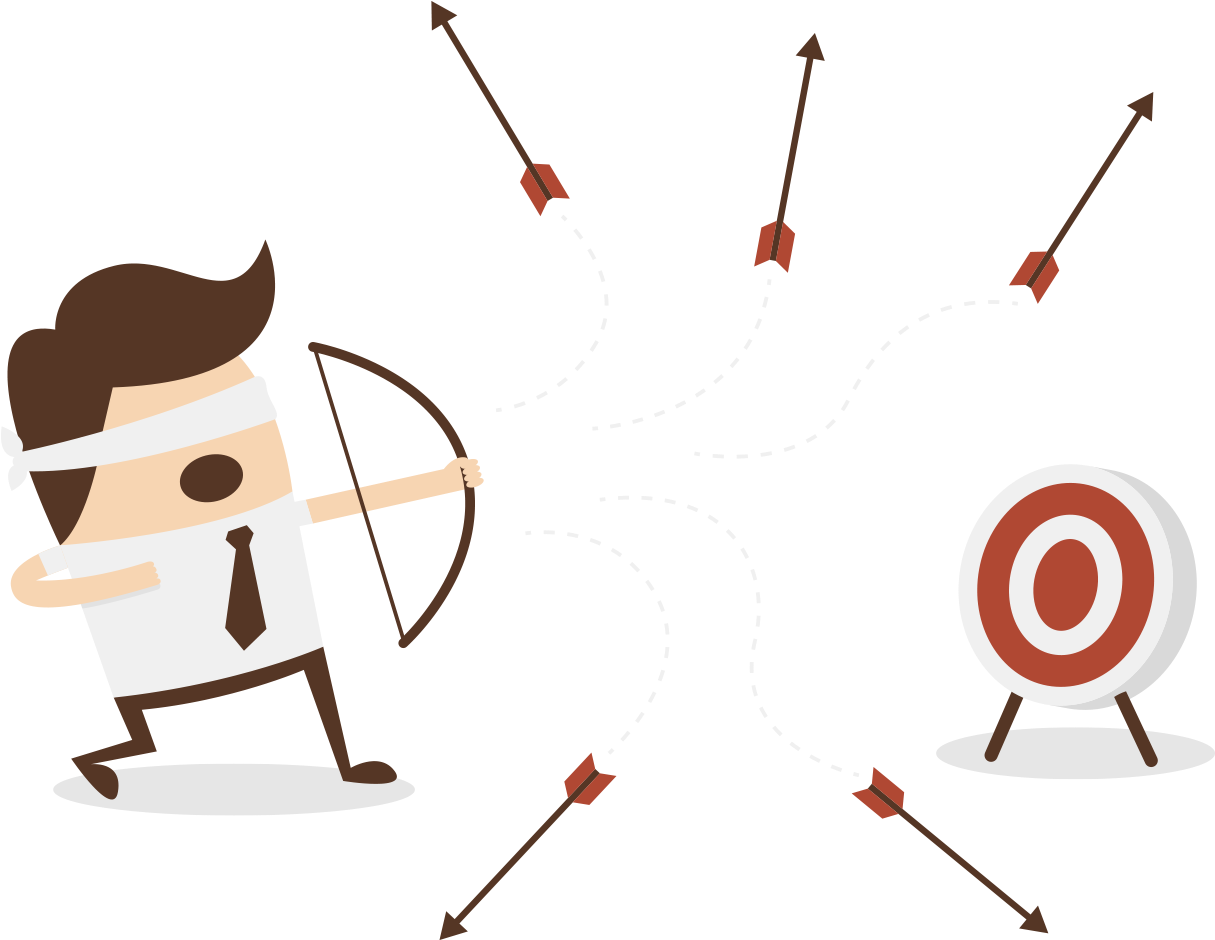
\includegraphics[width=1\textwidth,height=\textheight]{./pictures/clipart2906322_personal_use_only.png}}

}

\end{figure}

\bookmarksetup{startatroot}

\hypertarget{sec-vorwort}{%
\chapter*{Vorwort}\label{sec-vorwort}}
\addcontentsline{toc}{chapter}{Vorwort}

\markboth{Vorwort}{Vorwort}

Dieses Buch enthält Begleittexte und Übungsvorschläge für das
Studienfach \emph{Versprecher} (sl. \emph{Jezikovni spodrsljaji}, en.
\emph{speech errors}), das im Rahmen des Germanistikstudiums an der
Universität Maribor als Wahlfach angeboten wird.

Das Buch wurde mit Hilfe der Programmierungssprache \texttt{R}
\url{https://www.r-project.org/} und der von \texttt{RStudio}
\url{https://www.rstudio.com/} entwickelten Skriptsprache
\texttt{Rmarkdown} \url{https://rmarkdown.rstudio.com/} auf der
Entwickler-Platform \texttt{Github} \url{https://github.com/} als
\texttt{Quarto\ Book} \url{https://quarto.org/} veröffentlicht.

\part{Unbewusste Fehlleistungen}

\hypertarget{sec-einfuhrung}{%
\chapter{Einführung}\label{sec-einfuhrung}}

In diesem Buch besprechen wir verschiedene Arten von sprachlichen
Fehlleistungen und varietäten- bzw. textsortenbedingten Abweichungen von
der standardsprachlichen Norm im Deutschen (teilweise auch im
Slowenischen), die im Rahmen verschiedener Forschungsbereiche (Psycho-
und Neurolinguistik, Spracherwerb, Sprachvarietäten, \ldots) diskutiert
werden und auch für germanistische Studien von Interesse sein
können.\footnote{Dieses Buch wurde mit \texttt{Quarto}
  \url{https://quarto.org/docs/books/} zusammengestellt.}

Hinweise\footnote{Clipart von \url{https://www.clipartmax.com/}}:

Das ist eine Definition (rmdnote).

Das ist ein Tip oder eine Info (rmdtip).

Das ist ein Arbeitsvorschlag (rmdrobot).

Das ist der RStudio Logotyp (rmdrstudio).

Das ist eine Warnung (rmdwarning).

Das ist eine Fehlermeldung (rmderror).

\hypertarget{sec-gegenstand}{%
\chapter{Gegenstand}\label{sec-gegenstand}}

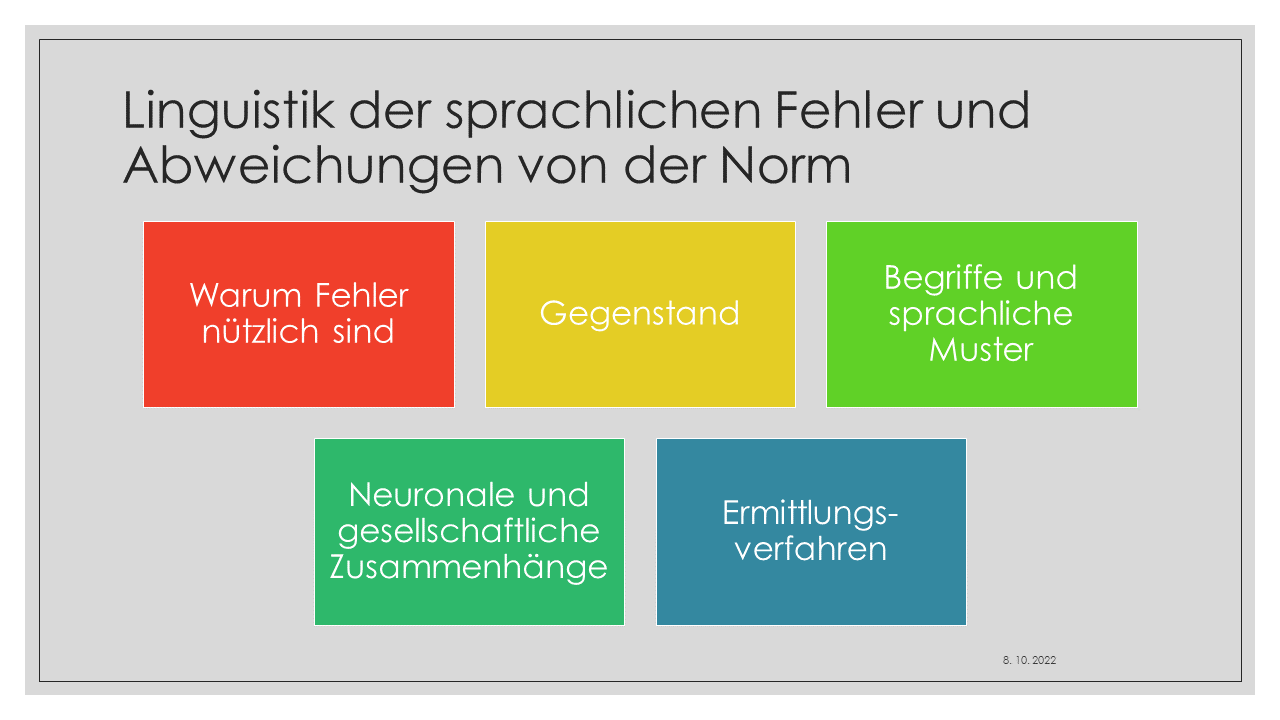
\includegraphics[width=1\textwidth,height=\textheight]{./pictures/Diapozitiv5.PNG}

In diesem Buch besprechen wir verschiedene Arten von sprachlichen
Fehlleistungen und varietäten- bzw. textsortenbedingten Abweichungen von
der standardsprachlichen Norm im Deutschen (teilweise auch im
Slowenischen), die im Rahmen verschiedener Forschungsbereiche (Psycho-
und Neurolinguistik, Spracherwerb, Sprachvarietäten, \ldots) diskutiert
werden und auch für germanistische Studien von Interesse sein können.
Berücksichtigt werden folgende sprachliche Erscheinungen:\\

\begin{itemize}
\tightlist
\item
  Zungenbrecher (en. tongue twisters, sl. lomilci jezika),\\
\item
  Zungenspitzen-Phänomen (en. tip of the tongue phenomenon, sl. izraz na
  konici jezika),\\
\item
  Versprecher (en. speech errors, spoonerisms, sl. jezikovni
  spodrsljaji),\\
\item
  sprachliche Fehler und Abweichungen im Spracherwerb (in diesem Buch
  mit Beschränkung auf den Erwerb der Zweit- und Fremdsprache),\\
\item
  Abweichungen von der standardsprachlichen Norm in neueren
  Kommunikationsformen (z.B. Chats, Sms, u.ä.),\\
\item
  Abweichungen von der standardsprachlichen Norm in multikulturellen
  Gemeinschaften (z.B. Kiezdeutsch),\\
\item
  und sprachliche Probleme und Fehlleistungen bei der Anwendung von
  gendergerechter Sprache (Ersatz des generischen Maskulinums durch
  potentielle Konkurrenzformen).\\
\end{itemize}

In diesem Einführungskurs machen wir Sie mit einigen der grundlegenden
Methoden zur Erfassung der linguistischen Merkmale in deutschen (und in
einigen Abschnitten auch mit slowenischen) Texten bekannt, in denen
diese sprachlichen Besonderheiten zu beobachten sind.

\hypertarget{sec-zungenbrecher}{%
\chapter{Zungenbrecher}\label{sec-zungenbrecher}}

\begin{figure}

{\centering 

\href{https://www.kissclipart.com/tongue-twister-cartoon-comics-stop-consonant-m2n92r/}{
\includegraphics[width=1\textwidth,height=\textheight]{./pictures/kissclipart-tongue-twister-cartoon-comics-stop-consonant-82fba1d0b8543744.png}}

}

\end{figure}

\hypertarget{was-sind-zungenbrecher}{%
\section{Was sind Zungenbrecher?}\label{was-sind-zungenbrecher}}

\emph{Zungenbrecher} (en. tongue twisters, sl. lomilci jezika), auch
zuweilen \emph{Lautüberfüllungen} genannt, sind ein bekanntes Phänomen
sowohl beim Erwerb einer Sprache als auch in der alltäglichen
Kommunikation, etwa in den öffentlichen Medien. Zungenbrecher sind
beliebt, werden von zahlreichen Sprachteilnehmern gesammelt und dienen
einerseits zur Belustigung oder Belebung eines Gesprächs oder des
Unterrichts, andererseits aber auch zu Schulungszwecken, da sie auch
beim Sprachtraining professioneller Mediensprecher von Nutzen sein
können.\footnote{https://de.wikipedia.org/wiki/Zungenbrecher}

17 Zungenbrecher innerhalb einer Minute von
\href{https://www.youtube.com/watch?v=VORRlhE7Hgk}{Rap Squad One}:

\url{https://www.youtube.com/embed/VORRlhE7Hgk}

Bei Zungenbrechern handelt es sich um Lautfolgen, deren Aussprache nicht
nur Lernern einer fremden Sprache schwerfällt sondern auch
Erstsprachlern, insbesondere bei höherer Sprechgeschwindigkeit und auch
bei Wiederholungsversuchen zu Korrekturzwecken. Die Aussprache von
vielen Lautfolgen ist in der Erstsprache hochautomatisiert, so dass
gängige Lautkombinationen in sprachlichen Äußerungen gewöhnlich kein
Ausspracheproblem darstellen. Die Fehlerrate ist in der alltäglichen
sprachlichen Kommunikation gering. In sprachlichen Konstruktionen, die
sich als Zungenbrecher herausstellen, kommen jedoch ungewohnte
Wortabfolgen, ähnliche Laute und Silben oder Wörter, die sich
geringfügig voneinander unterscheiden, gehäuft vor. Diese Abweichungen
von gewohnten sprachlichen Konstruktionen erfordert erhöhte
Konzentration.

\hypertarget{zungenbrecher-typen}{%
\section{Zungenbrecher-Typen}\label{zungenbrecher-typen}}

Einige Zungenbrecher beruhen auf dem \emph{schnellen Wechsel}\\
- zwischen \emph{ähnlichen}, aber unterschiedlichen \emph{Phonemen}
(z.B. \textless s\textgreater{} {[}s{]} und \textless sch\textgreater{}
{[}ʃ{]} ),\\
- der Kombination von zwei verschiedenen Alternationsmustern,\\
- vertrauten Konstruktionen in Lehnwörtern\\
- oder anderen Merkmalen einer gesprochenen Sprache,\\
um schwer artikulierbar zu sein.

Zum Beispiel wurde der folgende Satz von William Poundstone als ``der
schwierigste der üblichen englischsprachigen Zungenbrecher''
bezeichnet.\footnote{https://en.wikipedia.org/wiki/Tongue\_twister}

\begin{tcolorbox}[enhanced jigsaw, rightrule=.15mm, arc=.35mm, breakable, colframe=quarto-callout-note-color-frame, left=2mm, colback=white, bottomrule=.15mm, toprule=.15mm, leftrule=.75mm, opacityback=0]
\begin{minipage}[t]{5.5mm}
\textcolor{quarto-callout-note-color}{\faInfo}
\end{minipage}%
\begin{minipage}[t]{\textwidth - 5.5mm}

\textbf{Beispiel}\vspace{2mm}

\emph{The seething sea ceaseth and thus the seething sea sufficeth
us.}\\
(Das brodelnde Meer hört auf zu brodeln, und so genügt uns das brodelnde
Meer.)

\end{minipage}%
\end{tcolorbox}

Diese absichtlich schwierigen Ausdrücke waren im 19. Jahrhundert sehr
beliebt. Der beliebte Zungenbrecher ``she sells seashells'' wurde
ursprünglich 1850 als Sprachübung veröffentlicht. Der Begriff
\emph{tongue twister} (Zungenbrecher) wurde erstmals 1895 für diese Art
von sprachlichen Ausdrücken verwendet.

Eine Reihe von Zungenbrechern verwendet eine Kombination aus
\emph{Alliteration} und \emph{Reim}. Sie bestehen aus zwei oder mehr
Lautfolgen, bei denen die Zunge zwischen den Silben neu positioniert
werden muss, dann werden dieselben Laute in einer anderen Reihenfolge
wiederholt.

\begin{tcolorbox}[enhanced jigsaw, rightrule=.15mm, arc=.35mm, breakable, colframe=quarto-callout-note-color-frame, left=2mm, colback=white, bottomrule=.15mm, toprule=.15mm, leftrule=.75mm, opacityback=0]
\begin{minipage}[t]{5.5mm}
\textcolor{quarto-callout-note-color}{\faInfo}
\end{minipage}%
\begin{minipage}[t]{\textwidth - 5.5mm}

\textbf{Beispiel}\vspace{2mm}

\emph{Fischers Fritze fischt frische Fische, frische Fische fischt
Fischers Fritze}

\end{minipage}%
\end{tcolorbox}

In anderen Zungenbrechern werden zusammengesetzte Wörter
(\emph{Komposita}) und ihre \emph{Stämme} genutzt, um die Artikulation
zu erschweren.

\begin{tcolorbox}[enhanced jigsaw, rightrule=.15mm, arc=.35mm, breakable, colframe=quarto-callout-note-color-frame, left=2mm, colback=white, bottomrule=.15mm, toprule=.15mm, leftrule=.75mm, opacityback=0]
\begin{minipage}[t]{5.5mm}
\textcolor{quarto-callout-note-color}{\faInfo}
\end{minipage}%
\begin{minipage}[t]{\textwidth - 5.5mm}

\textbf{Beispiel}\vspace{2mm}

\href{https://en.wikipedia.org/wiki/How_much_wood_would_a_woodchuck_chuck}{Woodchuck}\\
How much wood would a woodchuck chuck\\
if a woodchuck could chuck wood?\\
A woodchuck would chuck all the wood he could chuck\\
if a woodchuck would chuck wood.\\

\end{minipage}%
\end{tcolorbox}

Andere Zungenbrecher haben die Form eines Wortes oder \emph{kurzen
Phrase}, die sich bei schneller Wiederholung als Zungenbrecher
entpuppen.

\begin{tcolorbox}[enhanced jigsaw, rightrule=.15mm, arc=.35mm, breakable, colframe=quarto-callout-note-color-frame, left=2mm, colback=white, bottomrule=.15mm, toprule=.15mm, leftrule=.75mm, opacityback=0]
\begin{minipage}[t]{5.5mm}
\textcolor{quarto-callout-note-color}{\faInfo}
\end{minipage}%
\begin{minipage}[t]{\textwidth - 5.5mm}

\textbf{Beispiele}\vspace{2mm}

Neu-Schwanstein\\

Toy boat\\
Cricket critic\\
Unique New York\\
A proper copper coffee pot\\
Red leather, yellow leather\\
Irish wristwatch, Swiss wristwatch\\
Peggy Babcock\\

\end{minipage}%
\end{tcolorbox}

In manchen Fällen ergibt die inkorrekte Wiedergabe eines Spruchs einen
vulgären sprachlichen Ausdruck, was wiederum der Belustigung dient.

\begin{tcolorbox}[enhanced jigsaw, rightrule=.15mm, arc=.35mm, breakable, colframe=quarto-callout-note-color-frame, left=2mm, colback=white, bottomrule=.15mm, toprule=.15mm, leftrule=.75mm, opacityback=0]
\begin{minipage}[t]{5.5mm}
\textcolor{quarto-callout-note-color}{\faInfo}
\end{minipage}%
\begin{minipage}[t]{\textwidth - 5.5mm}

\textbf{Beispiele}\vspace{2mm}

\emph{Kaplan zdaj spi, zdaj je.}\\

Old Mother Hunt had a rough cut punt\\
Not a punt cut rough,\\
But a rough cut punt.\\

\end{minipage}%
\end{tcolorbox}

Einige Zungenbrecher wirken selbst bei korrekter Aussprache lustig:\\

\begin{tcolorbox}[enhanced jigsaw, rightrule=.15mm, arc=.35mm, breakable, colframe=quarto-callout-note-color-frame, left=2mm, colback=white, bottomrule=.15mm, toprule=.15mm, leftrule=.75mm, opacityback=0]
\begin{minipage}[t]{5.5mm}
\textcolor{quarto-callout-note-color}{\faInfo}
\end{minipage}%
\begin{minipage}[t]{\textwidth - 5.5mm}

\textbf{Beispiele}\vspace{2mm}

Are you copperbottoming those pans, my man?\\
No, I'm aluminiuming 'em Ma'am.\\
Pad kid poured curd pulled cold

\end{minipage}%
\end{tcolorbox}

\hypertarget{verwechselbare-phoneme}{%
\section{Verwechselbare Phoneme}\label{verwechselbare-phoneme}}

Die klangliche Ähnlichkeit und Artikulationsähnlichkeit von bestimmten
Sprachlauten scheint die Häufigkeit von sprachlichen Fehlleistungen zu
fördern.

Im Englischen werden die folgenden Phoneme häufig verwechselt:\\
- /l/ mit /r/ (z.B. \emph{lot}, \emph{rot}),\\
- /s/ mit /ʃ/ (z.B. \emph{sip}, \emph{ship}).\\
- /f/ mit /p/ (z.B. \emph{fit}, \emph{pit}),\\
- /w/ mit /r/ (z.B. \emph{which}, \emph{rich})\\
- u.a. laut einer MIT
Konfusionsmatrix\footnote{Wikipedia}(https://en.wikipedia.org/wiki/Tongue\_twister)

Bestimmte Phoneme sind \emph{schwieriger auszusprechen} als andere. Im
Englischen kann man davon ausgehen, dass {[}tʃ{]} wie im Anlaut von en.
\textless chair\textgreater{} schwieriger ist als ch {[}tʃ{]} wie in
\textless share\textgreater, was bei entsprechender Verteilung im Satz
einen Zungenbrecher heraufbeschwören
kann.\footnote{Wikipedia}(https://en.wikipedia.org/wiki/Tongue\_twister)
Dies führt gewöhnlich dazu, dass der schwierigere Laut durch den
einfacheren \emph{ersetzt} wird oder sogar \emph{getilgt} wird.
Entsprechendes gilt auch für Lenes (schwache Konsonanten) im Vergleich
zu Fortes (starken Konsonanten). \emph{Starke Konsonanten} (z.B. /ptk/
im Vergleich zu /bdg/) kommen in der Sprache häufiger vor, entwickeln
sich im Spracherwerb früher und bekommen in phonologischen
Phonemhierarchien Basispositionen zugewiesen. In Zungenbrechern werden
schwierigere Sprachlaute daher häufiger mit starken Konsonanten ersetzt.

Zungenbrecher sind sprachspezifisch. In bestimmten Sprachen können
beispielsweise auch die unterschiedliche Dauer von Vokalen oder
prosodische Unterschiede zwischen Silben eine Rolle bei der Entstehung
von Zungenbrechern spielen (etwa die Vokallänge).

--\textgreater{}
\href{https://en.wikipedia.org/wiki/Malapropism}{Malapropismus}: Texas
has a lot of electrical votes (electoral).\\
--\textgreater{}
\href{https://en.wikipedia.org/wiki/Spoonerism}{Spoonerismus}:
verwechselte Sprachlaute in Wörtern und Phrasen.\\
--\textgreater{}
\href{https://en.wikipedia.org/wiki/Shibboleth}{Shibboleth}: Wort oder
Phrase, die die Gruppenzugehörigkeit einer Person oder die Ausgrenzung
von sozialen Gruppen ermöglicht (z.B. aufgrund der Aussprache, die nur
von Einheimischen entsprechend realisiert wird und nicht von
Außenseitern oder Fremden).\\

In \emph{Hip-Hop oder Rap-Musiktexten} sind Zungenbrecher nicht selten.

Sprachliche Fehlleistungen wie die Zungenbrecher sind nicht nur auf die
Lautsprache beschränkt, sondern auch in der Gebärdensprache beobachtbar
(z.B. \emph{Vergebärdler}).

\hypertarget{erkluxe4rungsversuche}{%
\section{Erklärungsversuche}\label{erkluxe4rungsversuche}}

Was ist die \emph{Ursache} für aussprachebedingte sprachliche
Fehlleistungen?

Außer artikulatorischer und klanglicher Ähnlichkeit scheint die
Ähnlichkeit der Muskelbewegungen und ihre Repräsentation im Gehirn eine
Rolle bei der Entstheung von sprachlichen Fehlleistungen wie den
Zungenbrechern zu spielen.

Erkärungsversuch, veröffentlicht in der wissenschaftlichen Zeitschrift
\href{https://www.nature.com/articles/nature.2013.12471.pdf}{Nature}:\\

Ausgefeilte mehrdimensionale statistische Verfahren ermöglichten es den
Forschern, die riesigen Datenmengen zu sichten und aufzudecken wie
grundlegende neuronale Bausteine -- Muster von Neuronen, die im Laufe
der Zeit an verschiedenen Orten feuern -- sich kombinieren, um die
Sprachlaute des Amerikanischen Englischs zu bilden.

Die Muster für \emph{Konsonanten} waren ganz \emph{anders} als für
\emph{Vokale}, auch wenn die Sprechlaute genau die \emph{gleichen Teile
des Vokaltrakts nutzen}, sagt der Autor Edward Chang, ein
Neurowissenschaftler an der University of California in San Francisco.

\emph{Die Lippen, die Zähne, die Zungenspitze}

Die verschiedenen Muster könnten helfen zu erklären, warum
\emph{Versprecher} auf vorhersehbare Weise auftreten: Wir vertauschen
oft zwei Konsonanten in sogenannte \emph{Spoonerismen} (en. `Boat-Tag'
statt en. `Tote Bag') oder verwechseln zwei Vokale (`wheel' (Rad) für
`whale' Wal), tauschen aber \emph{selten Konsonanten gegen Vokale} aus.4

Das Team fand auch heraus, dass das Gehirn die Artikulation anscheinend
nicht nach dem \emph{Klang} der resultierenden Phoneme koordiniert, wie
bisher vermutet, sondern wie sich die \emph{Muskeln bewegen} müssen.

\begin{tcolorbox}[enhanced jigsaw, titlerule=0mm, arc=.35mm, breakable, opacitybacktitle=0.6, title=\textcolor{quarto-callout-important-color}{\faExclamation}\hspace{0.5em}{Phonemkategorien (nach Muskelbewegungen)}, colframe=quarto-callout-important-color-frame, leftrule=.75mm, rightrule=.15mm, coltitle=black, colbacktitle=quarto-callout-important-color!10!white, bottomtitle=1mm, left=2mm, colback=white, toptitle=1mm, bottomrule=.15mm, toprule=.15mm, opacityback=0]

Die Daten ergaben \emph{drei Kategorien von Konsonanten}:\\
- koronale Konsonanten, ausgesprochen mit dem vorderen Zungenrand (wie
/z/ im Anlaut des Wortes \textless Seife\textgreater{} ),\\
- velare Konsonanten, ausgesprochen mit dem hinteren Zungenblatt (wie
/g/ im Anlaut des Wortes \textless Gas\textgreater{} ) und\\
- labiale Konstonanten, ausgesprochen mit den Lippen (wie /m/ im Anlaut
des Wortes \textless Mus\textgreater{} ).

\emph{Vokale} teilen sich in \emph{zwei Gruppen} auf:\\
- gerundete Vokale (wie /u/ in \textless Lu-pe\textgreater{} ) und\\
- ungerundete Vokale (wie /a/ in \textless La-de\textgreater{} ).

\end{tcolorbox}

Das impliziert, dass \emph{Zungenbrecher} harte Aussprachebrocken sind,
weil sich (laut Chang) ``die \emph{Repräsentationen} im Gehirn stark
\emph{überlappen}''.

\begin{tcolorbox}[enhanced jigsaw, rightrule=.15mm, arc=.35mm, breakable, colframe=quarto-callout-note-color-frame, left=2mm, colback=white, bottomrule=.15mm, toprule=.15mm, leftrule=.75mm, opacityback=0]
\begin{minipage}[t]{5.5mm}
\textcolor{quarto-callout-note-color}{\faInfo}
\end{minipage}%
\begin{minipage}[t]{\textwidth - 5.5mm}

\textbf{Beispiel}\vspace{2mm}

Zum Beispiel werden `/s/' und `/š/' beide im Gehirn als
Front-of-the-Tongue-Sounds (\emph{koronale} Laute) gespeichert, so dass
das Gehirn diese wahrscheinlich \emph{häufiger verwechselt} als Laute,
die von \emph{verschiedenen Teilen} der Zunge bzw. Sprechwerkzeuge
gebildet werden (z.B. /s/ vs.~/m/).

\end{minipage}%
\end{tcolorbox}

\begin{tcolorbox}[enhanced jigsaw, rightrule=.15mm, arc=.35mm, breakable, colframe=quarto-callout-note-color-frame, left=2mm, colback=white, bottomrule=.15mm, toprule=.15mm, leftrule=.75mm, opacityback=0]
\begin{minipage}[t]{5.5mm}
\textcolor{quarto-callout-note-color}{\faInfo}
\end{minipage}%
\begin{minipage}[t]{\textwidth - 5.5mm}

\textbf{Beispiel}\vspace{2mm}

\emph{Sally sells seashells} (Sally verkauft Muscheln) ist knifflig.\\
\emph{Mally sells sea-smells} (Mally verkauft Meeresgerüche) ist es
nicht.

\end{minipage}%
\end{tcolorbox}

\begin{enumerate}
\def\labelenumi{\arabic{enumi}.}
\tightlist
\item
  Öffnen Sie die Video-Datei auf YouTube
  (https://www.youtube.com/watch?v=wuK\_znJRKhU) mit 11 schwierigen
  Sprüchen auf Ihrem Computer -- und stoppen Sie die Wiedergabe.\\
\item
  Öffnen Sie ein Programm zur Aufnahme Ihrer Stimme (Praat, Windows
  Recorder, Audacity, Sony Soloist \ldots), setzen Sie Ihr Headset
  (Kopfhörer mit Mikrofon) auf und drücken Sie Aufnahme.\\
\item
  Spielen Sie die bereits geöffnete Video-Datei mit den elf deutschen
  Zungenbrechern ab.\\
\item
  Lesen Sie die Zungenbrecher nacheinander vom Bildschirm ab, sprechen
  sie diesen möglichst schnell und ohne Fehler ins Mikrofon. Die Zeit
  für jeden Zungenbrecher ist beschränkt. Jeder der elf Zungenbrecher
  soll von Ihnen vollständig ausgesprochen werden. Gewöhnlich werten wir
  den ersten Durchgang für die folgende Analyse. Wiederholen Sie
  eventuell nur diejenigen Zungenbrecher, die Sie nicht zu Ende
  ausgesprochen haben (z.B. wegen Zeitmangel oder weil Sie verwirrt
  waren).\\
\item
  Laden Sie Ihre Aufnahme als erste Aufgabe (assignment) hoch (Aufgabe
  N01).\\
\end{enumerate}

Nach dem Lesen aller elf Sprüche hören Sie sich Ihre Aufnahme mit allen
Zungenbrechern an und stellen Sie fest, welche Fehler Sie gemacht haben!

Tragen Sie die Zungenbrecher und Ihre Klassifizierung der Fehler in die
\emph{gemeinsame Zungenbrecher-Tabelle} nach dem dort vrogegebenen
Schema ein!

\hypertarget{sec-zungenspitze}{%
\chapter{Zungenspitzen-Phänomen}\label{sec-zungenspitze}}

\begin{figure}

{\centering 

\href{https://web.colby.edu/cogblog/tag/tip-of-the-tongue/}{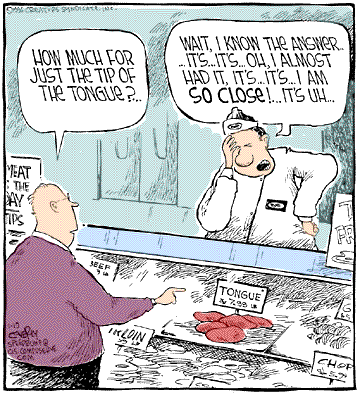
\includegraphics[width=1\textwidth,height=\textheight]{./pictures/tip-of-the-tongue1-1.png}}

}

\end{figure}

Das \emph{Zungenspitzenphänomen}\footnote{\href{https://de.wikipedia.org/wiki/Zungenspitzenph\%C3\%A4nomen}{Wikipedia}}
(TOT-Phänomen, von en. \emph{tip-of-the-tongue}) bezeichnet einen
Zustand, in dem ein eigentlich bekanntes Wort zu einem bestimmten
Zeitpunkt im mentalen Lexikon nicht oder nur teilweise verfügbar
ist.\footnote{Brown, Roger / McNeill, David (1966): The „tip of the
  tongue`` phenomenon. In: Journal of Verbal Learning and Verbal
  Behaviour 5, 325.}

Wenn eine Person ein Wort nicht wiedergeben kann, obwohl sie davon
überzeugt ist, es eigentlich zu kennen, tritt das \textbf{TOT-Phänomen}
und somit die Wortfindungssuche ein. Häufig wird der Zustand begleitet
von dem frustrierenden Gefühl, dass sich der Ausdruck in mental
„greifbarer`` Nähe befindet, sozusagen „auf der Zunge
liegt``.\footnote{Schwartz, Bennett L. (1999): Sparkling at the end of
  the tongue: The etiology of tip-of-the-tongue phenomenology. In:
  Psychonomic Bulletin \& Review 6 (3), 381.}

\begin{tcolorbox}[enhanced jigsaw, rightrule=.15mm, arc=.35mm, breakable, colframe=quarto-callout-note-color-frame, left=2mm, colback=white, bottomrule=.15mm, toprule=.15mm, leftrule=.75mm, opacityback=0]
\begin{minipage}[t]{5.5mm}
\textcolor{quarto-callout-note-color}{\faInfo}
\end{minipage}%
\begin{minipage}[t]{\textwidth - 5.5mm}

\textbf{Beispiel}\vspace{2mm}

Herr P. kann den Namen eines slowenischen Ensembles (\emph{Modrijani},
z.B. \href{https://www.youtube.com/watch?v=a7pcqxKHb_E}{Tebi} oder
\href{https://www.youtube.com/watch?v=RuiBoAWfSJE}{Ti, moja rožica}) oft
nicht abrufen. Er weiß, dass der Name der Band mit dem Laut \emph{M}
beginnt und drei oder vier Silben hat. Aber der Name einer britischen
Band (\emph{The Monkeys}, z.B.
\href{https://www.google.com/search?client=firefox-b-d\&q=the+monkeys\#fpstate=ive\&vld=cid:38a2b68e,vid:wB9YIsKIEbA,st:0}{I'm
a Believer}), die in den 1960er Jahren bekannt war und die Herr P. in
seiner Jugend kennenlernte, scheint den Abruf des richtigen Namens aus
dem Langzeitgedächtnis zu blockieren, denn auch dieser Bandname beginnt
mit einem \emph{M}.

\end{minipage}%
\end{tcolorbox}

\begin{figure}

{\centering 

\href{https://www.deviantart.com/iamarg/art/The-Tip-of-the-Tongue-414103082}{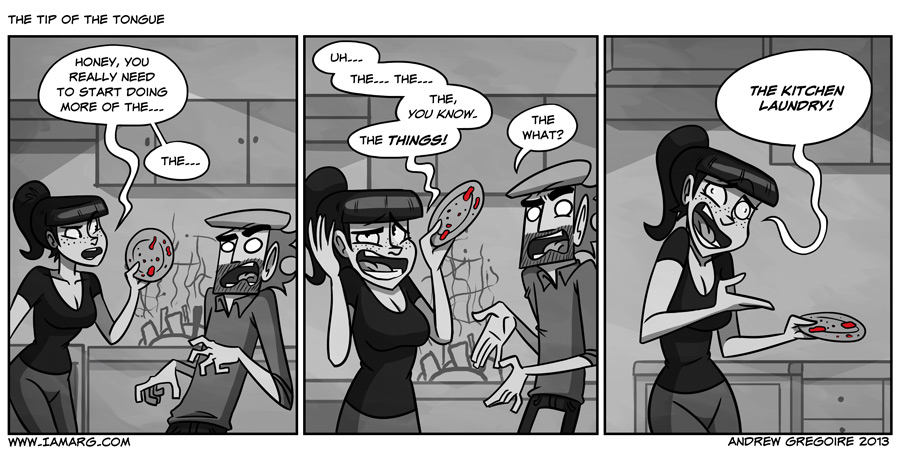
\includegraphics[width=1\textwidth,height=\textheight]{./pictures/d6ujnze-d76188d2-5723-46fc-933e-afe0459b1d08.jpg}}

}

\end{figure}

\hypertarget{warum-sind-tots-interessant}{%
\section{Warum sind TOTs
interessant?}\label{warum-sind-tots-interessant}}

\href{https://memucho.de/Tip-of-the-Tongue-Phaenomen/983\#}{Memucho}:

\begin{itemize}
\item
  Bei TOTs handelt es sich um ein \emph{universelles Phänomen}, das laut
  Umfrage von Schwartz (1999)\footnote{Schwartz, B. L., \& Metcalfe, J.
    (2011). Tip-of-the-tongue (TOT) states: retrieval, behavior, and
    experience. Memory \& Cognition, 39(5), 737--749.} in vielen
  Sprachen mit einer ähnlichen Metapher beschrieben wird und sowohl bei
  Kindern als auch Erwachsenen auftritt.
\item
  TOTs sind \emph{alltagsrelevant}. Je nach Lebenssituation (Alter,
  häufige Abfrage-Kontexte) tritt ein TOT-Zustand durchschnittlich ein
  Mal pro Woche bis ein Mal am Tag auf.
\item
  Ein TOT-Zustand wird als \emph{emotional} quälendes \emph{bewusstes}
  Erlebnis wahrgenommen. Daher strebt der Betroffene nach Auflösung des
  Zustands.
\item
  TOTs lassen sich gut generieren und damit \emph{experimentell
  untersuchen}.
\end{itemize}

\href{https://www.daserste.de/information/wissen-kultur/w-wie-wissen/videos/Gedaechtnisstreiche-video-100.html}{ARD
Mediathek}

\url{https://pdvideosdaserste-a.akamaihd.net/int/2019/12/07/54a08c0c-a5c9-447d-b816-12e097411422/960-1_569889.mp4}

\hypertarget{erkluxe4rungsansuxe4tze}{%
\section{Erklärungsansätze}\label{erkluxe4rungsansuxe4tze}}

\href{https://memucho.de/Tip-of-the-Tongue-Phaenomen/983\#}{Memucho}:

Bei der Unterschung von TOTs lassen sich zwei Betrachtungsebenen
unterscheiden.

\hypertarget{die-direct-access-sichtweise}{%
\subsection{Die
direct-access-Sichtweise}\label{die-direct-access-sichtweise}}

Bei dieser Sichtweise fokussiert man sich auf den Gedächtnisprozess an
sich. Ein TOT-Zustand wird als Zeichen für einen verhinderten Abruf
betrachtet. Dazu existieren zahlreiche Erklärungsansätze. In einem
aktuellen \emph{Modell von Gollan und Brown (2006)} nimmt man an, dass
der TOT-Zustand das Ergebnis eines \emph{unvollständigen Abrufs} ist. So
können Wortbedeutung und vereinzelte semantische Informationen abgerufen
werden, es fehlen jedoch Informationen, die eine Zusammensetzung zum
Zielwort ermöglichen würden. Die \emph{phonetische} Information kann
\emph{nicht abgerufen} werden, so dass die Sprachausgabe blockiert ist.

\hypertarget{die-metakognitive-betrachtungsebene}{%
\subsection[Die Metakognitive Betrachtungsebene]{\texorpdfstring{Die
Metakognitive
Betrachtungsebene\footnote{Metakognitionen: Gedanken über das eigene
  Denken}}{Die Metakognitive Betrachtungsebene}}\label{die-metakognitive-betrachtungsebene}}

Hier liegt der Fokus vor allem auf der Funktion eines TOT-Erlebnisses im
Alltag. Ein TOT-Zustand wird nicht als ``\emph{Fehlermeldung}''
interpretiert, sondern als Signal dafür, dass eine gewisse Menge an
\emph{Informationen über ein Zielwort verfügbar} ist, die einen
erfolgreiche \emph{Abruf unter weiterer Anstrengung möglich} macht.
Damit geht mit einem TOT-Erlebnis ein \emph{motivationaler} Prozess
einher.

Beim Lernen kommt das eben erwähnte Motivationspotential ins Spiel.
Aktuelle Forschung schlägt die folgende Interpretation vor: Ein
TOT-Zustand könnte als eine Art ``\emph{Marker}'' funktionieren, der
\emph{optimal erlernbare}, jedoch noch \emph{nicht vollständig
gefestigte Gedächtnisinhalte} kennzeichnet. Die Hypothese steht in
Einklang mit Erkenntnissen aus der Lerntheorie, die besagen, dass
\emph{Informationen am leichtesten gelernt} werden, die \emph{weder
mühelos abrufbar noch vollkommen neu} sind. Diese Markerfunktion könnte
evolutionär adaptiv sein und so den ``\emph{Sinn}'' eines TOT-Zustandes
erklären. Eindeutige empirische Belege gibt es hierzu allerdings nicht.

\hypertarget{methodologie}{%
\section{Methodologie}\label{methodologie}}

\href{https://memucho.de/Tip-of-the-Tongue-Phaenomen/983\#}{Memucho}:

Allgemein kann einen TOT-Zustand sowohl naturalistisch (rückblickend
oder in Form von Tagebucheinträgen) als auch experimentell erforscht
werden. In beiden Fällen sind einige Punkte zu beachten.

\begin{itemize}
\item
  Es hat sich als wichtig herausgestellt, einen TOT-Zustand genau zu
  \emph{definieren und abzugrenzen} gegenüber dem Nicht-Wissen, dem
  definitiven Wissen und einem sogenannten ``Feeling-of-knowing'',
  charakterisiert dadurch, dass eine Person erwartet, das Zielwort
  wiederzuerkennen (\emph{recognition}), es aber nicht selber
  produzieren kann (\emph{kein recall}).
\item
  Erhoben wird im Falle eines TOTs in der Regel, welche semantischen
  \emph{Einzelinformationen zugänglich} sind (Anfangsbuchstabe,
  Wortlänge, Wortbedeutung,\ldots) und ob der TOT-Zustand am Ende
  aufgelöst werden konnte oder nicht.
\end{itemize}

Beim experimentellen Vorgehen werden TOTs in den meisten Fällen
hervorgerufen, indem den Studienteilnehmenden \emph{komplizierte
Definitionen} vorgelegt und das definierte Wort erfragt wird. Auf diese
Art und Weise lassen sich TOTs zuverlässig generieren. Alternativ wurden
z.B. \emph{Bilder} von berühmten Personen gezeigt und deren Name
erfragt. In den unten angeführten Untersuchungen werden noch einige
andere Methoden beschrieben.

\hypertarget{vorkommen-und-huxe4ufigkeit-des-tot-phuxe4nomens}{%
\section{Vorkommen und Häufigkeit des
TOT-Phänomens}\label{vorkommen-und-huxe4ufigkeit-des-tot-phuxe4nomens}}

Das Zungenspitzenphänomen wird, ähnlich wie Versprecher, nicht auf
organische oder gesundheitliche Ursachen zurückgeführt. Die meisten
Menschen erleben mindestens ein TOT pro Woche, es handelt sich daher
nicht um eine außergewöhnliche, sondern vielmehr um eine
\emph{alltägliche Erscheinung}. Im Normalfall tritt die Erinnerung an
das gesuchte Wort nach kürzeren oder längeren Zeiträumen wieder ein oder
das Auffinden wird durch \emph{Stichwörter und Kontext begünstigt}.

TOTs lassen sich auch leicht \emph{experimentell hervorrufen} und eignen
sich daher gut für wissenschaftliche Studien. Forscher der
Psycholinguistik nutzen das Phänomen zur Untersuchung der Struktur des
\emph{mentalen Lexikons} und der damit verbundenen Erforschung der
\emph{Sprachproduktionsabläufe}.\footnote{Schwartz, Bennett L. (1999):
  Sparkling at the end of the tongue: The etiology of tip-of-the-tongue
  phenomenology. In: Psychonomic Bulletin \& Review 6 (3), 381.}

\hypertarget{wortfindungsprozess-im-tot-zustand}{%
\section{Wortfindungsprozess im
TOT-Zustand}\label{wortfindungsprozess-im-tot-zustand}}

Brown/McNeill untersuchten 1966 zum ersten Mal das
Zungenspitzenphänomen. Sie konfrontierten Probanden mit Definitionen
schwieriger bzw. selten gebrauchter Wörter (z. B. Nepotismus =
Vetternwirtschaft). Wenn die Testpersonen das gesuchte Zielwort nicht
sofort benennen konnten, befanden sie sich im TOT-Zustand und wurden
gebeten, einen Fragebogen auszufüllen. Die Probanden konnten Angaben
machen über:\footnote{Brown, Roger / McNeill, David (1966): The „tip of
  the tongue`` phenomenon. In: Journal of Verbal Learning and Verbal
  Behaviour 5, 325-326.}

\begin{itemize}
\tightlist
\item
  Wörter mit \emph{ähnlicher} Bedeutung oder ähnlichem Klang\\
\item
  die Anzahl der \emph{Silben}\\
\item
  die \emph{Anfangsbuchstaben}.
\end{itemize}

Brown/McNeill kamen zu dem Ergebnis, dass in ca. der \emph{Hälfte} der
Fälle die \emph{Anfangsbuchstaben} und \emph{Silbenanzahl} \emph{korrekt
benannt} werden konnten. Sowohl Wörter mit ähnlichen phonologischen als
auch mit ähnlichen semantischen Eigenschaften wurden produziert. Eine
\emph{Zweiteilung des mentalen Lexikons} in eine semantische und eine
phonologische Ebene ist daher nicht auszuschließen.{[}6{]} Studien in
anderen Sprachen konnten zeigen, dass Probanden außerdem in der Lage
waren, das \emph{Genus} (grammatische Geschlecht), die \emph{Wortart}
und den \emph{Artikel} des Zielwortes anzugeben.{[}7{]}

Anhand von Tip of the tongue(TOT)-Experimenten hat man herausgefunden,
dass Versuchspersonen, denen Definitionen von relativ ungebräuchlichen
Wörtern vorgelesen wurden (z.B. \emph{Sextant}), Wörter benennen, bei
denen 80 Prozent der genannten \emph{Anlaute} und mehr als 70 Prozent
der \emph{Auslaute} entweder dem Zielwort entsprechen oder aber ihm sehr
ähnlich sind.\footnote{https://de.wikipedia.org/wiki/Badewanneneffekt\_(Psychologie)}

Entsprechend zeigte eine andere Studie, dass man sich im Allgemeinen
\emph{leichter} an den \emph{Wortanfang} als an das Ende des Wortes
erinnert. Bei etwa 500 TOT-Situationen wurde in 51 Prozent der Fälle das
erste Phonem richtig getroffen, das letzte Phonem nur in 35
Prozent.\footnote{Giuliano Merz:
  \href{http://www.a-ch-d.eu/materialien/WOERTERimKOPF/Merz-Paget-Pet\%C3\%B6_Handout.pdf}{Das
  mentale Lexikon und die intuitive Grammatik}. Abgerufen am 8. Februar
  2019.}

\hypertarget{abhuxe4ngigkeit-von-alter-und-frequenz}{%
\section{Abhängigkeit von Alter und
Frequenz}\label{abhuxe4ngigkeit-von-alter-und-frequenz}}

Aufbauend auf den Ergebnissen von Brown/McNeill, untersuchten Burke et
al.~(1991) das Auftreten des TOT-Phänomens in Abhängigkeit von den
Faktoren \emph{Alter}, \emph{Frequenz} und \emph{zeitlicher Abstand} zur
letzten Nutzung von \emph{Eigennamen, Dingen und abstrakten Wörtern}.
Sie berufen sich in ihrer Studie auf die \emph{Node Structure Theory},
die zu den interaktiven Aktivierungsmodellen zählt. Sie besagt, dass
Informationen im mentalen Lexikon in einem \emph{Netzwerk} aus
interagierenden Knoten gespeichert sind, die wiederum aktiviert
(\emph{Priming}) werden müssen, bevor auf die Information zugegriffen
werden kann. Im TOT-Zustand sind die \emph{Verbindungen} zwischen den
Knoten \emph{geschwächt}, und ein Zugriff ist nicht möglich. So kann das
Wort z. B. auf semantischer Ebene aktiviert worden sein, die Verbindung
zur phonologischen Ebene ist aber unterbrochen, und es kann keine
Benennung des gesuchten Wortes erfolgen. Findet jedoch ein
\emph{phonologisches Priming mit Hilfe von ähnlich klingenden Wörtern}
statt, lässt sich die Anzahl der TOTs reduzieren.\footnote{Burke,
  Deborah / MacKay, Donald / Worthley, Joanna / Wade, Elizabeth (1991):
  On the Tip of the Tongue: What Causes Word Finding Failures in Young
  and Older Adults? In: Journal of Memory and Language 30, 543.}

Außerdem konnte bestätigt werden, dass \emph{ältere Personen häufiger
TOTs} erleben. Sie können sich besonders schlecht an \emph{Eigennamen}
erinnern und insgesamt \emph{weniger Teilinformationen zu den
Zielwörtern} angeben. Die Verbindungen zwischen den Knoten wird auch
geschwächt, wenn das Wort seit längerer Zeit nicht mehr abgerufen wurde
oder generell nur sehr \emph{selten gebraucht} wird.\footnote{Burke,
  Deborah / MacKay, Donald / Worthley, Joanna / Wade, Elizabeth (1991):
  On the Tip of the Tongue: What Causes Word Finding Failures in Young
  and Older Adults? In: Journal of Memory and Language 30, 542-543;555.}

\emph{Neuroimaging-Ergebnisse}: Es hat den Anschein, dass ältere und
jüngere Menschen während der TOT-Zustände ein ähnliches Netzwerk von
Hirnregionen nutzen, wie z. B. den \emph{präfrontalen Kortex}, die
\emph{linke Insula} und den \emph{sensomotorischen Kortex}. Ältere
Menschen zeigen jedoch \emph{Unterschiede in der Aktivität einiger
Bereiche} im Vergleich zu jüngeren Menschen. TOTs nehmen bei älteren
Menschen mit dem altersbedingten \emph{Verlust an grauer Substanz} in
der linken Insula zu.\footnote{Shafto, M.; Burke, D.; Stamatakis, E.;
  Tam, P.; Tyler, L. (2007). ``On the Tip-of-the-Tongue: Neural
  Correlates of increased Word-finding Failures in Normal Aging''.
  Journal of Cognitive Neuroscience. 19 (12): 2060--2070.
  doi:10.1162/jocn.2007.19.12.2060. PMC 2373253. PMID 17892392} Dies
geht mit einer geringeren Aktivität in der linken Insula einher und
steht in Zusammenhang mit einer höheren Häufigkeit von TOTs.\footnote{Shafto,
  M; Stamatatis, E.; Tam, Tyler (2009). ``Word Retrieval Failures in Old
  Age: The Relationship between Structure and Function''. Journal of
  Cognitive Neuroscience. 22 (7): 1530--1540. CiteSeerX 10.1.1.222.5809.
  doi:10.1162/jocn.2009.21321. PMID 19642890. S2CID 9197386}

Das \emph{Priming} (Bahnungseffekt)\footnote{Priming ist ein Phänomen,
  bei dem die Exposition gegenüber einem Stimulus die Reaktion auf einen
  nachfolgenden Stimulus beeinflusst, ohne dass dies bewusst gesteuert
  wird oder beabsichtigt ist. Der Priming-Effekt bezieht sich auf die
  positive oder negative Auswirkung eines schnell präsentierten Stimulus
  (Priming-Stimulus) auf die Verarbeitung eines zweiten Stimulus
  (Ziel-Stimulus), der kurz darauf erscheint. Im Allgemeinen hängt die
  Entstehung des Priming-Effekts vom Vorhandensein einer positiven oder
  negativen Beziehung zwischen Priming- und Zielreizen ab. Zum Beispiel
  wird das Wort \emph{Krankenschwester} nach dem Wort \emph{Arzt}
  schneller erkannt als nach dem Wort \emph{Brot}. - Tulving E, Schacter
  DL, Stark HA (1982). ``Priming Effects in Word Fragment Completion are
  independent of Recognition Memory''. Journal of Experimental
  Psychology: Learning, Memory, and Cognition. 8 (4): 336--342.
  doi:10.1037/0278-7393.8.4.336;
  https://en.wikipedia.org/wiki/Priming\_(psychology)} während des
Wortabrufs reduziert die Häufigkeit von TOTs und fördert den Abruf des
Zielwortes. Es hat sich gezeigt, dass ältere Erwachsene davon stärker
profitieren, was mit dem Modell der sich ausbreitenden Aktivierung
(\emph{spreading activation}) übereinstimmt, bei dem neuronale
Verbindungen bei häufiger Verwendung gestärkt werden.

\hypertarget{tots-und-priming}{%
\section{TOTs und Priming}\label{tots-und-priming}}

In der Forschung zum Priming (Bahungseffekt, Vorbahnung) und zur Übung
werden \emph{Einzelworttests} verwendet, um das Vorhandensein von
TOT-Zuständen zu beurteilen. Dabei wird der \emph{erste Buchstabe} des
Zielworts \emph{oder} ein \emph{ähnlich klingendes Wort} vorgegeben, um
die Aufmerksamkeit auf das Zielwort zu lenken. Belege für die
Nützlichkeit von Priming und Übung bei der \emph{Verringerung von
TOT-Zuständen} sind, dass die meisten Informationen in TOT-Zuständen
\emph{niedrigfrequent} sind, d.~h., dass sie seit einiger Zeit nicht
mehr verwendet oder abgerufen wurden.\footnote{Rastle, Kathleen G.;
  Burke, Deborah M. (1996). ``Priming the Tip of the Tongue: Effects of
  Prior Processing on Word Retrieval in Young and Older Adults''.
  Journal of Memory and Language. 35 (4): 586--605.
  doi:10.1006/jmla.1996.0031. S2CID 13884102} Die Häufigkeit der
Informationsverwendung kann den Abrufprozess dieser Informationen
beeinflussen.{[}Rastle, Kathleen G.; Burke, Deborah M. (1996). ``Priming
the Tip of the Tongue: Effects of Prior Processing on Word Retrieval in
Young and Older Adults''. Journal of Memory and Language. 35 (4):
586--605. doi:10.1006/jmla.1996.0031. S2CID 13884102{]} Die Präsentation
eines Primings ist nur einmal erforderlich, um die Auflösung des
TOT-Zustands zu erleichtern.\footnote{Abrams, L.; Rodriguez, E. (2005).
  ``Syntactic Class Influences Phonological Priming of Tip-of-the-Tongue
  Resolution''. Psychonomic Bulletin \& Review. 12 (6): 1018--1023.
  doi:10.3758/bf03206437. PMID 16615322} Es wurde festgestellt, dass es
wahrscheinlicher ist, dass Personen ihren TOT-Zustand \emph{überwinden},
wenn ihnen der \emph{Anfangsbuchstabe} des Wortes gegeben wird, das sie
abzurufen versuchen. Wenn das Priming-Wort eine ähnliche Phonologie wie
das Zielwort hat, wird eine \emph{Zunahme} der Häufigkeit von
\emph{TOT-Zuständen} und eine \emph{höhere Häufigkeit von richtig
erinnerten} Wörtern beobachtet, wenn der TOT-Zustand aufgelöst
wird.\footnote{Askari, N (1999). ``Priming Effects on Tip-of-the-tongue
  States in Farsi-English Bilinguals''. Journal of Psycholinguistic
  Research. 28 (2): 197--212. doi:10.1023/A:1023214509959. S2CID
  141262297} Unwillkürlich kommen \emph{falsche Wörter} in den Sinn, die
\emph{ähnliche phonologische} Merkmale wie das Zielwort
aufweisen.\footnote{Abrams, L.; Rodriguez, E. (2005). ``Syntactic Class
  Influences Phonological Priming of Tip-of-the-Tongue Resolution''.
  Psychonomic Bulletin \& Review. 12 (6): 1018--1023.
  doi:10.3758/bf03206437. PMID 16615322} \emph{Phonologische
Ähnlichkeit} kann also \emph{sowohl TOT-Zustände verringern als auch
erhöhen}. Es ist jedoch möglich, dieses Problem durch eine Änderung der
syntaktischen Klasse des Priming-Wortes zu beheben. Priming-Wörter, die
sich in der \emph{gleichen syntaktischen Klasse} wie das Zielwort
befinden, bewirken \emph{keinen Unterschied} in der
TOT-Zustandsauflösung. Die TOT-Zustandsauflösung war für Priming-Wörter
in der gleichen syntaktischen Klasse und für nicht verwandte
Priming-Wörter (non-related) gleich. Wenn das Priming-Wort in Verbindung
mit anderen, nicht verwandten Priming-Wörtern aufgelistet wird, ist die
\emph{Position} von Bedeutung: Je \emph{früher in der Liste} das
Priming-Wort steht, desto \emph{geringer} ist die
\emph{Wahrscheinlichkeit}, dass es zur Auflösung des TOT-Zustands
beiträgt.\footnote{Abrams, L.; Rodriguez, E. (2005). ``Syntactic Class
  Influences Phonological Priming of Tip-of-the-Tongue Resolution''.
  Psychonomic Bulletin \& Review. 12 (6): 1018--1023.
  doi:10.3758/bf03206437. PMID 16615322}

\hypertarget{tots-und-spracherwerb}{%
\section{TOTs und Spracherwerb}\label{tots-und-spracherwerb}}

Die Geschwindigkeit und Genauigkeit, mit der Sprecher ein Wort abrufen,
wird von dem \emph{Lebensalter} beeinflusst, in dem das Wort zum ersten
Mal gelernt wurde. Insbesondere \emph{früh erworbene Wörter} werden
tendenziell \emph{schneller und genauer benannt} als spät erworbene
Wörter (Effekt des Erwerbsalters). Es wurde beobachtet, dass die
Wahrscheinlichkeit, einen TOT-Zustand zu erleben, vom Alter abhängt, in
dem das Wort im Leben erworben wurde: \emph{mehr TOT-Zustände werden mit
spät erworbenen} als mit früh erworbenen Wörtern erreicht\footnote{Navarrete,
  E; Pastore, M; Valentini, R; Peressotti, P (2015). ``First learned
  words are not forgotten: Age-of-acquisition effects in the
  tip-of-the-tongue experience''. Memory \& Cognition. 43 (7):
  1085--1103. doi:10.3758/s13421-015-0525-3. PMID 25956729}.

In der \emph{Anzahl der TOTs}, die von Einsprachigen und Zweisprachigen
erlebt werden, wurde ein signifikanter Unterschied gefunden.\footnote{Gollan,
  T. H.; Bonanni, M. P.; Montoya, R. I. (2005). ``Proper names get stuck
  on bilingual and monolingual speakers' tip of the tongue equally
  often''. Neuropsychology. 19 (3): 278--287.
  doi:10.1037/0894-4105.19.3.278. PMID 15910114} \emph{Zweisprachige}
scheinen die gleiche Anzahl von TOTs wie Einsprachige für
\emph{Eigennamen} zu berichten, aber deutlich mehr TOTs für \emph{andere
Wörter}.\footnote{Gollan, T. H.; Bonanni, M. P.; Montoya, R. I. (2005).
  ``Proper names get stuck on bilingual and monolingual speakers' tip of
  the tongue equally often''. Neuropsychology. 19 (3): 278--287.
  doi:10.1037/0894-4105.19.3.278. PMID 15910114}

Bilinguale weisen \emph{mehr TOTs} für die \emph{weniger dominante
Sprache} auf.\footnote{Gollan, T. H.; Bonanni, M. P.; Montoya, R. I.
  (2005). ``Proper names get stuck on bilingual and monolingual
  speakers' tip of the tongue equally often''. Neuropsychology. 19 (3):
  278--287. doi:10.1037/0894-4105.19.3.278. PMID 15910114 und Gollan, T.
  H.; Silverberg, N. B. (2001). ``Tip-of-the-tongue states in
  Hebrew--English bilinguals''. Bilingualism: Language and Cognition. 4
  (1): 63--83. doi:10.1017/S136672890100013X. S2CID 145762131} Bei einer
Aufgabe zur \emph{Benennung von Bildern} waren \emph{bilinguale}
Sprecher \emph{langsamer} als Monolinguale, selbst wenn sie ihre erste
und dominante Sprache verwenden konnten. Dies könnte möglicherweise
darauf zurückzuführen sein, dass zweisprachige Sprecher die \emph{Wörter
seltener verwenden} als einsprachige.\footnote{Ivanova, I.; Costa, A.
  (2008). ``Does bilingualism hamper lexical access in speech
  production?'' (PDF). Acta Psychologica. 127 (2): 277--288.
  doi:10.1016/j.actpsy.2007.06.003. PMID 17662226} \emph{Zweisprachige}
repräsentieren auch praktisch \emph{doppelt so viele Wörter} und
\emph{zusätzliche kognitive Mechanismen} zur Aktivierung und
Inaktivierung von Sprachen. Diese Mechanismen führen zu einem
\emph{zusätzlichen Verarbeitungsaufwand}, den einsprachige Personen
nicht haben. Darüber hinaus ist das zweisprachige System auch dann, wenn
eine Aufgabe einsprachig zu sein scheint, \emph{niemals funktionell
``ausgeschaltet}''\footnote{Gollan, T. H.; Bonanni, M. P.; Montoya, R.
  I. (2005). ``Proper names get stuck on bilingual and monolingual
  speakers' tip of the tongue equally often''. Neuropsychology. 19 (3):
  278--287. doi:10.1037/0894-4105.19.3.278. PMID 15910114}.

In
\href{http://babylonia.ch/de/archiv/2008/nummer-2-08/die-kosten-der-mehrsprachigkeit-zeit-und-fehler-bei-der-wortfindung/}{Ecke(2008)}
wird die Frage diskutiert, ob sich Mehrsprachigkeit negativ auf die
Schnelligkeit und Zuverlässigkeit der lexikalischen Verarbeitung in der
Erstsprache auswirkt und ob zeitweilige Wortfindungsprobleme (TOTs) in
der Erst- und in der Zielsprache (dominant oder weniger dominant)
beobachtet werden können.

\hypertarget{tots-und-emotionen}{%
\section{TOTs und Emotionen}\label{tots-und-emotionen}}

Es ist gut dokumentiert, dass \emph{Emotionen} viele Gedächtnisvariablen
beeinflussen, z. B. die Menge der abgerufenen Erinnerungen.\footnote{Schwartz,
  BL. (Feb 2010). ``The effects of emotion on tip-of-the-tongue states''
  (PDF). Psychonomic Bulletin \& Review. 17 (1): 82--7.
  doi:10.3758/PBR.17.1.82. PMID 20081165. Retrieved 20 October 2013.} Es
ist üblich, dass Individuen TOTs Emotionen zuschreiben.\footnote{Schwartz,
  BL. (Feb 2010). ``The effects of emotion on tip-of-the-tongue states''
  (PDF). Psychonomic Bulletin \& Review. 17 (1): 82--7.
  doi:10.3758/PBR.17.1.82. PMID 20081165. Retrieved 20 October 2013.} Es
wird angenommen, dass die Mehrheit der Individuen TOTs negativ erlebt.
Emotionale TOTs werden mit größerer Wahrscheinlichkeit später abgerufen
als TOTs, mit denen keine emotionale Erfahrung verbunden war.Emotionen
und TOTs stehen in Zusammenhang mit der oben erwähnten metakognitiven
Theorie. Nach dieser Theorie informieren TOTs das kognitive System
darüber, ob die Informationen, an die man sich zu erinnern versucht,
zugänglich sind, so dass Emotionen beim Erleben von TOT eine Rolle
spielen können. Einige Untersuchungen haben gezeigt, dass Fragen, die
eine emotionale Erregung auslösen, eher zu TOTs führen als Fragen, die
keine emotionale Erregung hervorrufen. Es wurde auch festgestellt, dass
sich die emotionale Erregung auf nachfolgende Fragen oder Informationen,
die abgerufen werden, ausdehnen kann, auch wenn sie selbst keine
emotionale Erregung hervorrufen. Es wurde festgestellt, dass emotionale
Erregung die Wahrscheinlichkeit des Erlebens von TOT erhöht. Bei der
Neurobildgebung wurde auch eine Aktivierung in einigen Bereichen
festgestellt, die mit Emotionen in Verbindung gebracht werden,
insbesondere im anterioren cingulären Cortex.

\hypertarget{auswirkungen-von-gesten}{%
\section{Auswirkungen von Gesten}\label{auswirkungen-von-gesten}}

Es ist nicht bekannt, ob Gesten bei der Suche nach dem schwer fassbaren
Wort in einer TOT-Erfahrung hilfreich sind.

\hypertarget{tots-und-drogen}{%
\section{TOTs und Drogen}\label{tots-und-drogen}}

Untersuchungsergebnisse deuten darauf hin, dass \emph{Lorazepam} (eine
Droge, die zur kurzfristigen Behandlung von Angstzuständen,
Schlaflosigkeit sowie zur Sedierung aggressiver Patienten verwendet
wird) die Wahrscheinlichkeit von TOT-Zuständen nicht erhöht, aber es
\emph{hemmt} den \emph{Abruf von korrekten Antworten} und das
\emph{subjektive Gefühl} von TOT-Zuständen, was dazu führt, dass die
Teilnehmer \emph{unbewusst falsche Antworten} geben.\footnote{Bacon, E.;
  Schwartz, BL.; Paire-Ficout, L.; Izaute, M. (Jun 2007). ``Dissociation
  between the cognitive process and the phenomenological experience of
  TOT: effect of the anxiolytic drug lorazepam on TOT states''.
  Conscious Cogn. 16 (2): 360--73. doi:10.1016/j.concog.2006.05.001.
  PMID 16798012. S2CID 24903714}

\emph{Koffein}: In einem Experiment beantworteten Versuchspersonen
(Koffeingruppe vs.~Placebogruppe) 100 Fragen zum Allgemeinwissen, auf
die es jeweils eine richtige Antwort gab. Für jede Frage lasen die
Teilnehmer 10 Grundwörter, die für kurze Zeit auf einem Monitor
angezeigt wurden. Jede Liste mit 10 Priming-Wörtern enthielt zwischen
zwei und acht Wörter, die der richtigen Antwort auf die Frage
phonologisch ähnlich waren, während die übrigen Wörter keinen solchen
Bezug aufwiesen. Die Koffeingruppe hatte \emph{weniger TOT}-Erlebnisse
als die Placebogruppe, was auf ein besseres Erinnerungsvermögen
schließen lässt. In der nicht phonologisch \emph{unähnlichen Bedingung}
schnitt die Koffeinhgruppe jedoch bei der Fähigkeit, Wörter abzurufen,
\emph{nicht so gut} ab wie die Placebogruppe. Die Koffeinmenge (die zwei
Tassen Kaffee entspricht) kann demnach das \emph{kurzfristige Erinnern
an bestimmte Wörter vorübergehend beeinträchtigen}. Darüber hinaus kann
eine allgemeine positive Wirkung von Koffein auf die Aufmerksamkeit
ausgeschlossen werden\footnote{Lesk, V. E.; Womble, S. P. (2004).
  ``Caffeine, priming, and tip of the tongue: evidence for plasticity in
  the phonological system''. Behavioral Neuroscience. 118 (3): 453--461.
  doi:10.1037/0735-7044.118.3.453. PMID 15174922. S2CID 27485539}.

\hypertarget{tots-und-mentale-stuxf6rungen}{%
\section{TOTs und mentale
Störungen}\label{tots-und-mentale-stuxf6rungen}}

Aphasie, Alzheimer und Dyslexie gehören zu den mentalen Störungen, die
TOTS begünstigen.

Als Einstieg: \emph{TOT}
https://en.wikipedia.org/wiki/Tip\_of\_the\_tongue
https://memucho.de/Tip-of-the-Tongue-Phaenomen/983\# \emph{Priming}
https://en.wikipedia.org/wiki/Priming\_(psychology)

Stellen Sie im Rahmen einer Gruppenarbeit eine Tabelle zusammen, in der
Untersuchungsergebnisse zur Schnelligkeit und Zuverlässigkeit des
lexikalischen Zugriffs bei Ein- und Mehrsprachigen dargestellt werden! -
Lektüre: Ecke(2008) - ``TOT\_bilangual\_baby2\_08ecke.pdf''

Konstruieren Sie im Rahmen einer Gruppenarbeit eine TOT-Unterschung, in
der Sie mit Hilfe von Software (PsychoPy) die Schnelligkeit des
lexikalischen Zugriffs und die Fehleranfälligkeit testen!

\hypertarget{sec-versprecher}{%
\chapter{Versprecher}\label{sec-versprecher}}

\begin{figure}

{\centering 

\href{https://www.toonpool.com/cartoons/freudscher\%20versprecher_132853}{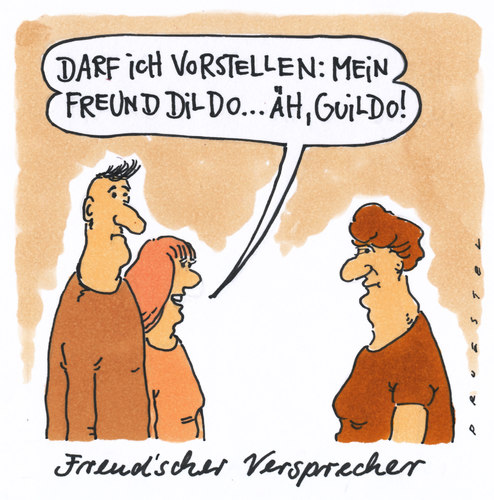
\includegraphics[width=1\textwidth,height=\textheight]{./pictures/freudscher_versprecher_1328535.jpg}}

}

\end{figure}

\emph{Versprecher} (en. speech error, slip of the tongue, sl. jezikovni
spodrsljaj) sind \textbf{unwillkürliche} sprachliche Fehler, die beim
Sprechen unterlaufen und nicht auf organische oder sonstige
gesundheitliche Ursachen zurückgeführt werden können.
\href{https://de.wikipedia.org/wiki/Versprecher}{wikipedia}

Je nach Modalität sind unterscheidbar:\\
\emph{Versprecher, Verschreiber, Vertipper, Verhörer, Verleser,
Vergebärdler}.

Versprecher sind bildungssprachlich auch als \emph{Lapsus linguae}
bekannt.

In den Medien werden (konstruierte) Versprecher gerne satirisch zur
Kritik und Bloßstellung von öffentlich bekannten Personen verwendet.

\begin{figure}

{\centering 

\href{https://www.vn.at/vorarlberg/2022/09/16/freudscher-versprecher.vn}{
\includegraphics[width=1\textwidth,height=\textheight]{./pictures/Europa_von_Leyen_regiert.jpg}}

}

\end{figure}

\emph{Freudsche Versprecher} sind gemäß Leuninger (1993) und Wiedenmann
(1998) keine besondere Versprecherkategorie, da sie wie die übrigen
Versprecher das Ergebnis fehlerhafter Sprachplanung (Sprachausführung)
darstellen und sind daher unter allen Versprecherkategorien zu finden.
Versprecher geben keinen Aufschluss über Unterbewusstes (obwohl dies
früher einmal vermutet wurde).

\hypertarget{definition}{%
\section{Definition}\label{definition}}

Bei Versprechern handelt es sich um Fehlleistungen des Gehirns bei der
Sprachproduktion, die sich auf verschiedenen sprachlichen Ebenen
bemerkbar als antizipatorische oder perseverierende
Serialisierungsfehler machen:

-- \emph{Auslassung} (Elision, Deletion, Omission),\\
- \emph{Hinzufügung} (Intrusion, Epenthese, Addition),\\
- \emph{Ersetzung} (Substitution),\\
- \emph{Vertauschung} (Metathese),\\
- \emph{Kontamination} (Vermischung, Blending).

\begin{figure}

{\centering 

\href{https://www.spreadshirt.de/shop/design/spektakel+farben+wortspiel+freudscher+versprecher+laetzchen-D5c00c8ae5fd3e424dc819325?sellable=yrwD10aLwvs9vJdpgqNV-235-205}{
\includegraphics[width=1\textwidth,height=\textheight]{./pictures/spektakel-farben-wortspiel-freudscher-versprecher-laetzchen.png}}

}

\end{figure}

Versprecher treten bei allen Sprechern \emph{gelegentlich} auf (im
Durchschnitt 1 Versprecher auf 1000 Wörter), häufiger jedoch, wenn sie
nervös, müde, ängstlich oder betrunken sind. Bei Live-Übertragungen in
öffentlichen Medien unterlaufen Laiensprechern und sogar routinierten
Moderatoren häufig Versprecher, weil sie unter \emph{Zeitdruck / Stress}
stehen.

Bei normaler \emph{Sprechgeschwindigkeit} fallen viele Versprecher gar
nicht auf und werden unbewusst \emph{korrigiert}, und zwar sowohl
semantisch als auch grammatisch ( --\textgreater{} Akkomodation).

\begin{center}\rule{0.5\linewidth}{0.5pt}\end{center}

\hypertarget{versprecher-aus-linguistischer-sicht}{%
\section{Versprecher aus linguistischer
Sicht}\label{versprecher-aus-linguistischer-sicht}}

Linguisten, Psycholinguisten und Psychologen sind einerseits daran
interessiert, Versprecher zu \emph{klassifizieren}, andererseits aber
auch daran, die Ursachen für ihr Auftreten zu \emph{erklären}.

Eine der ersten \emph{Versprechersammlungen} wurde von \emph{Meringer}
(1895) angelegt und in einer Studie veröffentlicht (Meringers
Versprechersammlung ist auch in der Datenbank von \emph{Wiedenmann} 1998
zu finden).

\emph{Neuere Erklärungsansätze} gehen von \emph{Sprachplanungsmodellen}
aus, und zwar mit dem Ziel, die Versprecher den vermuteten
\emph{Sprachplanungsebenen} zuzuordnen.

\emph{Sprachplanungsphasen} (nach Leuninger 1996):

\begin{itemize}
\tightlist
\item
  Als erstes kommt die \emph{Botschaft} (message), die einer anderen
  Person mitgeteilt werden soll. Diese Botschaft muss durch das
  Produktionssystem des Sprechers umgesetzt werden und durchläuft dabei
  folgende hypothetischen \emph{Ebenen} (vereinfacht):\\
\item
  eine \emph{prädikative Ebene}, auf der die Bedeutung geplant wird;\\
\item
  eine \emph{positionale Ebene}, auf der die grammatische Form
  entwickelt wird; vermutlich erfolgt auch eine \emph{lexikalische und
  grammatische Kontrolle};\\
\item
  das \emph{Artikulationsprogramm} mit einer \emph{Lautkontrolle}, was
  die grammatisch strukturierte Form schließlich in eine
  \emph{angemessene} \emph{Lautform} bringt, die sprachliche Äußerung.
\end{itemize}

Die Versprecher lassen sich nun diesen Ebenen der Sprachplanung
zuordnen.

Versprecher können nur innerhalb eines sehr \emph{engen zeitlichen
Rahmens} stattfinden, da sie wohl durch Fehler im \emph{Arbeitsspeicher}
des Sprechers zustande kommen (dessen Kapazität scheint für ca. 7 Silben
zu reichen).

\begin{center}\rule{0.5\linewidth}{0.5pt}\end{center}

\hypertarget{klassifizierungen}{%
\section{Klassifizierungen}\label{klassifizierungen}}

Es gibt nur wenige Versprecher, die sich eindeutig in eine einzige
Kategorie einordnen ließen. Die meisten Versprecher fallen daher in mehr
als eine Kategorie. Aus diesem Grund sollte man Vorkommenshäufigkeiten
(Prozentzahlen) für die verschiedenen Versprechertypen mit Vorsicht
genießen. Die verschiedenen Klassifizierungen unterscheiden sich sowohl
methodisch als auch terminologisch.

\hypertarget{leuninger-1993-1996}{%
\subsection{Leuninger (1993, 1996)}\label{leuninger-1993-1996}}

\begin{itemize}
\item
  \emph{Substitutionen}: Ersetzungen aufgrund von Bedeutungs- oder
  Formähnlichkeit. Bei der Ersetzung eines formähnlichen Wortes werden
  strenge Regeln befolgt; so weist das falsche Wort meist die gleiche
  Silbenzahl, gleiche oder gleich empfundene Endungen und Anfangslaute
  etc. wie das Wort auf, das eigentlich geäußert werden sollte.
  Beispiel: „renommiert`` statt „renoviert`` (88). Es entsteht scheinbar
  kein neues Wort, sondern es wird eines durch das andere aufgrund von
  Formähnlichkeit ersetzt.
\item
  \emph{Vertauschungen}, die bei Wörtern meist innerhalb derselben
  Wortart ablaufen. Wörter, Teile von zusammengesetzten Wörtern, Silben
  oder auch Laute tauschen ihren Platz. Beispiel {[}ursprünglich aus
  Rudolf Meringers Corpora: 1895 / 1908{]}: „zwecktischer Prack`` statt
  „praktischer Zweck`` (83).
\item
  Bei \emph{Antizipationen} (Vorwegnahmen) werden sprachliche Einheiten
  in einer Äußerung vorweggenommen. Diese Einheiten können die
  obengenannten Einheiten: Wörter, Wortbestandteile, Lautgruppen/Laute
  sein; Beispiel: „Ich wollte sie stockbrieflich verfolgen lassen``: das
  „o`` aus „verfolgen`` wird (hier ein substitutives Beispiel)
  vorgezogen in der zeitlichen Serialisierung (84).
\item
  \emph{Postpositionen} (Nachklänge, Repetitionen; auch mit dem aus der
  Pathologie stammenden Begriff Perseveration bezeichnet) sind das
  Gegenstück zu den Antizipationen. Hier klingen sprachliche Elemente
  nach, was bedeutet, dass eine Einheit, die zuvor schon geäußert wurde,
  bei der Sprachplanung noch aktiv ist und aus diesem Grund
  fälschlicherweise ein zweites Mal (substitutiv oder aber auch additiv)
  verwendet wird. Hiervon betroffen können alle bereits genannten
  Einheiten sein; Beispiel: „sozialistische Zekten`` für „sozialistische
  Sekten`` (Leuninger 1996: 73).
\item
  \emph{Kontaminationen} von Syntagmen oder Wörtern. Sie gelten als die
  spannendste Versprecherkategorie und treten (sprecherbezogen;
  Versprechen ist idiosynkratisch) auch relativ häufig auf. Hierbei
  vermischen sich zwei konkurrierende Elemente, wobei relevante Teile
  beider Ausdrücke zusammengefügt werden. Beispiel für eine
  Kontamination von Wörtern ist: „Hinwaltspunkt`` für „Hinweis/
  Anhaltspunkt`` (98).
\end{itemize}

Ein \emph{Beispiel für die Zuordnung eines Versprechers} zu einer der
Sprachplanungsebenen: Den Versprecher „\emph{Ich kann nicht über meine
Haut springen}`` interpretiert Leuninger (1993: 164) als
\emph{Kontamination} der Wendungen „\emph{Ich kann nicht über meinen
Schatten springen}`` und „\emph{Ich kann nicht aus meiner Haut}`` und
ordnet ihn der prädikativen Ebene zu, also der Ebene der Sprachplanung,
auf der die Bedeutung einer Äußerung geplant wird. Die zwei an einer
Kontamination beteiligten Einheiten (meist Wörter oder Phrasen) müssen
bei der Sprachplanung beide präsent sein -- sonst könnten sie nicht
miteinander verschmolzen werden.{[}6{]}

Leuninger verweist ferner darauf, dass bei \emph{zweisprachig}
aufwachsenden Kindern auch die Interaktion beider Sprachen zu
Versprechern führen kann.

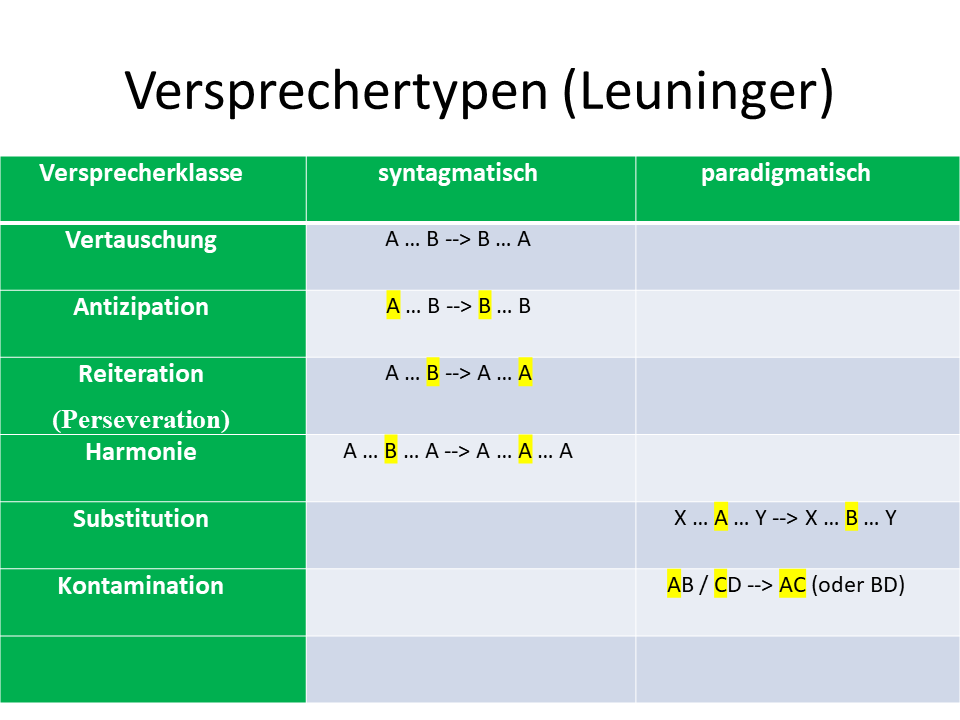
\includegraphics[width=1\textwidth,height=\textheight]{./pictures/Versprechertypen_2.PNG}

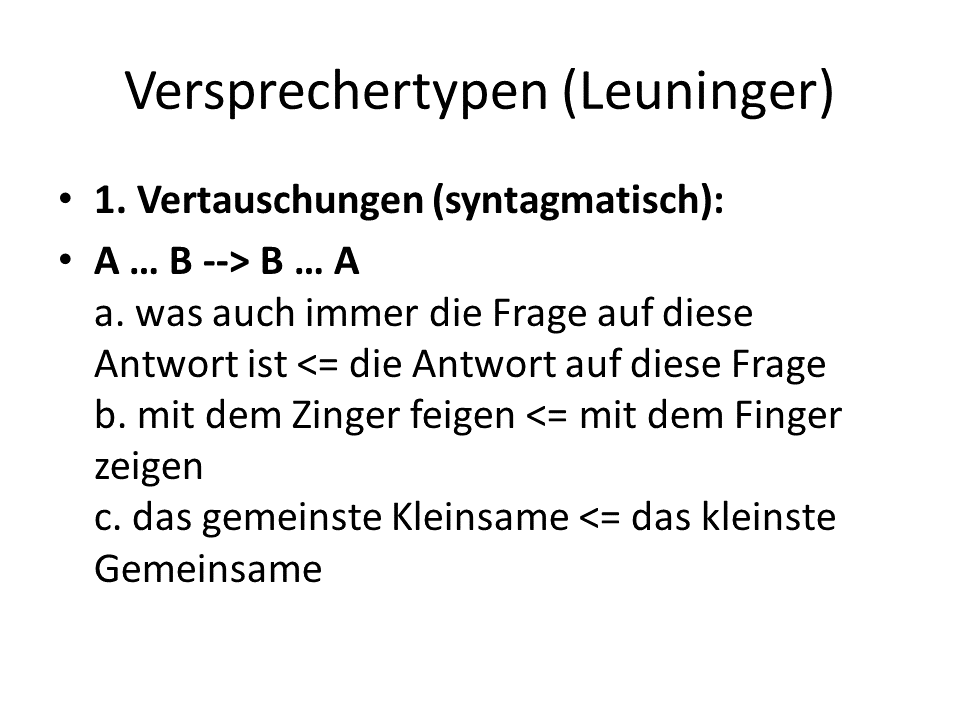
\includegraphics[width=1\textwidth,height=\textheight]{./pictures/Versprechertypen_3.PNG}

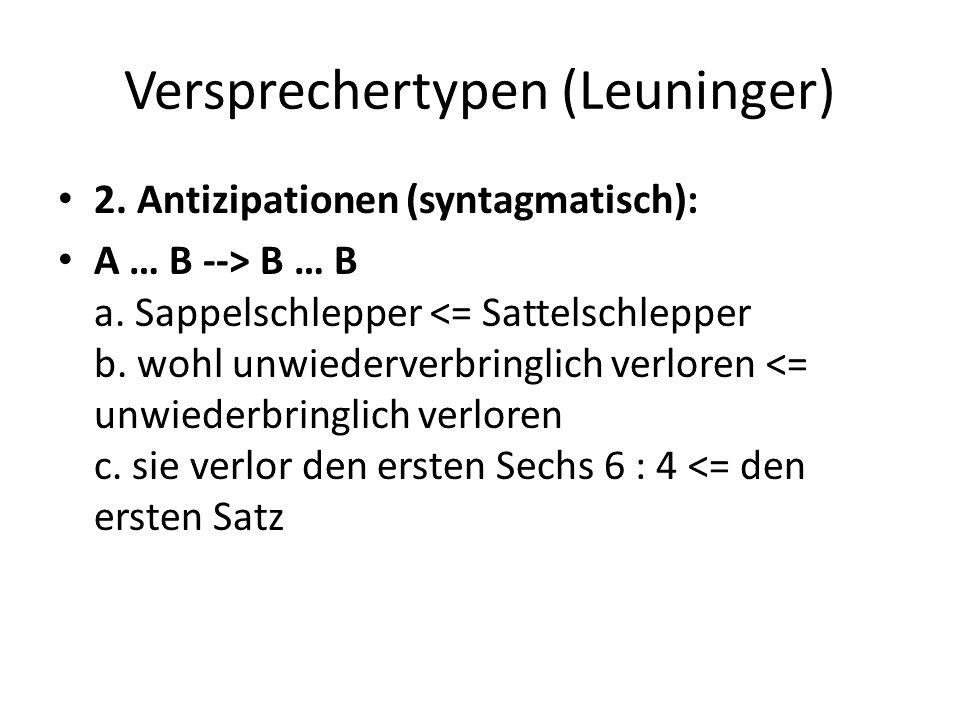
\includegraphics[width=1\textwidth,height=\textheight]{./pictures/Versprechertypen_4.PNG}

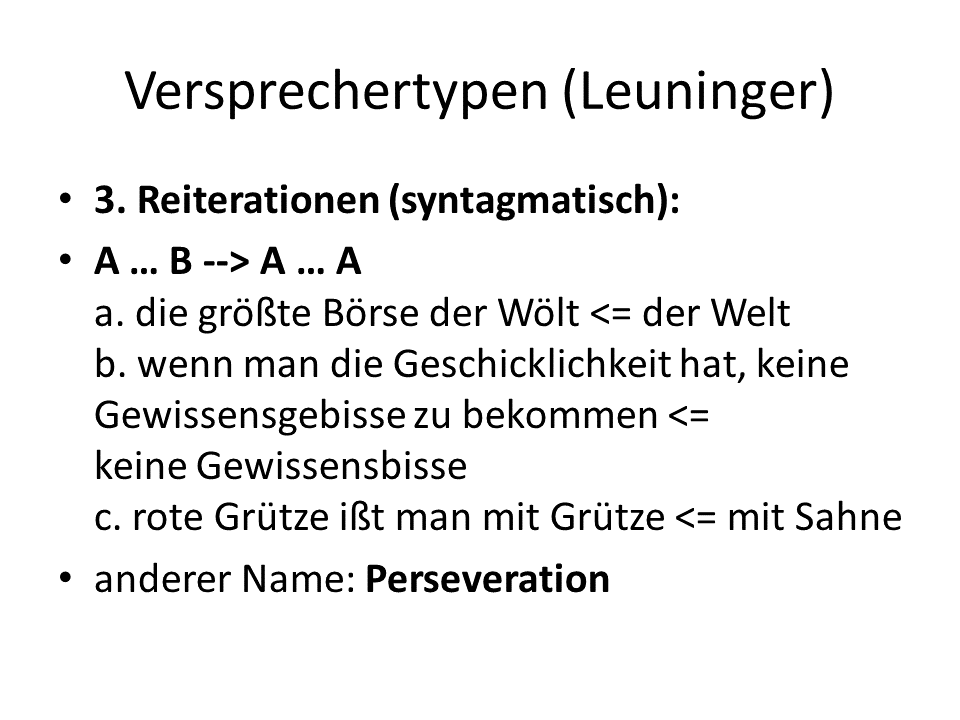
\includegraphics[width=1\textwidth,height=\textheight]{./pictures/Versprechertypen_5.PNG}

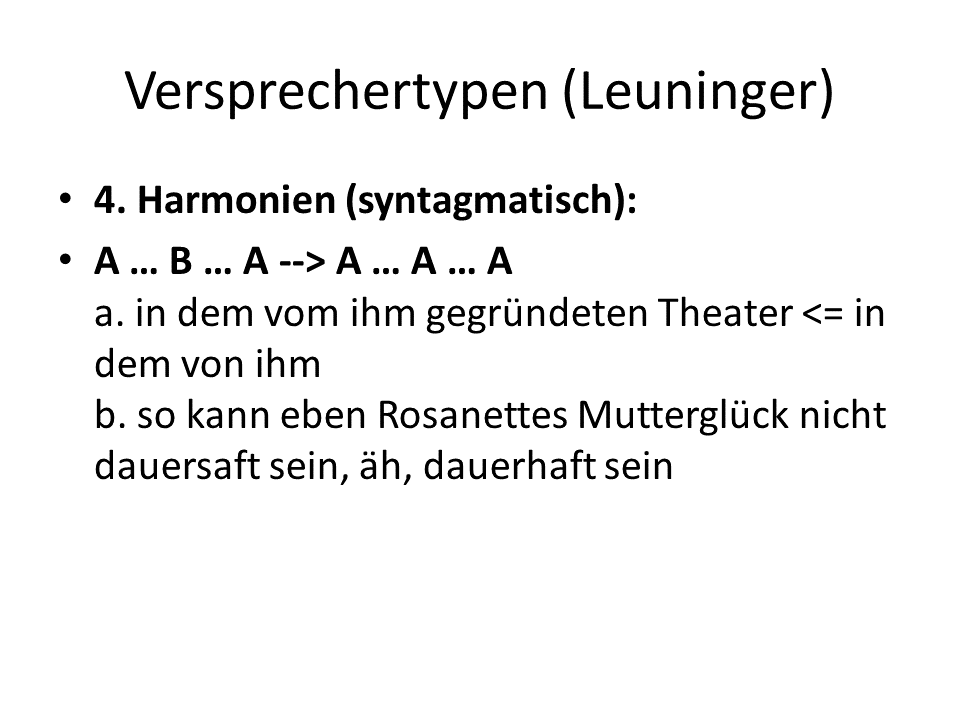
\includegraphics[width=1\textwidth,height=\textheight]{./pictures/Versprechertypen_6.PNG}

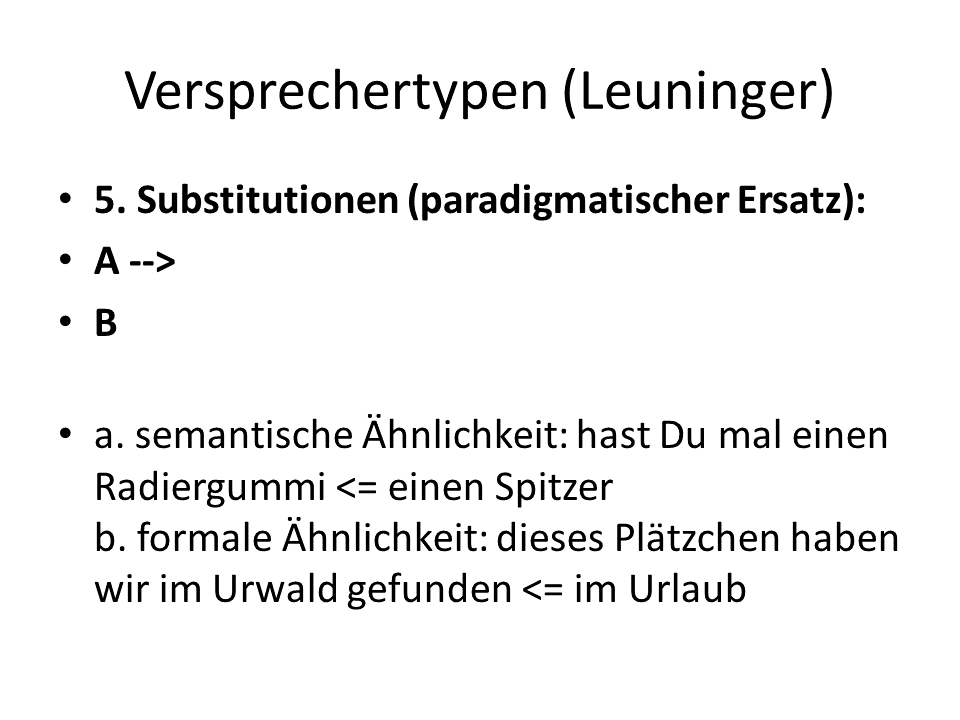
\includegraphics[width=1\textwidth,height=\textheight]{./pictures/Versprechertypen_7.PNG}

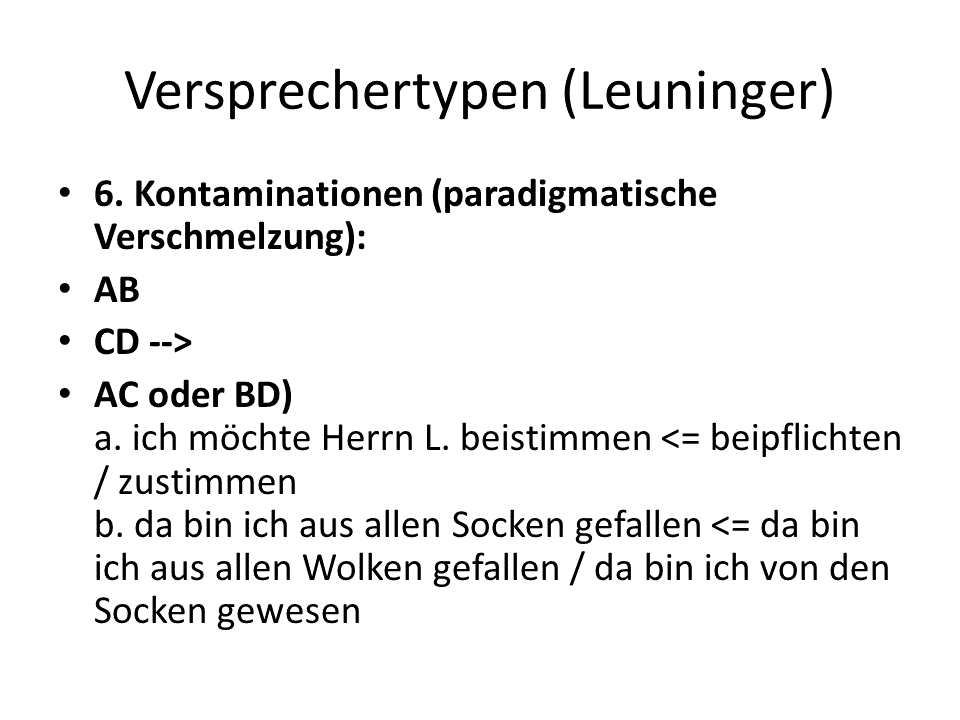
\includegraphics[width=1\textwidth,height=\textheight]{./pictures/Versprechertypen_8.PNG}

\textbf{Versprecherarten} (Beispiele aus einer Präsentation von
\emph{Markus Steinbach}, Uni Mainz):

\begin{itemize}
\tightlist
\item
  \emph{Vertauschung}: Saukramer \textless-- Grausamer\\
\item
  \emph{Antizipation}: ich werde nun zur Abschreitung der Anträge
  schreiten \textless-- zur Abstimmung der Anträge schreiten\\
\item
  \emph{Postposition}: auf das Wohl unseres Chefs aufzustoßen
  \textless-- auf das Wohl unseres Chefs anzustoßen\\
\item
  \emph{Kontamination}: sich verabtschüssen \textless-- sich
  verabschieden/tschüss sagen\\
\item
  \emph{Substitution}: wes Brot ich ess, des Lob ich trink \textless--
  wes Brot ich ess, des Lob ich sing\\
\end{itemize}

\begin{center}\rule{0.5\linewidth}{0.5pt}\end{center}

\hypertarget{klassifizierung-nach-stemberger}{%
\subsubsection{Klassifizierung (nach
Stemberger)}\label{klassifizierung-nach-stemberger}}

Stembergers Klassifikationsschema. Die Tabelle ist nur im Html-Format
sichtbar.

\begin{center}\rule{0.5\linewidth}{0.5pt}\end{center}

\hypertarget{versprechersammlung}{%
\section{Versprechersammlung}\label{versprechersammlung}}

Hier ist eine Versprechersammlung von Studierenden der Universität
Maribor. Die Versprechersammlung ist nur im Html-Format sichtbar.

\hypertarget{klassifizierung-mit-englischen-termini}{%
\section{Klassifizierung mit englischen
Termini}\label{klassifizierung-mit-englischen-termini}}

\href{https://en.wikipedia.org/wiki/Speech_error\#Psycholinguistic_classification}{Wikipedia:
Psycholinguistische Klassifikation der Versprechertypen mit englischen
Termini und Beispielen}

\href{https://en.wikipedia.org/wiki/Speech_error\#Psycholinguistic_classification}{Wikipedia:
Betroffene Segmente oder linguistische Einheiten}

\begin{center}\rule{0.5\linewidth}{0.5pt}\end{center}

\hypertarget{sprachproduktionsmodelle}{%
\section{Sprachproduktionsmodelle}\label{sprachproduktionsmodelle}}

Im Gegensatz zur \emph{Sprachverarbeitung} lässt sich die
\emph{Sprachproduktion} nicht so einfach experimentell untersuchen.

Versprecher sind eine Möglichkeit, Einblick in den
Sprachproduktionsprozess und in den Aufbau des
\emph{Sprachproduktionssystems} im menschlichen Gehirn zu erhalten.

Aus Fehlleistungen sind Rückschlüsse möglich, wie eine fehlerfreie
Sprachproduktion funktioniert und in welchen Phasen des
Sprachproduktionssystems es zu Konflikten zwischen den selbständig
arbeitenden Subsystemen kommt.

\hypertarget{leuningers-modell}{%
\subsection{Leuningers Modell}\label{leuningers-modell}}

\textbf{Leuningers Sprachplanungsmodell} (1993, 1996, 1998), vgl. mit
dem Sprachproduktionsmodell von Garrett (1980) und Fromkin (1973) bei
\href{https://en.wikiversity.org/wiki/Psycholinguistics/Models_of_Speech_Production}{Wikiversity}:

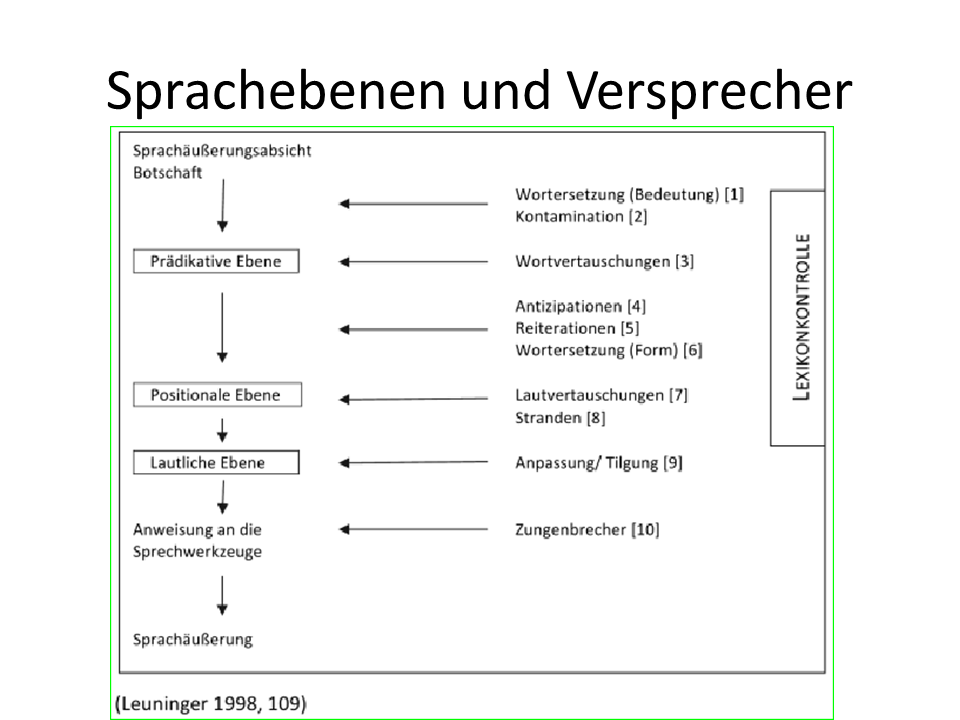
\includegraphics[width=1\textwidth,height=\textheight]{./pictures/Versprechertypen_9.PNG}

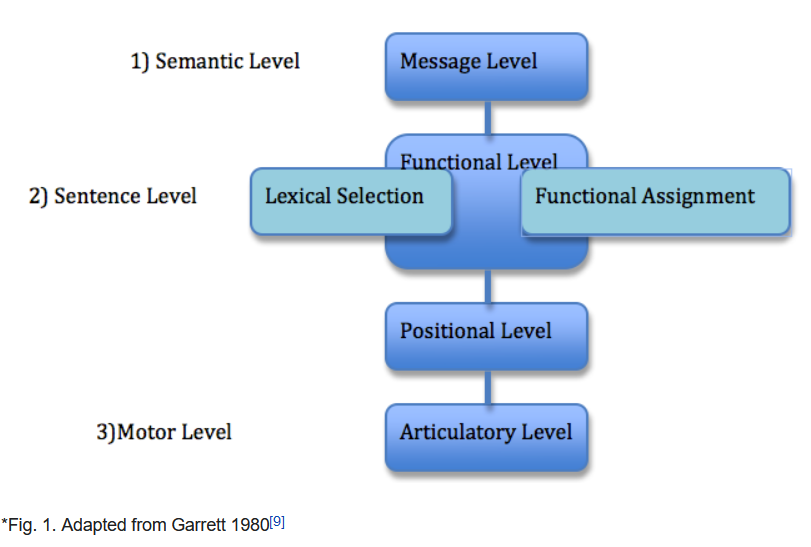
\includegraphics[width=1\textwidth,height=\textheight]{./pictures/Garrett_1980.png}

\textbf{Steinbachs} Darstellung seines Sprachplanungsmodells:

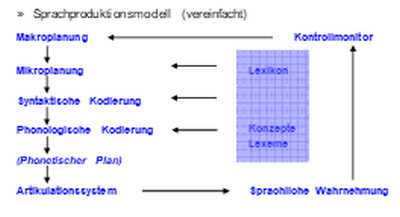
\includegraphics[width=1\textwidth,height=\textheight]{./pictures/Steinbach_8.png}

\hypertarget{sequentielles-modell-bock-levelt}{%
\subsection{Sequentielles Modell (Bock \&
Levelt)}\label{sequentielles-modell-bock-levelt}}

Sprachproduktionsmodell von \textbf{Levelt, Roelofs und Mayer (1999)}:

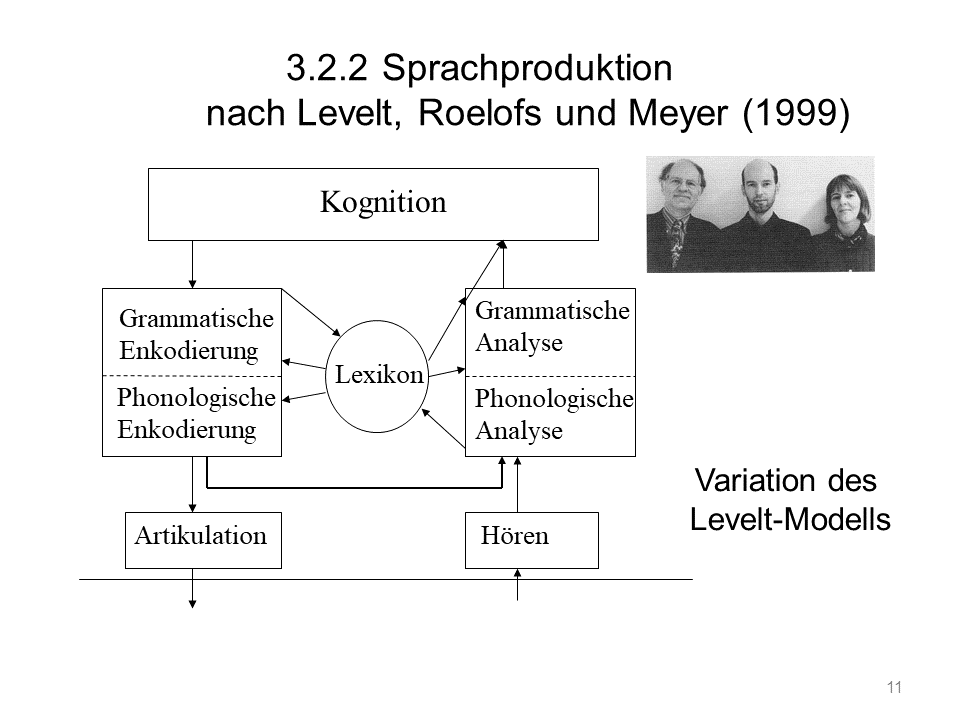
\includegraphics[width=1\textwidth,height=\textheight]{./pictures/Versprechertypen_11.PNG}

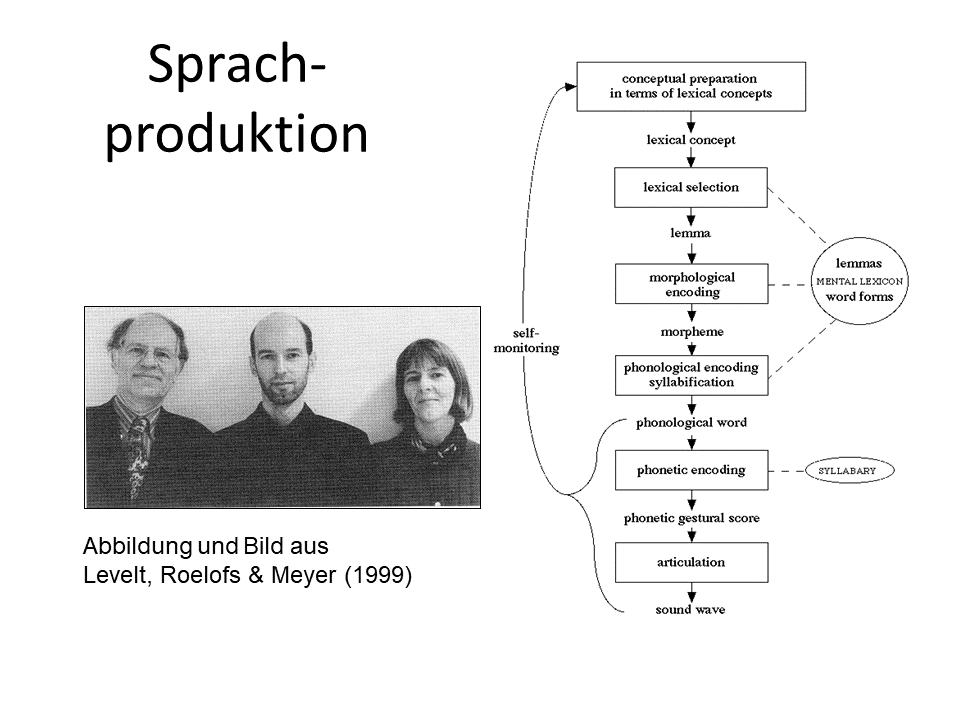
\includegraphics[width=1\textwidth,height=\textheight]{./pictures/Versprechertypen_12.PNG}

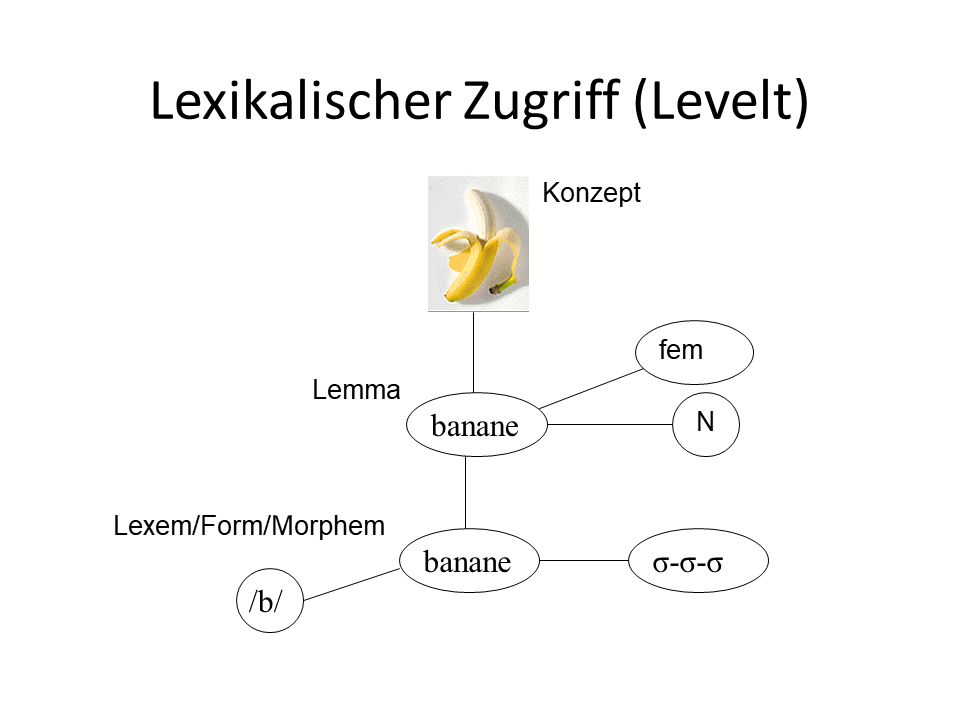
\includegraphics[width=1\textwidth,height=\textheight]{./pictures/Versprechertypen_13.PNG}

\emph{Kritik am Sprachproduktionsmodell} von Levelt, Roelofs \& Mayer:

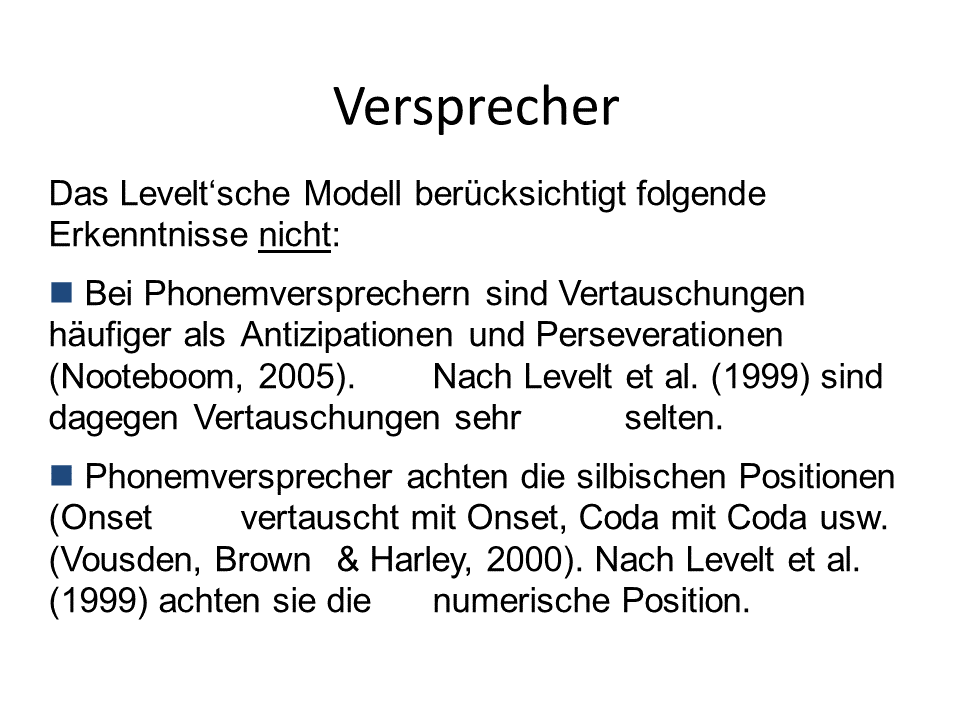
\includegraphics[width=1\textwidth,height=\textheight]{./pictures/Versprechertypen_14.PNG}

\hypertarget{konnektionistische-modell}{%
\subsection{Konnektionistische Modell}\label{konnektionistische-modell}}

Konkurrenzmodell von \emph{Dell (1986)}, ein \textbf{konnektionistisches
Modell} mit Feedback-Schleife: parallele Verarbeitung

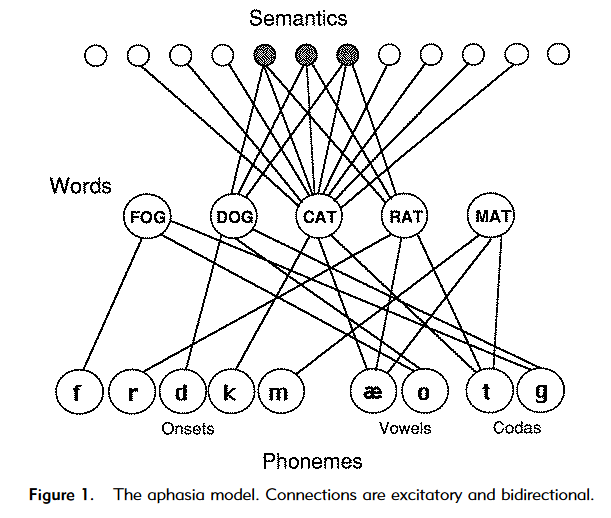
\includegraphics[width=1\textwidth,height=\textheight]{./pictures/Dell_error_model_2.png}

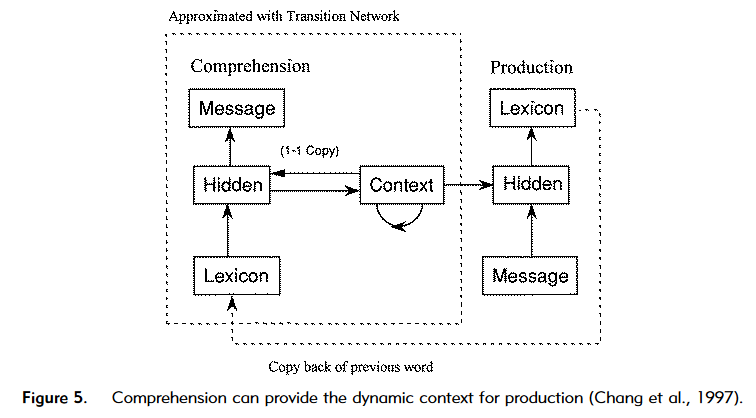
\includegraphics[width=1\textwidth,height=\textheight]{./pictures/Dell_error_model_1.png}

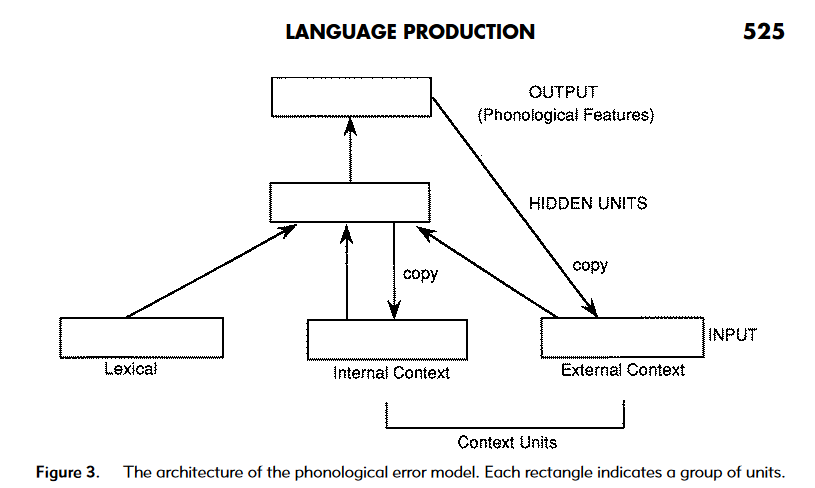
\includegraphics[width=1\textwidth,height=\textheight]{./pictures/Dell_error_model_3.png}

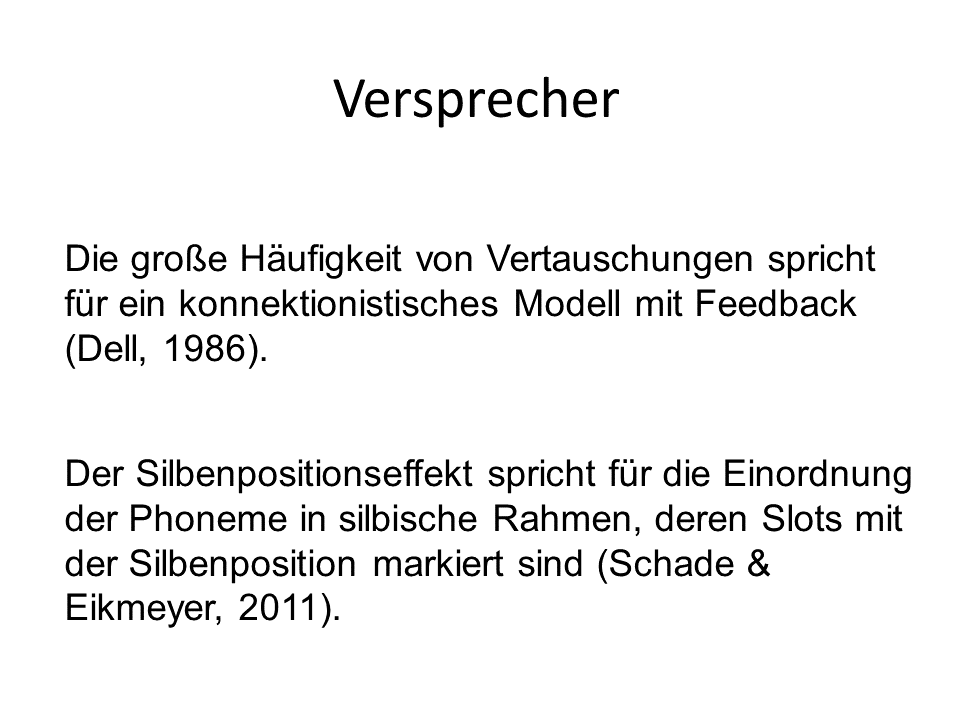
\includegraphics[width=1\textwidth,height=\textheight]{./pictures/Versprechertypen_15.PNG}

\begin{center}\rule{0.5\linewidth}{0.5pt}\end{center}

\hypertarget{stemberger-1993}{%
\subsection{Stemberger (1993)}\label{stemberger-1993}}

\textbf{Einflussfaktoren}

\begin{itemize}
\tightlist
\item
  sprachexterne Faktoren
\item
  sprachinterne Faktoren
\end{itemize}

\hypertarget{sprachexterne-faktoren}{%
\subsubsection{Sprachexterne Faktoren}\label{sprachexterne-faktoren}}

\begin{itemize}
\tightlist
\item
  kognitive Belastung (cognitive load)
\item
  Verdrängung / unterdrückte Gedanken (Freud)
\item
  Sprechtempo
\item
  Müdigkeit
\item
  Betäubung (Alkohol, Drogen)
\end{itemize}

\hypertarget{sprachinterne-faktoren}{%
\subsubsection{Sprachinterne Faktoren}\label{sprachinterne-faktoren}}

Diese Faktoren nehmen Bezug darauf, wie sprachliche Elemente im Gehirn
repräsentiert sind und welche Bestandteile der Botschaft (chunk) bereits
geplant und ausgeführt wurden.

Die meisten Faktoren betreffen die \textbf{Ähnlichkeit} zwischen
sprachlichen Einheiten.

\begin{itemize}
\tightlist
\item
  \textbf{Paralellitäts-Beschränkung}:

  \begin{itemize}
  \tightlist
  \item
    Versprecher betrifft zwei phonologische Elemente in parallelen
    Teilen einer Silbe (beide im Silbenanlaut, beide im Silbenkern oder
    beide im Silbenauslaut);
  \item
    Konsonanten werden durch Konsonanten ausgetauscht, Vokale durch
    Vokale;
  \item
    am stärksten wirkt die Parallelitäts-Beschränkung zwischen Wörtern,
    weniger stark innerhalb eines Wortes.
  \end{itemize}
\item
  \textbf{Silbenstruktur}:

  \begin{itemize}
  \tightlist
  \item
    phonologische Versprecher halten sich an die einzelsprachlichen
    Beschränkungen;
  \item
    stärkere Integration in die Silbenstruktur macht die Veränderung
    eines sprachlichen Element weniger wahrscheinlich;
  \item
    Vokal und auslautende Konsonant(en) bilden gemeinsam den Silbenreim;
    Versprecherrate im Reim ist von der Sonoritäthierarchie abhängig
    (nicht jedoch die Fehlerrate zwischen Anlaut und Vokal);
  \item
    Der Zusammenhalt (Kohesivität) der Silbenbestandteile (z.B. Reim)
    ist auch in Mischkonstruktionen (Kontaminationen, Blends) zu
    beobachten: die Nahtstelle zwischen den beiden Zielwörtern (target
    words) ist gewöhnlich eine Silbengrenze oder liegt zwischen
    Silbenanlaut und Reim, selten zwischen Vokal und Silbenauslaut.
  \end{itemize}
\item
  \textbf{Position im Wort}:

  \begin{itemize}
  \tightlist
  \item
    Anfangsposition im Wort ist wichtig für die Wahrnehmung
    (Perzeption); die größere Fehlerrate bei wort-initialen Konsonanten
    könnte gemäß Dell (1986) an ihrem stärkeren Aktivierungsniveau
    liegen; dieses bahnt konkurrierenden wort-initialen Konsonanten den
    Weg in die Silbe (und eher zu Fehlern);
  \item
    die Position im Wort scheint für das Auftreten von Versprechern
    wichtiger zu sein als die Position in der Silbe (obwohl schwer
    unterscheidbar).
  \end{itemize}
\item
  \textbf{Segment-Ähnlichkeit}:

  \begin{itemize}
  \tightlist
  \item
    Versprecher wahrscheinlicher, wenn phonologische Segmente ähnliche
    Merkmale aufweisen: z.B. /p/ und /k/ eher als /v/ und /k/.
  \end{itemize}
\item
  \textbf{Wiederholungseffekt}:

  \begin{itemize}
  \tightlist
  \item
    Wiederholungseffekt (repetition effect) zeigt die Bedeutsamkeit der
    segmentalen Ähnlichkeit für das Auftreten von Versprechern: wenn ein
    Phonem in zwei benachbarten Wörtern vorkommt, ist ein Fehler
    wahrscheinlich (z.B. Substitution oder Deletion);
  \item
    auch lexikalische Ähnlichkeit kann eine Wiederholung eines Phonems
    herausfordern: wenn zwei Wörter im Satz dasselbe Phonem enthalten,
    dann ist eine Veränderung (Substitution, Addition, Deletion)
    wahrscheinlicher. Dies scheint auch davon abzuhängen, wie stark die
    Ähnlichkeit der phonologischen Elemente in zwei Wörtern (in
    parallelen Silbenpositionen) ist. Die interagierender Wörter gehören
    oft auch zu derselben Wortklasse (z.B. beide sind Verben, beide
    Substantive).
  \end{itemize}
\item
  \textbf{Parallele morphologische Struktur}:

  \begin{itemize}
  \tightlist
  \item
    Präfixe interagieren gewöhnlich mit Präfixen, Suffixe mit Suffixen
    und Infixe mit Infixen;
  \item
    Enkodierung von Bedeutungen ist jedoch in den Sprachen sehr
    unterschiedlich.
  \end{itemize}
\item
  \textbf{Frequenz (Häufigkeit)}:

  \begin{itemize}
  \tightlist
  \item
    mehr Fehler mit seltener vorkommenden sprachlichen Elementen;
  \item
    Frequenz eines Lemmas korreliert mit lexikalischen Versprechern,
    aber auch mit morphologischen und phonologischen;
  \item
    die Häufigkeit eines phonoligischen Elements beeinflusst die
    phonologische Fehlerrate;
  \item
    sowohl Typenfrequenz (d.h. die Häufigkeit verschiedener Wortformen)
    als auch Tokenfrequenz (Gebrauchshäufigkeit einer Wortform) sind von
    Bedeutung für die Fehlerrate;
  \item
    die Typen- und Tokenfrequenz von Phrsenstrukturen mag auch eine
    Rolle spielen bei syntaktischen Fehlern.
  \end{itemize}
\item
  \textbf{Markiertheit (oder: Natürlichkeit)}:

  \begin{itemize}
  \tightlist
  \item
    von Jakobson (1943) vorgeschlagen: markierte sprachliche Elemente
    zeigen die Tendenz, von weniger markierten (unmarkierten) ersetzt zu
    werden (z.B. im kindlichen Spracherwerb; Aphasie).
  \end{itemize}
\item
  \textbf{Neigung zur Hinzufügung (Addition Bias)}:

  \begin{itemize}
  \tightlist
  \item
    in kontextuell bedingten Fehlern (syntagmatischen Fehlern) sind
    Hinzufügungsfehler wesentlich häufiger als Tilgungsfehler;
  \item
    in nicht-kontextuell bedingten Fehlern (paradigmatischen Fehlern)
    sind dagegen eher Tilgungen zu beobachten.
  \end{itemize}
\item
  \textbf{Distanz}:

  \begin{itemize}
  \tightlist
  \item
    geringere Distanz ermöglicht eher Versprecher: in phonologischen
    Fehlern stehen die betroffenen Konsonanten gewöhnlich weniger als
    sieben Wörter oder sieben Silben auseinander;
  \item
    ob Wörter in derselben syntaktischen Phrase auftreten; meist kommen
    zwei interagierende Wörter in derselben übergeordneten Phrase (major
    syntactic phrase) vor;
  \item
    interagierende Wörter in demselben Satz.
  \end{itemize}
\item
  \textbf{Neigung zur Authentizität (Lexical Bias)}:

  \begin{itemize}
  \tightlist
  \item
    phonologische Versprecher sehen gewöhnlich wie richtige Wörter in
    einer Sprache aus, seltener nicht wohlgeformt gemäß einer Sprache.
  \end{itemize}
\item
  \textbf{Stärke (magnitude)}:

  \begin{itemize}
  \tightlist
  \item
    die Faktoren werden in Verwechslungsfehlern (Metathese, exchange
    error) verstärkt;
  \item
    die Faktoren haben einen größeren Effekt auf weniger übliche
    Versprechertypen.
  \end{itemize}
\end{itemize}

\begin{center}\rule{0.5\linewidth}{0.5pt}\end{center}

\hypertarget{betroffene-sprachebenen}{%
\subsection{Betroffene Sprachebenen}\label{betroffene-sprachebenen}}

Beispiele aus einer Präsentation von \emph{Markus Steinbach} (Uni
Mainz).

\textbf{Phonologische Versprecher}\\
(1) mein Kralli putzt \textless-- mein Pulli kratzt\\
(2) da haben mir die Zie geknittert \textless-- da haben mir die Knie
gezittert\\
(3) Stöhnsteuerkarte \textless-- Lohnsteuerkarte\\
(4) eine Cole Dosa \textless-- eine Dose Cola\\
(5) schlecken sie den Stüssel ins Loch \textless-- stecken sie den
Schlüssel ins Loch\\
(6) ich komme vorgen Vormittag \textless-- ich komme morgen Vormittag\\
(7) wieso ist schon wieder der Kapierer kaputt \textless-- der Kopierer
kaputt\\
(8) der Dichter und sein Henker \textless-- der Richter und sein
Henker\\

\textbf{Morphologische Versprecher}\\
(1) buddhistische Standesamt \textless-- statistisches Bundesamt\\
(2) es wird hinten ein unselbständiges Element angefixt, ein Suffix
\textless-- es wird hinten ein unselbständiges Element angefügt, ein
Suffix\\
(3) Es wird wieder alles irgendwo hochsterilisiert \textless- es wird
wieder alles irgendwo hochstilisiert\\
(4) die gängige Ausrede für Herr \textless-- die gängige Anrede für
Herr\\

\textbf{Morphosyntaktische Versprecher}\\
(1) da plötzlich stürzt aus einem Haus mit fliegenden Weibern ein Haar
heraus \textless-- \ldots{} mit fliegenden Haaren ein Weib heraus\\
(2) es gibt Formen von Kriminalität, die importiert zu sein scheint
\textless-- die importiert zu sein scheinen\\
(3) ein Ende der Unruhen sind nicht abzusehen \textless-- ein Ende der
Unruhen ist nicht abzusehen\\
(4) für jedes geäußerte Wort müssten dann eine Mehrzahl von Wörtern
geäußert werden \textless-- für jedes geäußerte Wort müsste dann
\ldots{}\\

\textbf{Semantische Versprecher}\\
(1) sich verabtschüssen \textless-- sich verabschieden/tschüss sagen\\
(2) das Buch hat auch mehrere Auflagen erlitten, erfahren mehrere
Auflagen erfahren\\
(3) als ich auf die Geburt kam \textless-- als ich auf die Welt
kam/geboren wurde\\
(4) ich bin fast aus allen Socken gefallen \textless-- ich bin fast aus
allen Wolken gefallen/von den Socken sein\\
(5) das ist wirklich ein dickes Stück \textless-- ein starkes Stück/ein
dickes Ding\\

\begin{center}\rule{0.5\linewidth}{0.5pt}\end{center}

\hypertarget{versprecherkorrekturen}{%
\subsection{Versprecherkorrekturen}\label{versprecherkorrekturen}}

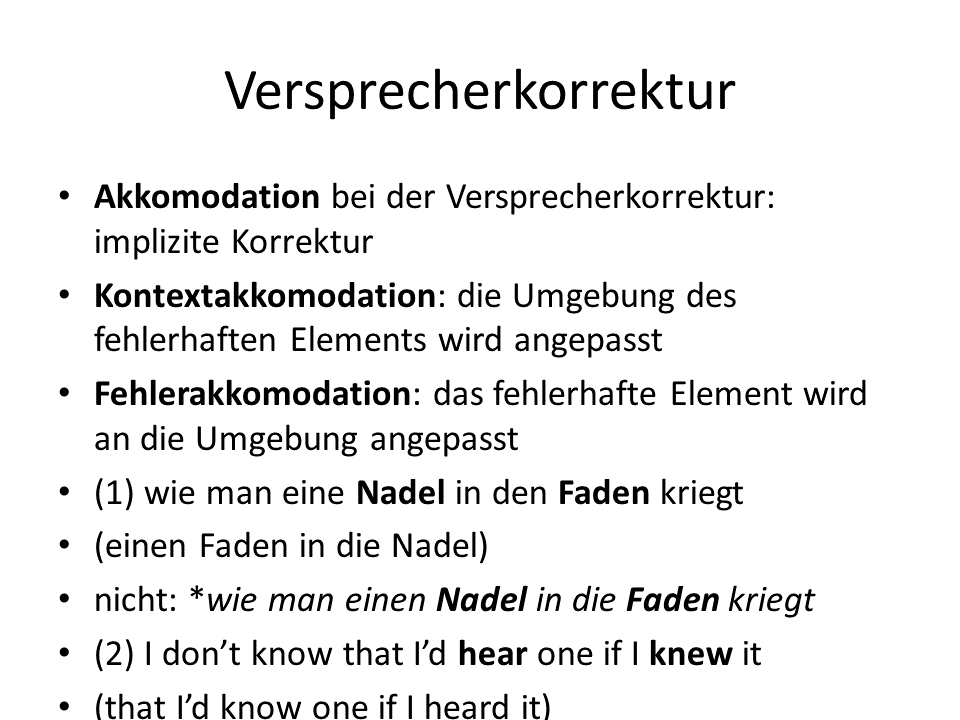
\includegraphics[width=1\textwidth,height=\textheight]{./pictures/Versprechertypen_10.PNG}

Fehlerakkomodation nach sprachlichen Ebenen geordnet (Markus Steinbach,
Mainz):

\textbf{Morphologische Akkommodation}\\
(1) Männer können nämlich noch trink-en, wenn sie was ge-fahr-en haben
\textless-- (noch fahren, wenn sie was getrunken haben)\\
nicht: \emph{nämlich noch trunken, wenn sie was gefahren haben\\
(2) ge-monat-ete Arbeit-en \textless-- (gearbeitete Monat-e)\\
nicht: }Arbeit-e\\
(3) dass er mit dem Zug zieh-t \textless-- (mit der Masse zieht)\\
nicht: *dass er mit der Zieh zieh\\

\textbf{Morphosyntaktische Akkommodation}\\
(1) irgendwie habe ich heute eine Zunge im Knoten \textless-- einen
Knoten in der Zunge\\
nicht: \emph{irgendwie habe ich heute einen Zunge in der Knoten\\
(2) bis er es bei dir abhol-t \textless-- bis du es bei ihm abhol-st\\
nicht: }bis ihm es bei du abholst\\

\textbf{Lexikalische Akkommodation}\\
(1) Stöhnsteuerkarte \textless-- Lohnsteuerkarte\\
nicht: *Stohnsteuerkarte\\

\begin{center}\rule{0.5\linewidth}{0.5pt}\end{center}

Helen Leuninger: Reden ist Schweigen, Silber ist Gold. Gesammelte
Versprecher. 2. Auflage. Ammann, Zürich 1993. ISBN 3-250-10209-1.

Helen Leuninger: Danke und Tschüss fürs Mitnehmen. Gesammelte
Versprecher und eine kleine Theorie ihrer Korrekturen. Ammann, Zürich
1996. ISBN 3-250-10323-3 (beide Bücher von Leuninger enthalten auch eine
linguistische Theorie der Versprecher auf der Grundlage eines von ihr
entworfenen Sprachplanungsmodells).

Rudolf Meringer, Karl Mayer: Versprechen und Verlesen. Eine
psychologisch-linguistische Studie. Göschen'sche Verlagshandlung,
Stuttgart 1895. (Neudruck: A. Cutler, D. Fay (eds.): Amsterdam Studies
in the Theory and History of Linguistic Science II: Classics in
Psycholinguistics, Vol. 2. Benjamins, Amsterdam 1978).

Nora Wiedenmann: Versprecher. Phänomene und Daten {[}1--78;
Bibliographie zum Versprechen und zu verwandten Phänomenen: 79--110;
Appendix: 1--265{]}. Mit Materialien auf Diskette. Wissenschaftsverlag
Edition Praesens, Wien 1998. ISBN 3-901126-91-0.

Joseph P. Stemberger (1993)

\part{Normabweichungen und Normwandel}

\hypertarget{sec-spracherwerb}{%
\chapter{Fehler im Spracherwerb}\label{sec-spracherwerb}}

Fehler in Zweit- und Fremdsprache

\hypertarget{sec-medien}{%
\chapter{Normabweichungen in den neuen Medien}\label{sec-medien}}

\hypertarget{sec-multikulti}{%
\chapter{Multikulturelle Sprachvarietäten}\label{sec-multikulti}}

Kiezdeutsch als Beispiel für Abweichungen von der standardsprachlichen
Norm mit der Entwicklung einer varietätenspezifischen Grammatik.

\hypertarget{sec-gender}{%
\chapter{Gendergerechte Sprache}\label{sec-gender}}

Fehler und Abweichungen beim Bezug auf verschiedene Geschlechter,
insbesondere bei der Vermeidung des generischen Maskulinums.

\bookmarksetup{startatroot}

\hypertarget{abschlieuxdfende-bemerkungen}{%
\chapter{Abschließende Bemerkungen}\label{abschlieuxdfende-bemerkungen}}

Einige Hinweise für \emph{\texttt{selbständige}} Textanalysen. 🤗

\{\{ \textless{} include \_WM\_Presentation.qmd \textgreater{} \}\}

\hypertarget{fontawesome}{%
\section{Fontawesome}\label{fontawesome}}

In the terminal use:\\
quarto install quarto-ext/fontawesome

This extension folder has to be installed in every project.

After installation, use curly braces to include fa icons / or use html
code (e.g.~copy free icons from https://fontawesome.com , namely:
https://fontawesome.com/start).

\faIcon{envelope} - the code for an envelope

\faIcon{facebook} - the code for brands like facebook

For icon-styling go to https://github.com/quarto-ext/fontawesome:

\faIcon{windows}

On https://fontawesome.com/docs, there is information on how to change
the color of the icons, e.g.~in the Styling section, Basics.

{ }

Rotated icons:

Possible to include animated icons:

\hypertarget{callout-types}{%
\section{Callout Types}\label{callout-types}}

\begin{tcolorbox}[enhanced jigsaw, titlerule=0mm, arc=.35mm, breakable, opacitybacktitle=0.6, title=\textcolor{quarto-callout-note-color}{\faInfo}\hspace{0.5em}{Note}, colframe=quarto-callout-note-color-frame, leftrule=.75mm, rightrule=.15mm, coltitle=black, colbacktitle=quarto-callout-note-color!10!white, bottomtitle=1mm, left=2mm, colback=white, toptitle=1mm, bottomrule=.15mm, toprule=.15mm, opacityback=0]

Note that there are five types of callouts, including: \texttt{note},
\texttt{warning}, \texttt{important}, \texttt{tip}, and
\texttt{caution}.

\end{tcolorbox}

\begin{tcolorbox}[enhanced jigsaw, titlerule=0mm, arc=.35mm, breakable, opacitybacktitle=0.6, title=\textcolor{quarto-callout-tip-color}{\faLightbulb}\hspace{0.5em}{Tip With Caption / Tipp mit Titel}, colframe=quarto-callout-tip-color-frame, leftrule=.75mm, rightrule=.15mm, coltitle=black, colbacktitle=quarto-callout-tip-color!10!white, bottomtitle=1mm, left=2mm, colback=white, toptitle=1mm, bottomrule=.15mm, toprule=.15mm, opacityback=0]

This is an example of a callout with a caption.

\end{tcolorbox}

\begin{tcolorbox}[enhanced jigsaw, titlerule=0mm, arc=.35mm, breakable, opacitybacktitle=0.6, title=\textcolor{quarto-callout-important-color}{\faExclamation}\hspace{0.5em}{Important}, colframe=quarto-callout-important-color-frame, leftrule=.75mm, rightrule=.15mm, coltitle=black, colbacktitle=quarto-callout-important-color!10!white, bottomtitle=1mm, left=2mm, colback=white, toptitle=1mm, bottomrule=.15mm, toprule=.15mm, opacityback=0]

Das ist wichtig.

\end{tcolorbox}

\begin{tcolorbox}[enhanced jigsaw, titlerule=0mm, arc=.35mm, breakable, opacitybacktitle=0.6, title=\textcolor{quarto-callout-warning-color}{\faExclamationTriangle}\hspace{0.5em}{Warning}, colframe=quarto-callout-warning-color-frame, leftrule=.75mm, rightrule=.15mm, coltitle=black, colbacktitle=quarto-callout-warning-color!10!white, bottomtitle=1mm, left=2mm, colback=white, toptitle=1mm, bottomrule=.15mm, toprule=.15mm, opacityback=0]

Warning

\end{tcolorbox}

\begin{tcolorbox}[enhanced jigsaw, titlerule=0mm, arc=.35mm, breakable, opacitybacktitle=0.6, title=\textcolor{quarto-callout-caution-color}{\faFire}\hspace{0.5em}{Expand To Learn About Collapse}, colframe=quarto-callout-caution-color-frame, leftrule=.75mm, rightrule=.15mm, coltitle=black, colbacktitle=quarto-callout-caution-color!10!white, bottomtitle=1mm, left=2mm, colback=white, toptitle=1mm, bottomrule=.15mm, toprule=.15mm, opacityback=0]

This is an example of a `folded' caution callout that can be expanded by
the user. You can use \texttt{collapse="true"} to collapse it by default
or \texttt{collapse="false"} to make a collapsible callout that is
expanded by default.

\end{tcolorbox}

\hypertarget{diagrammer-mermaid}{%
\section{DiagrammeR mermaid}\label{diagrammer-mermaid}}

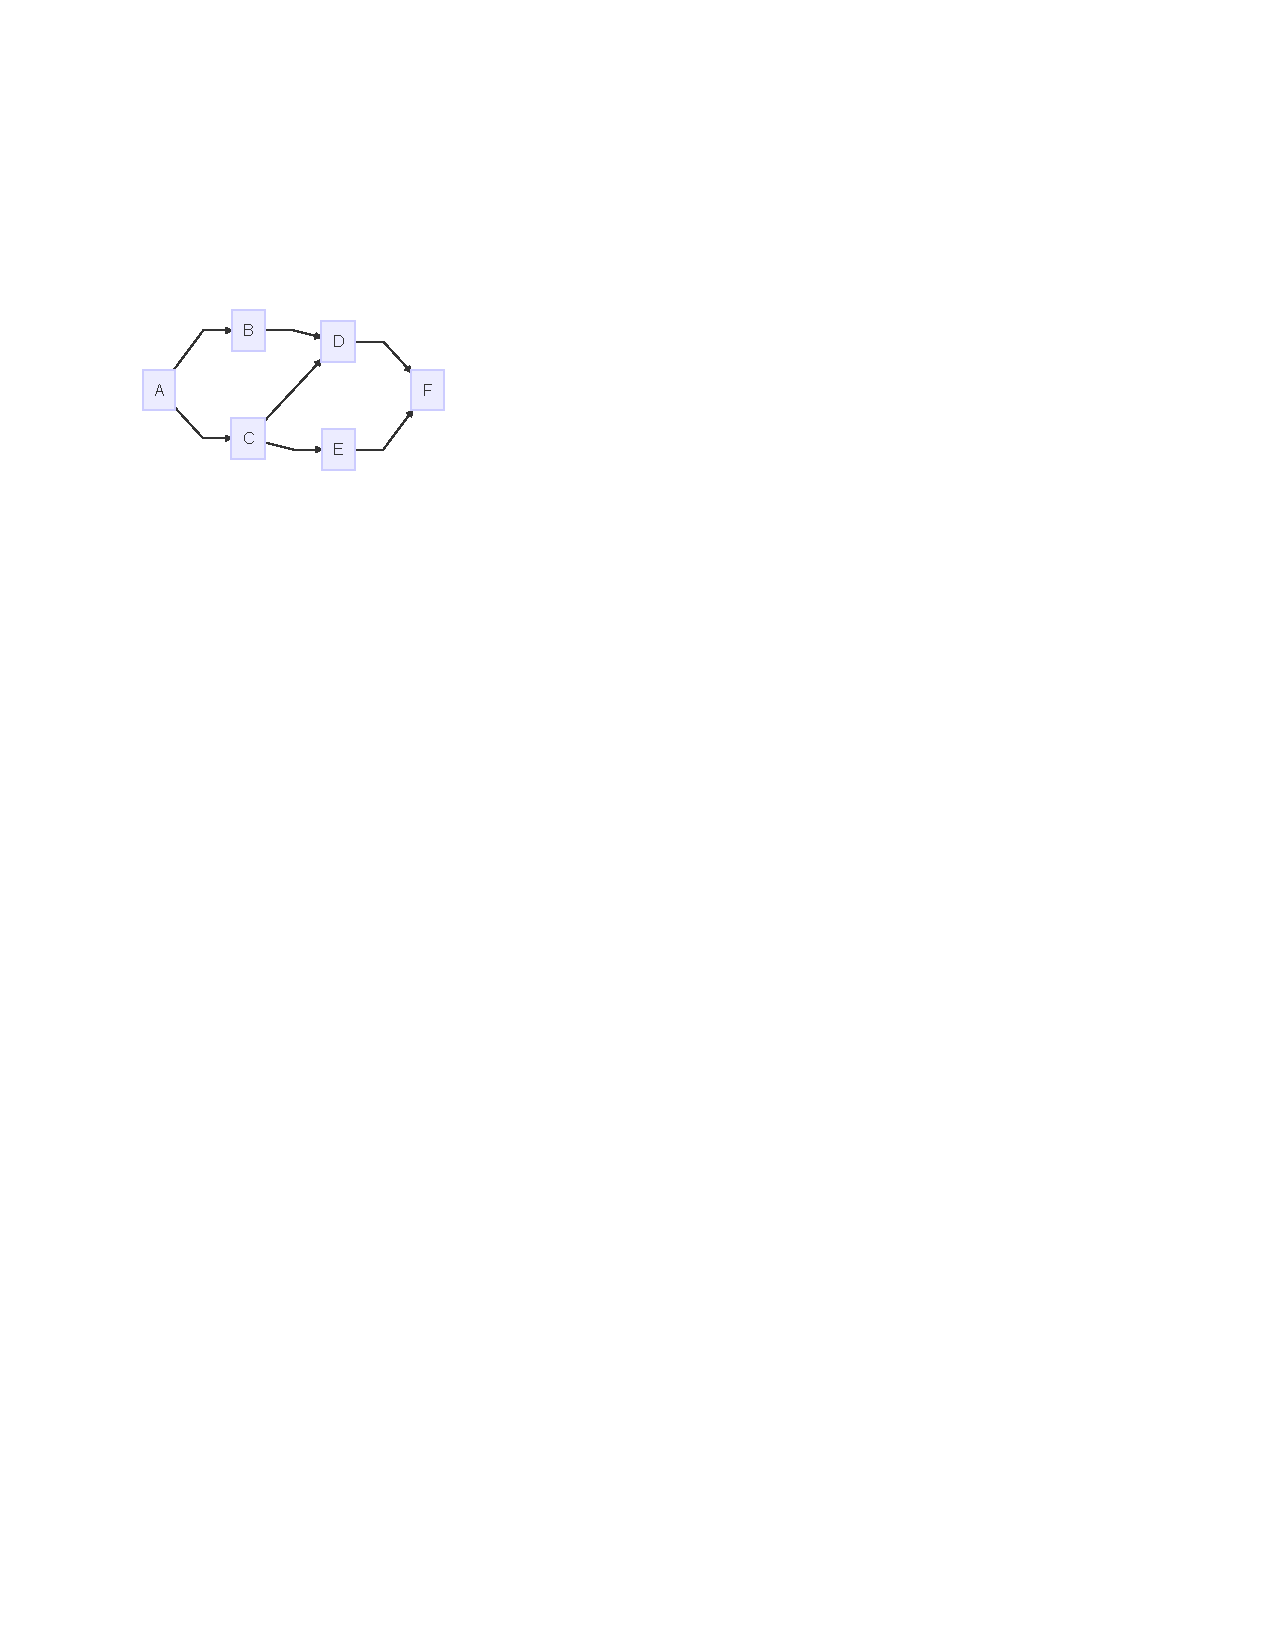
\includegraphics{./summary_files/figure-pdf/unnamed-chunk-1-1.pdf}

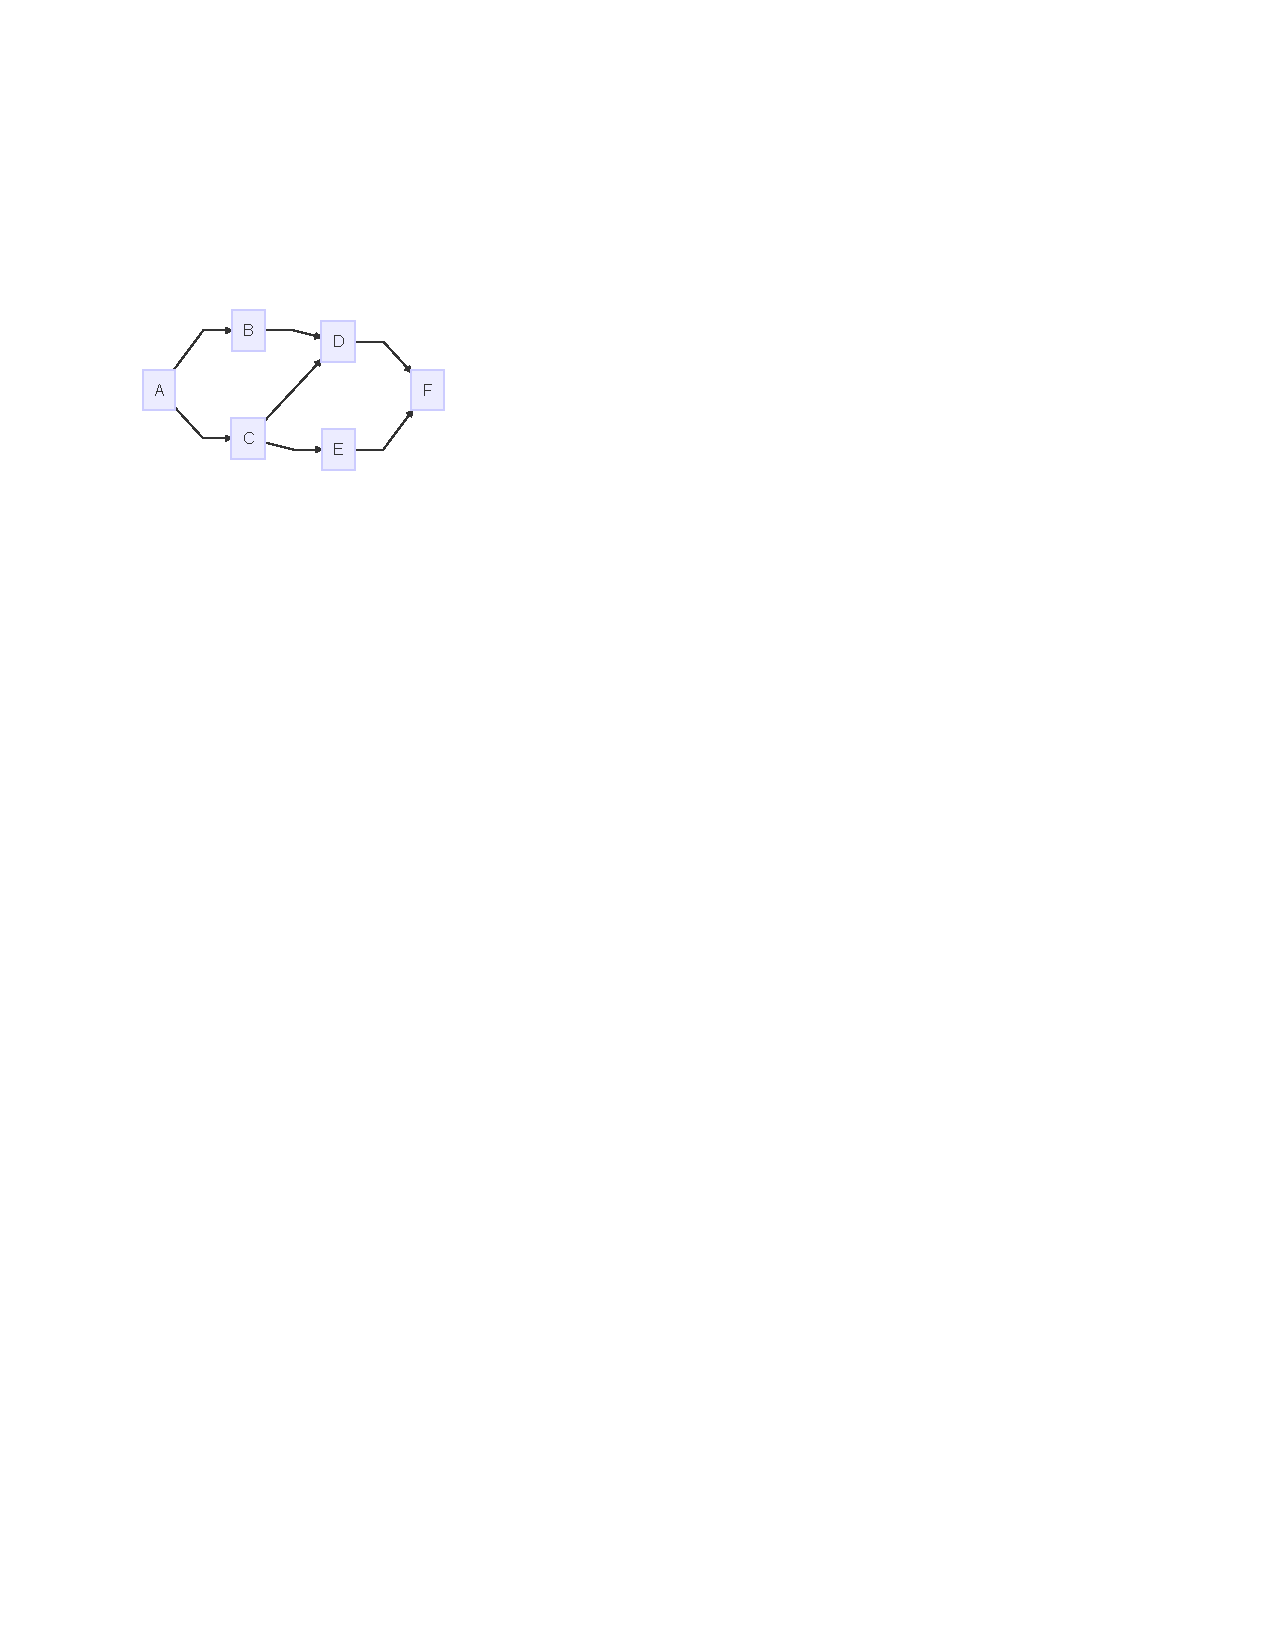
\includegraphics{./summary_files/figure-pdf/unnamed-chunk-2-1.pdf}

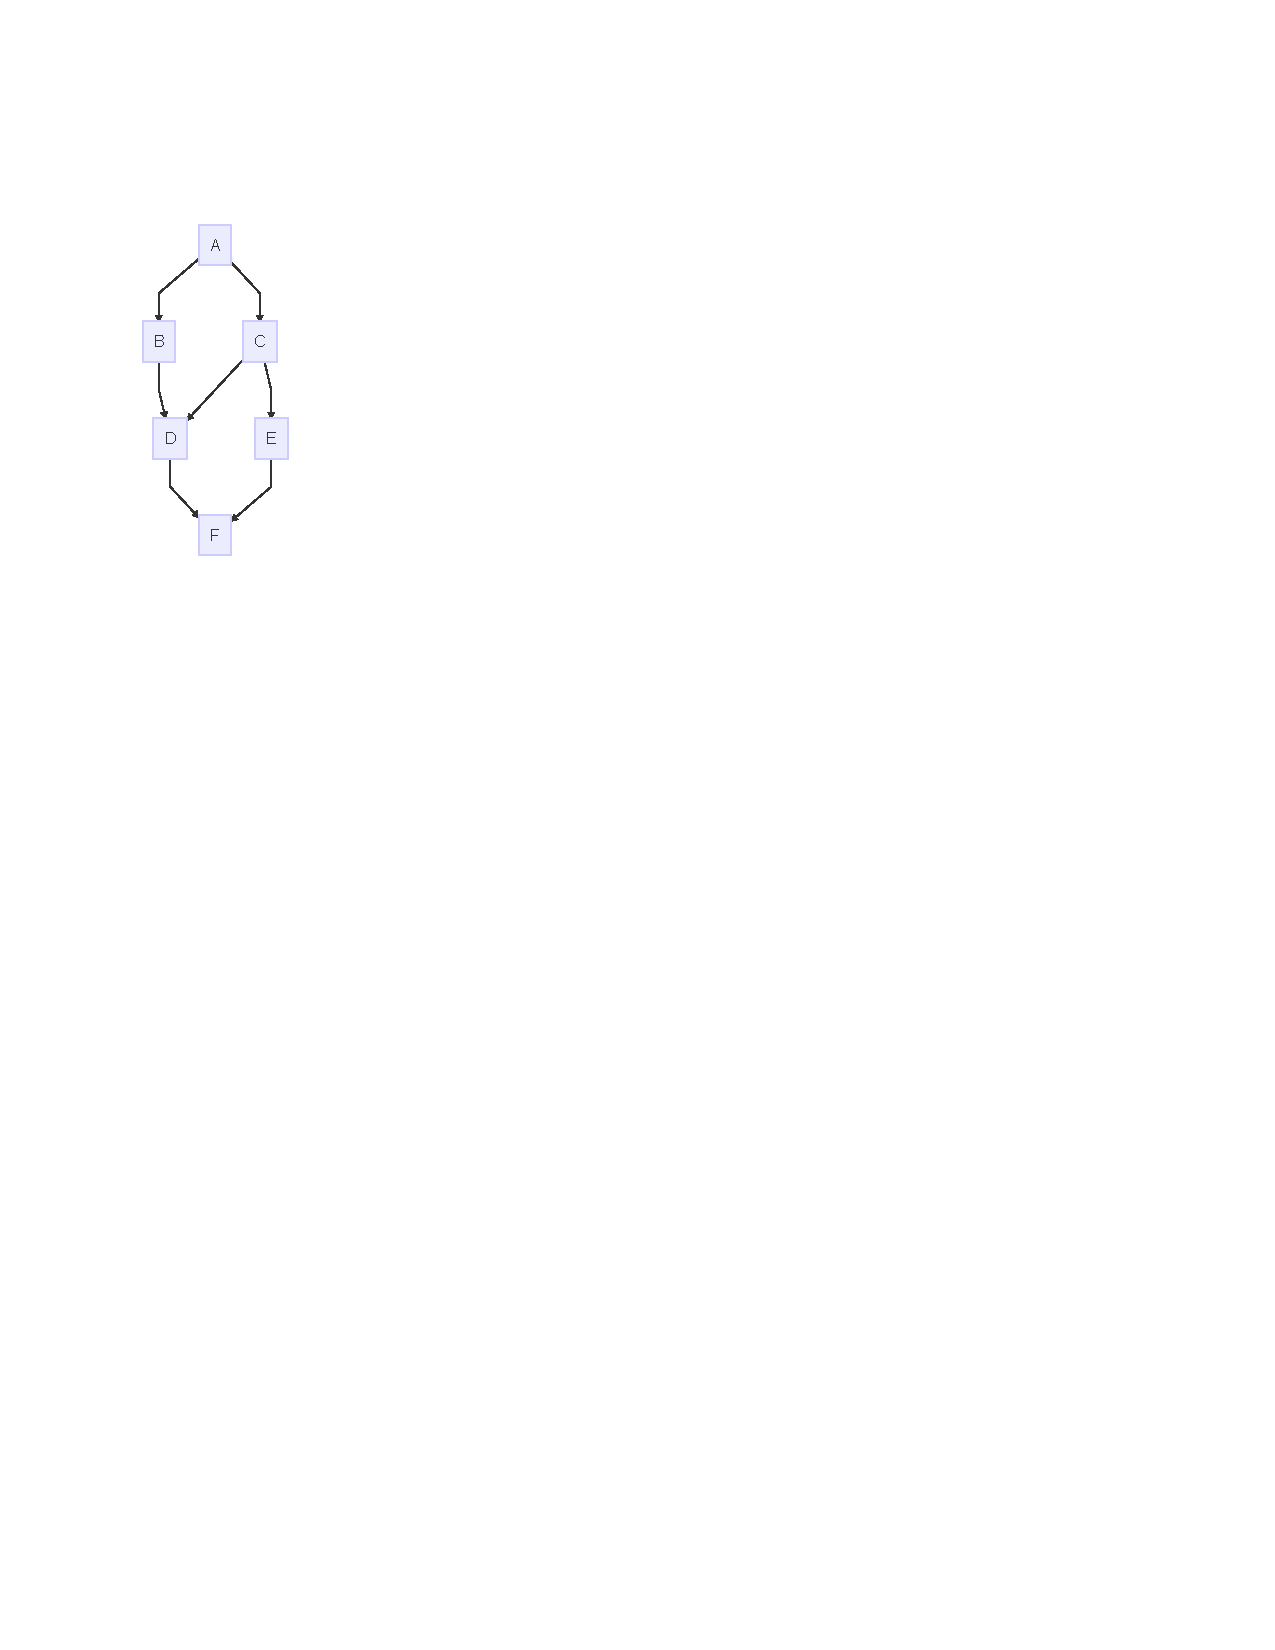
\includegraphics{./summary_files/figure-pdf/unnamed-chunk-3-1.pdf}

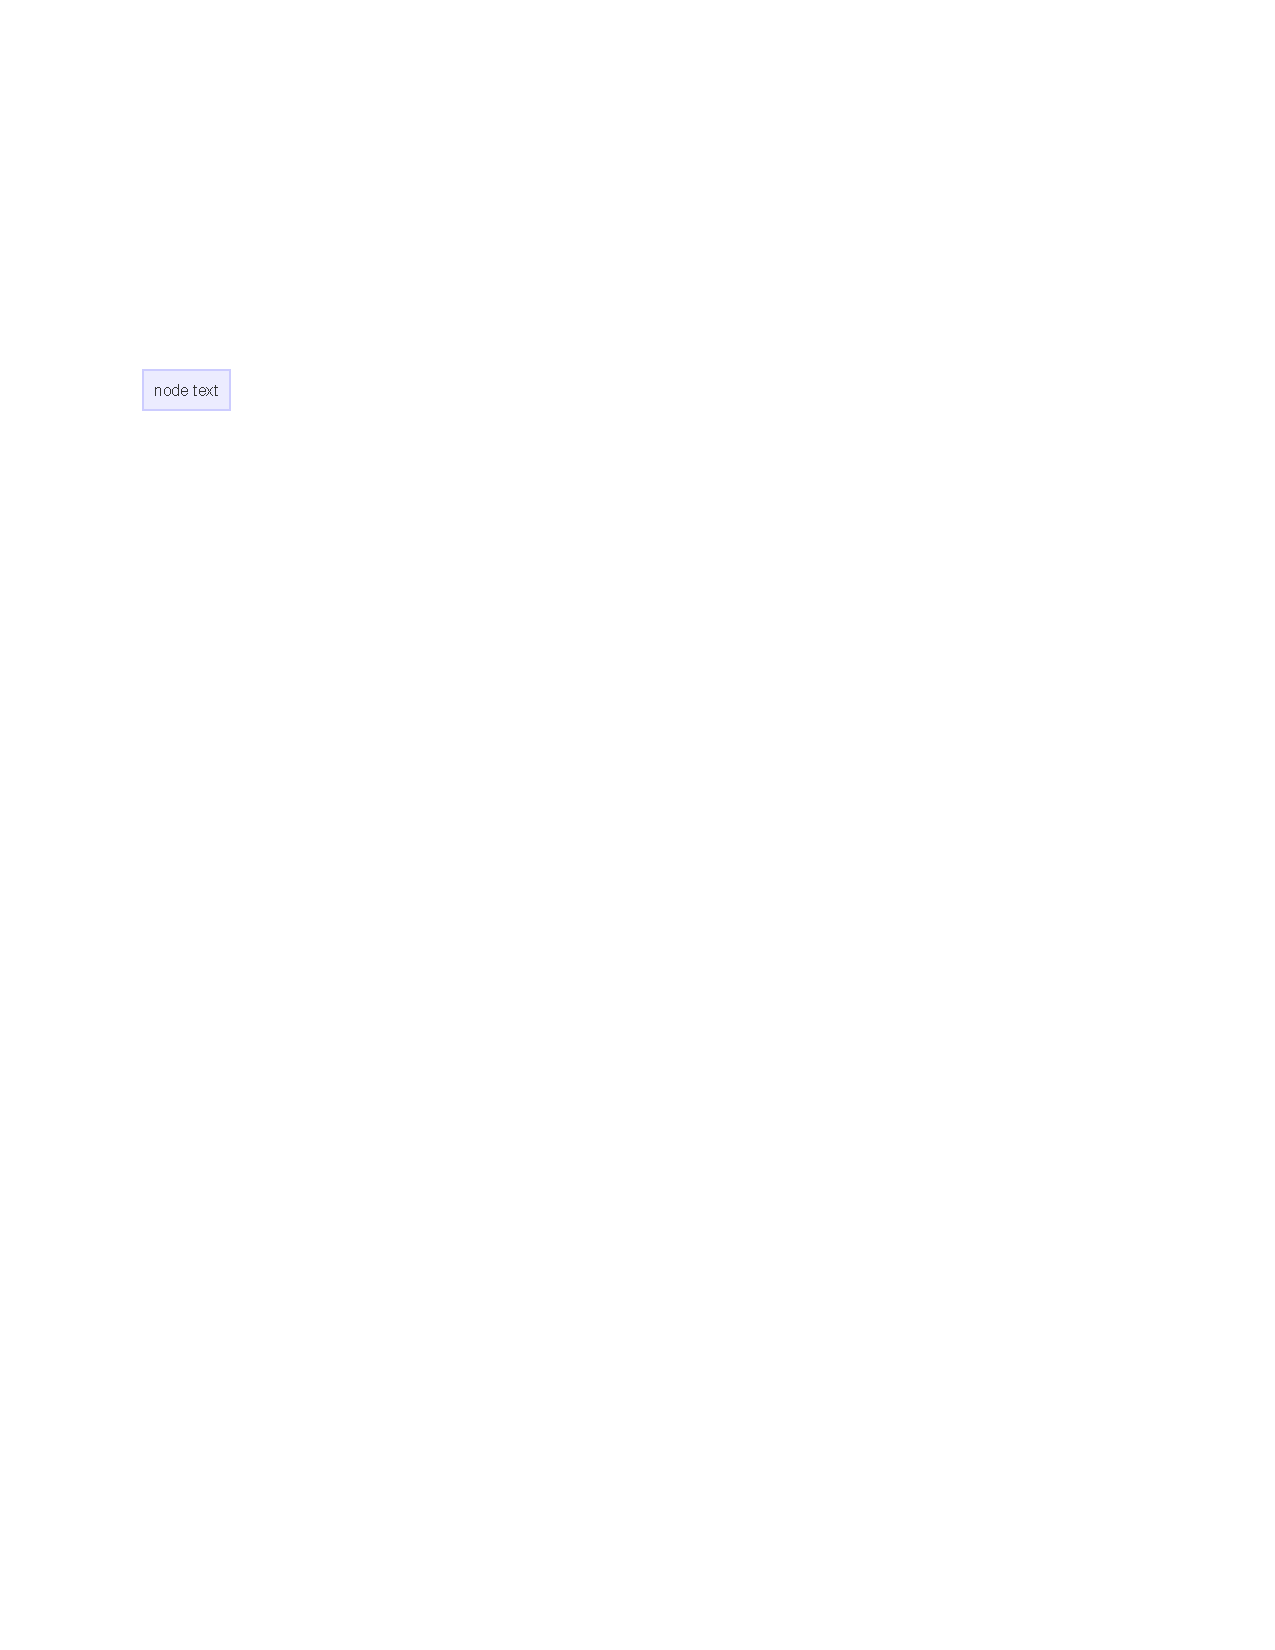
\includegraphics{./summary_files/figure-pdf/unnamed-chunk-4-1.pdf}

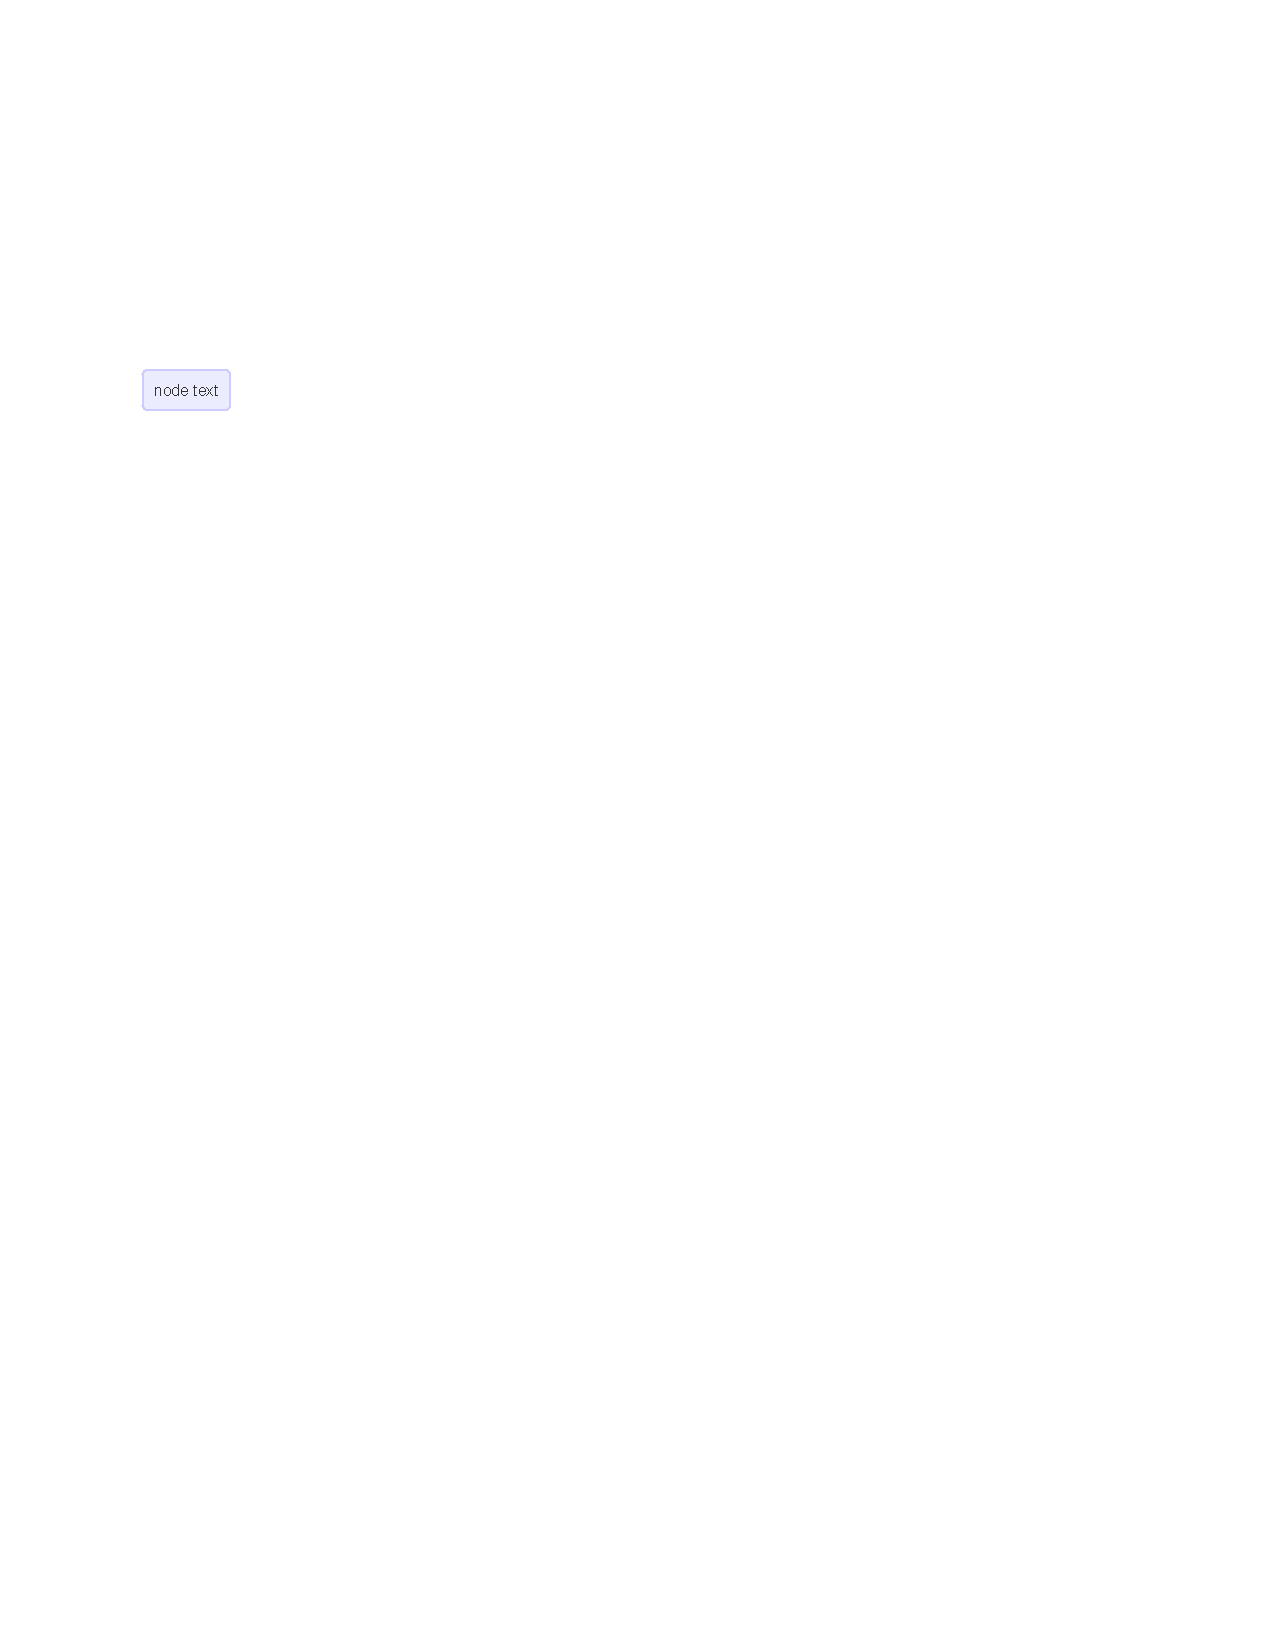
\includegraphics{./summary_files/figure-pdf/unnamed-chunk-4-2.pdf}

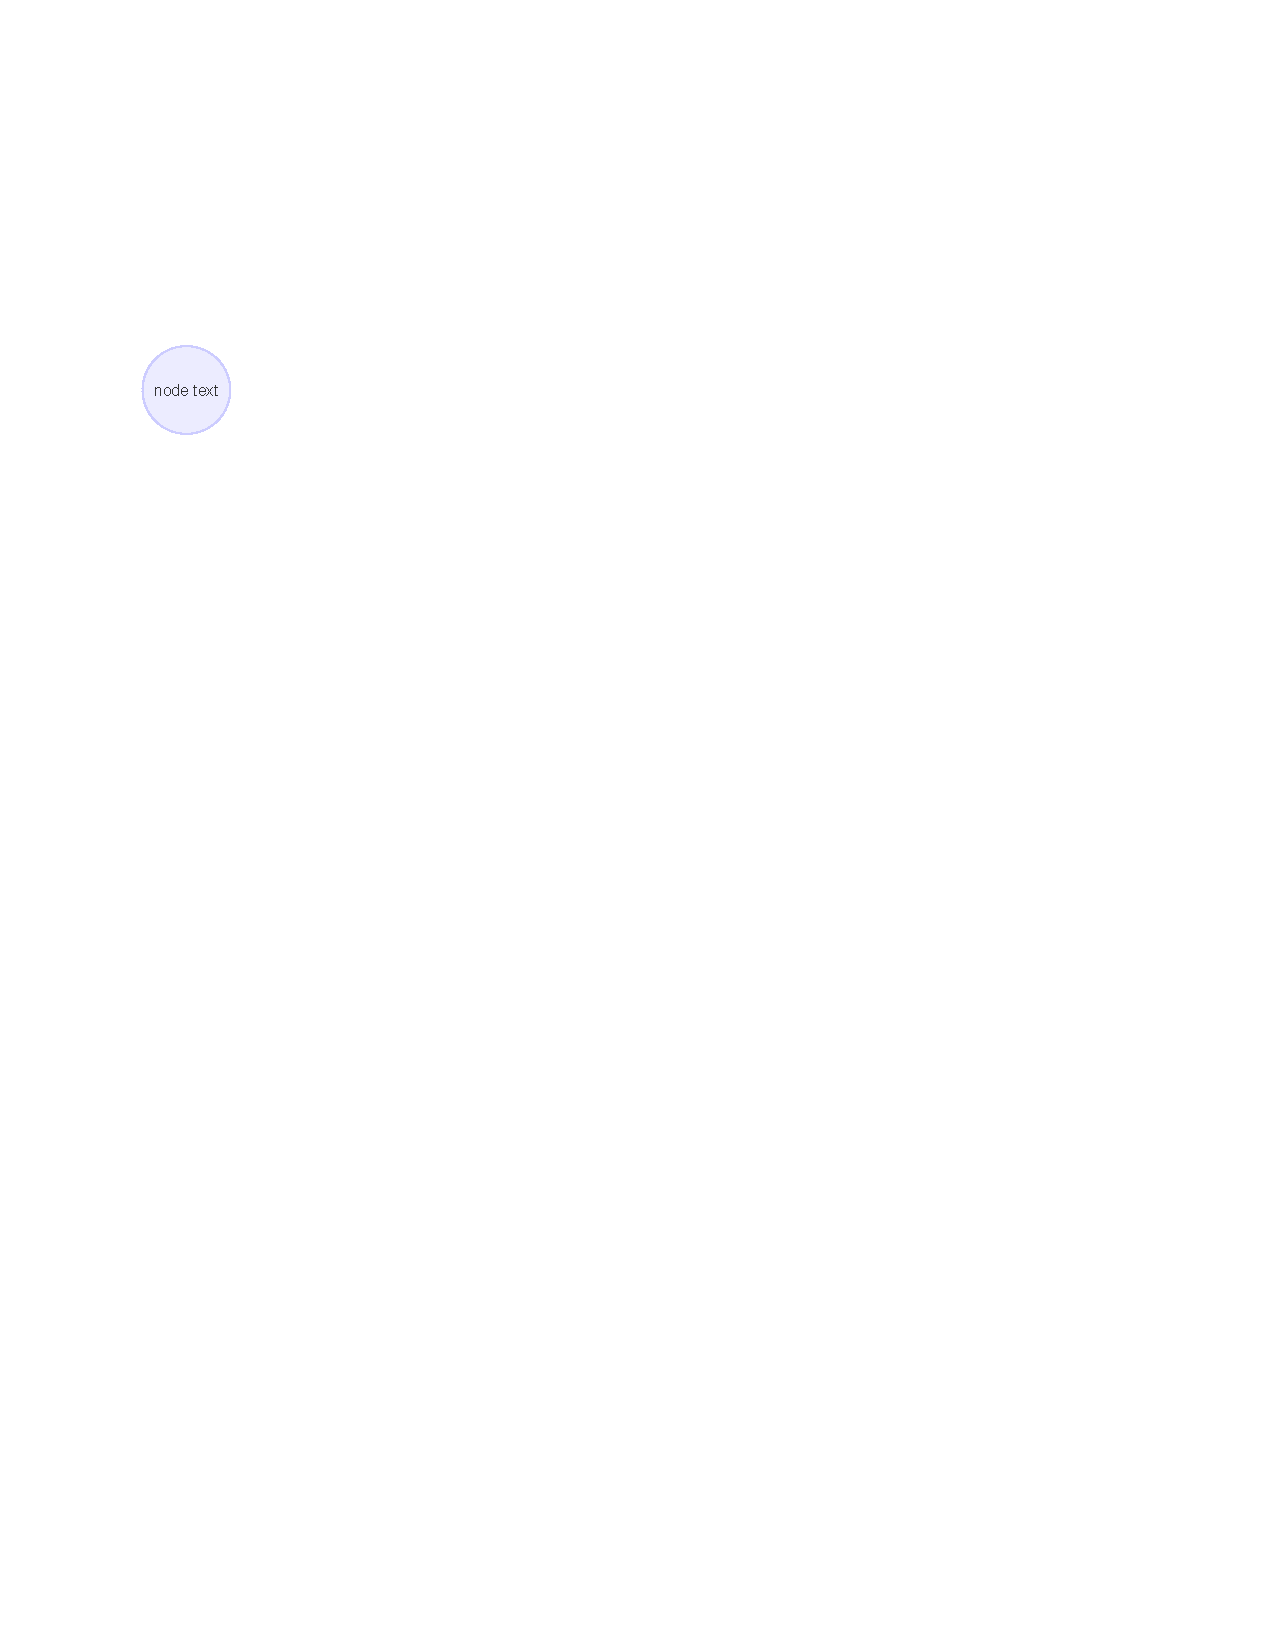
\includegraphics{./summary_files/figure-pdf/unnamed-chunk-4-3.pdf}

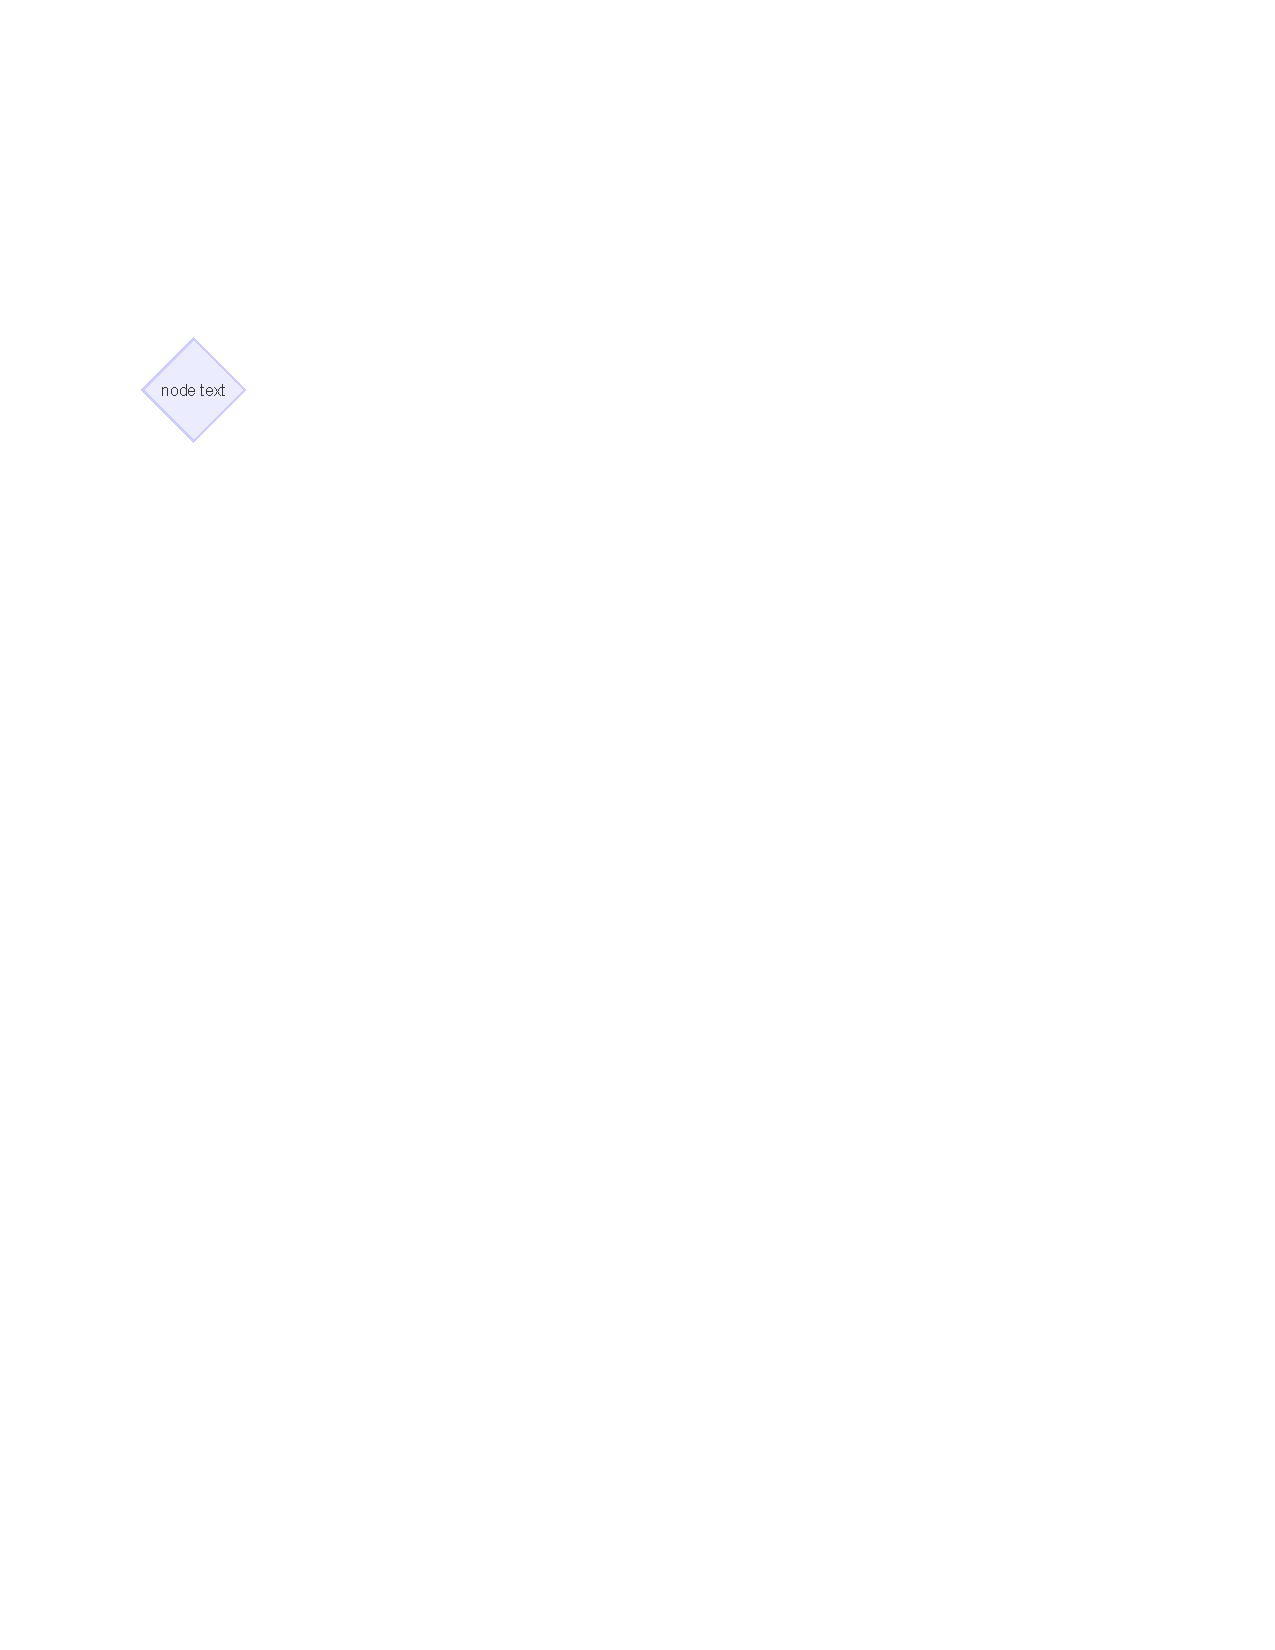
\includegraphics{./summary_files/figure-pdf/unnamed-chunk-4-4.pdf}

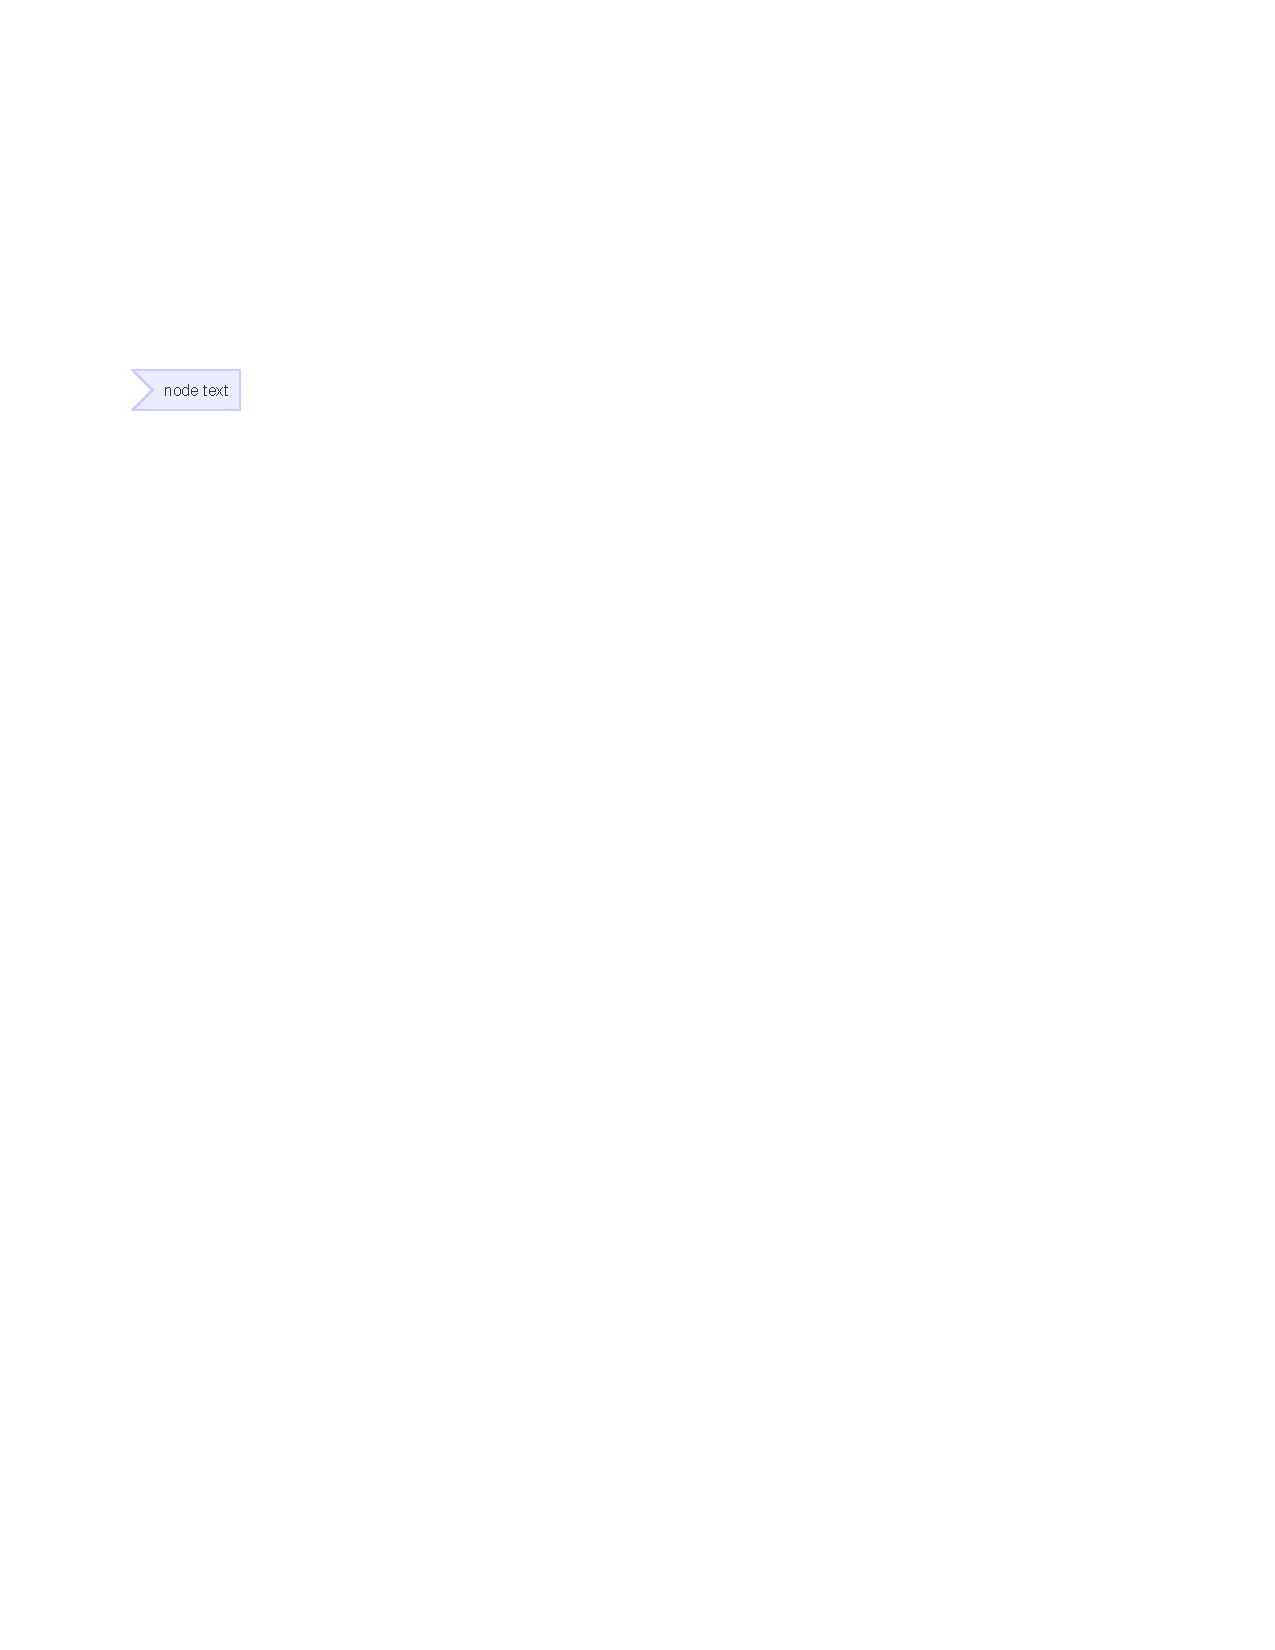
\includegraphics{./summary_files/figure-pdf/unnamed-chunk-4-5.pdf}

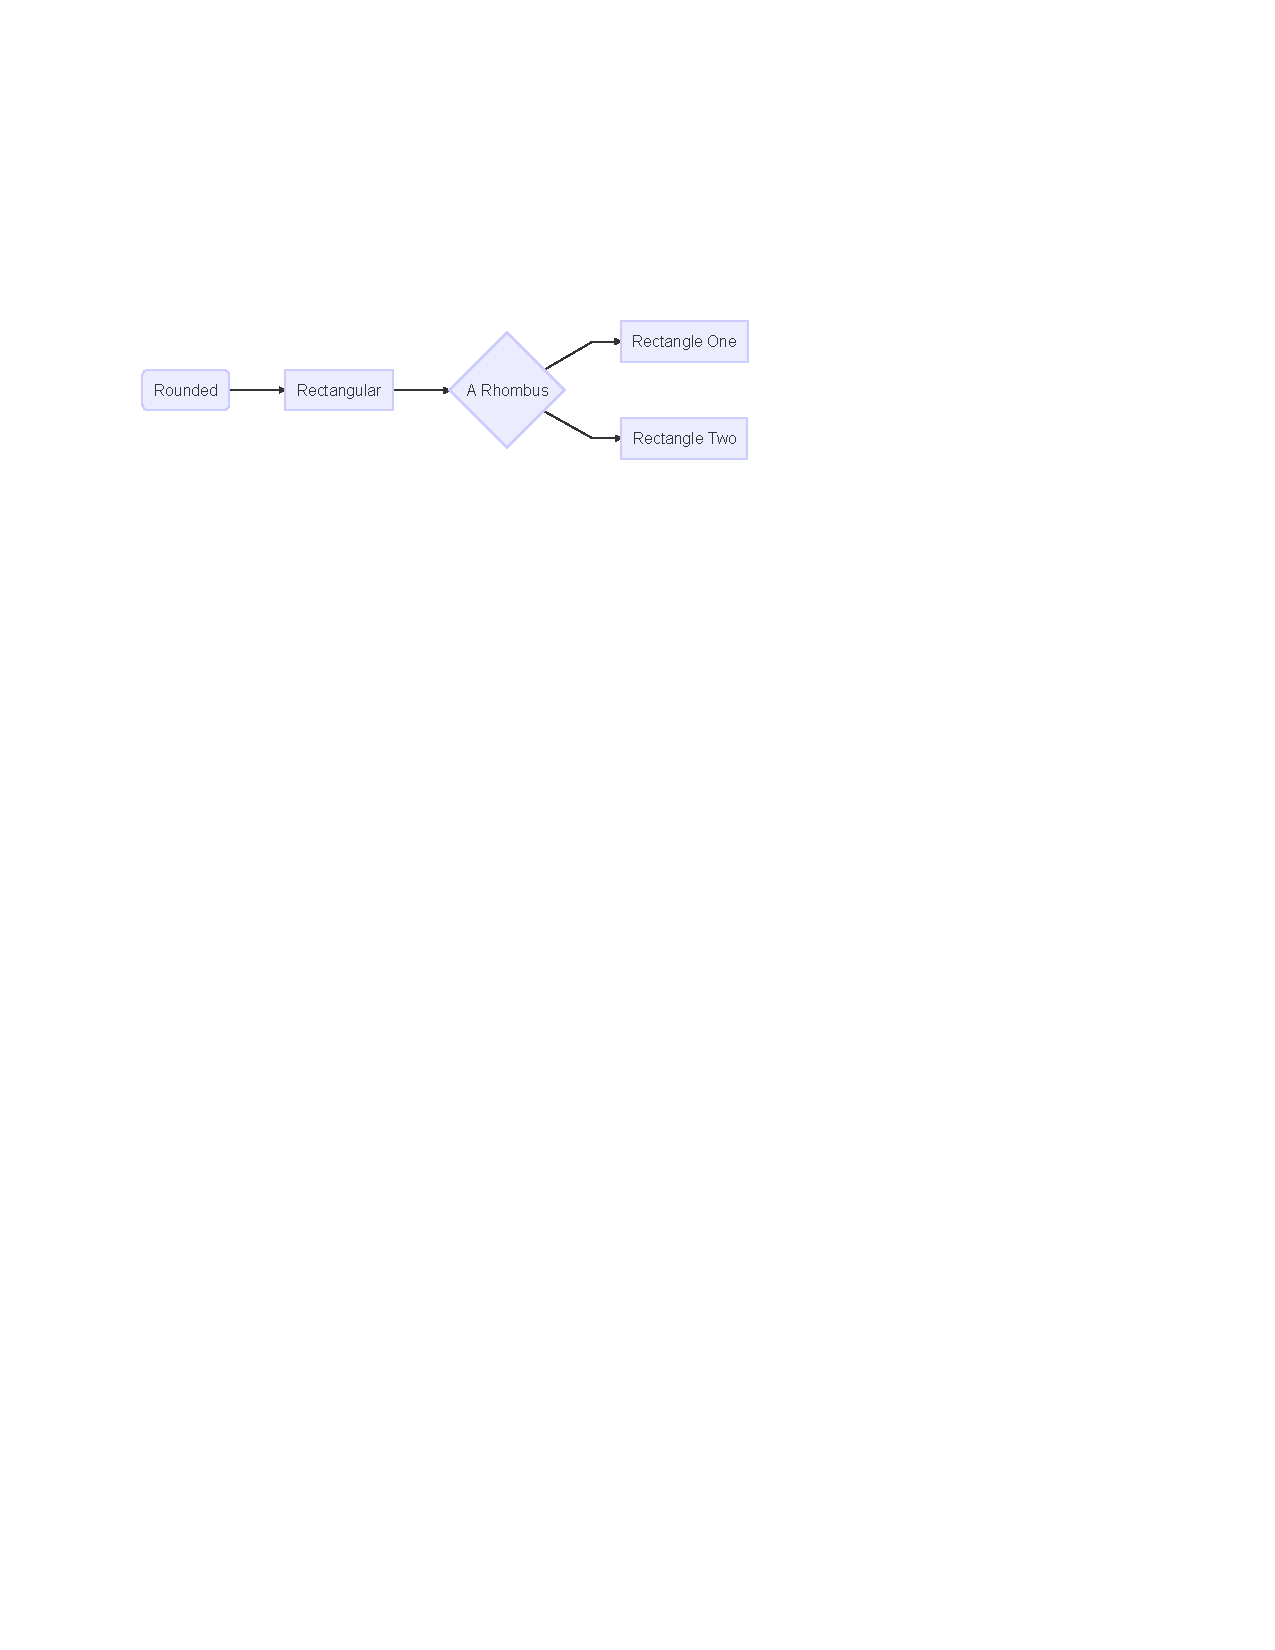
\includegraphics{./summary_files/figure-pdf/unnamed-chunk-4-6.pdf}

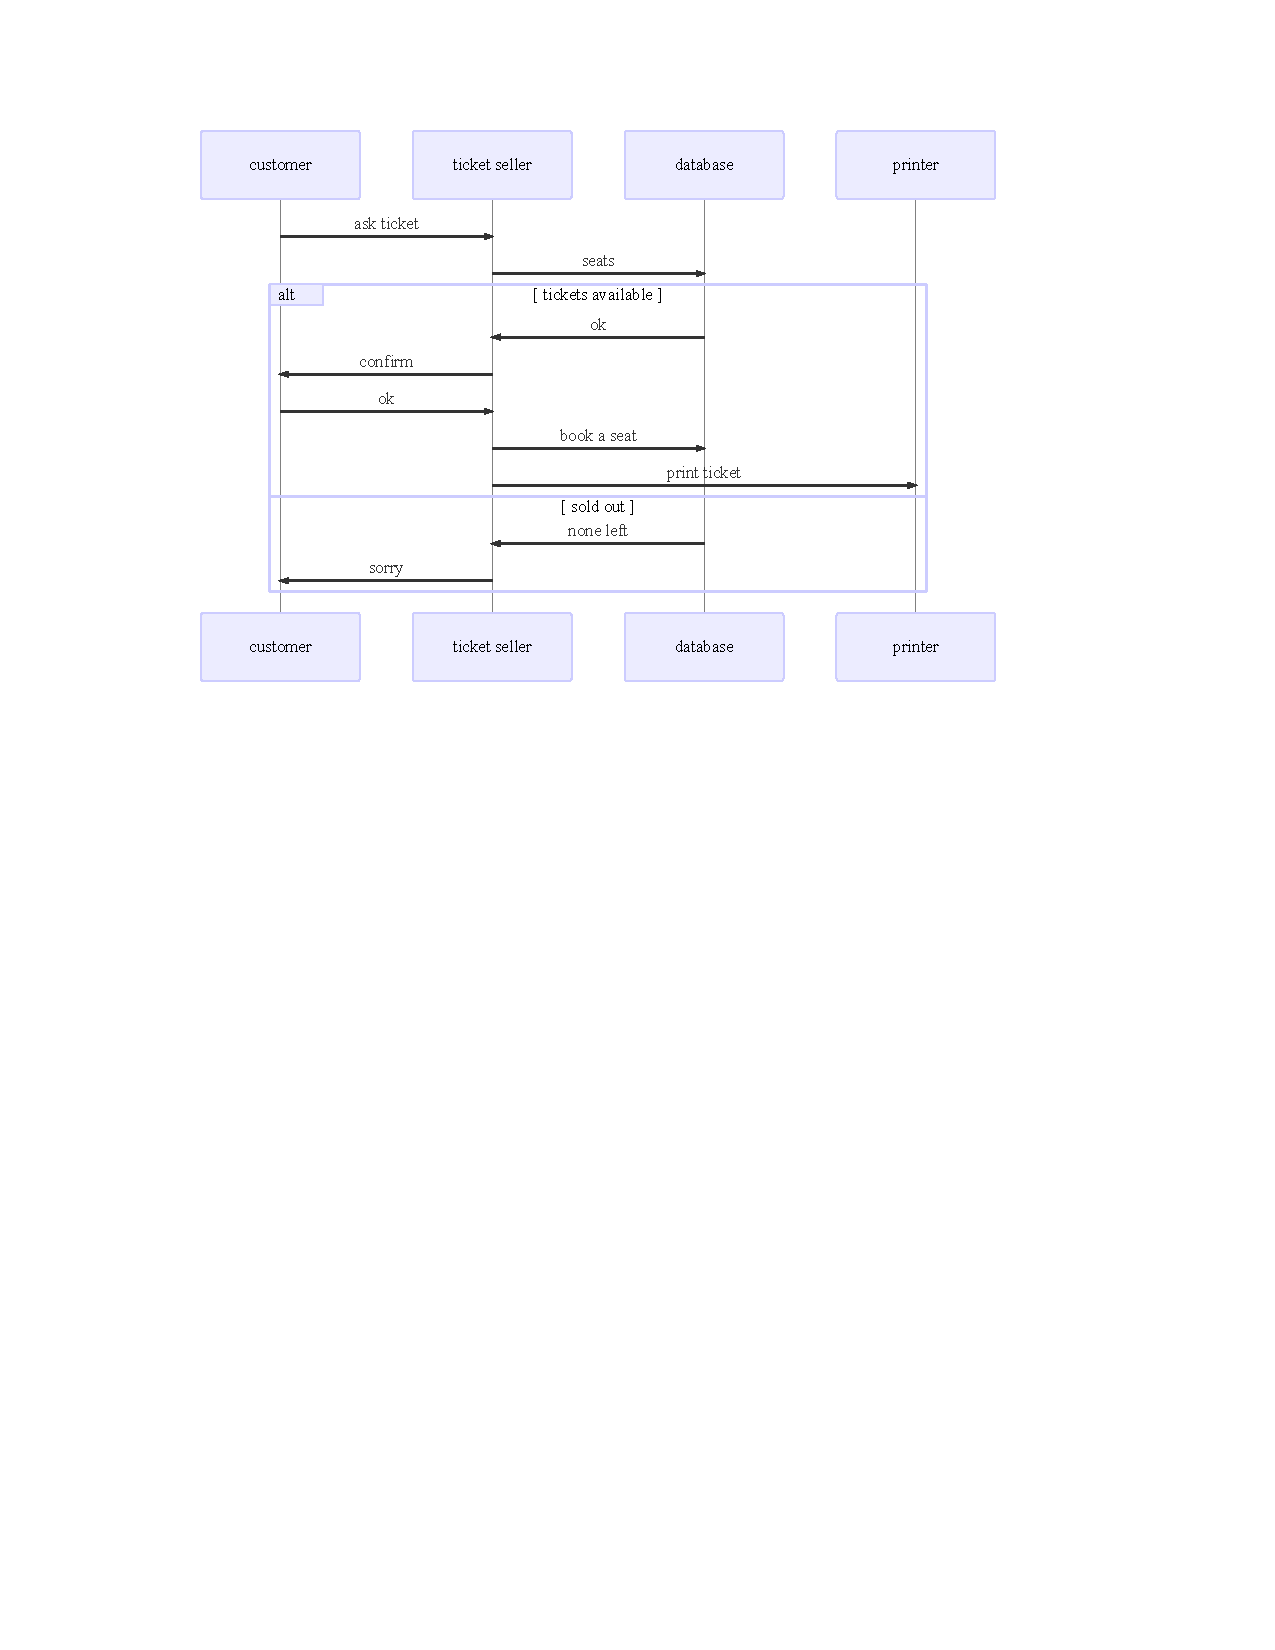
\includegraphics{./summary_files/figure-pdf/unnamed-chunk-5-1.pdf}

\bookmarksetup{startatroot}

\hypertarget{references}{%
\chapter*{References}\label{references}}
\addcontentsline{toc}{chapter}{References}

\markboth{References}{References}

\hypertarget{refs}{}
\begin{CSLReferences}{0}{0}
\end{CSLReferences}


\backmatter

\printindex

\end{document}
